% Options for packages loaded elsewhere
\PassOptionsToPackage{unicode}{hyperref}
\PassOptionsToPackage{hyphens}{url}
\PassOptionsToPackage{dvipsnames,svgnames,x11names}{xcolor}
%
\documentclass[
  letterpaper,
  DIV=11,
  numbers=noendperiod,
  oneside]{scrartcl}

\usepackage{amsmath,amssymb}
\usepackage{iftex}
\ifPDFTeX
  \usepackage[T1]{fontenc}
  \usepackage[utf8]{inputenc}
  \usepackage{textcomp} % provide euro and other symbols
\else % if luatex or xetex
  \usepackage{unicode-math}
  \defaultfontfeatures{Scale=MatchLowercase}
  \defaultfontfeatures[\rmfamily]{Ligatures=TeX,Scale=1}
\fi
\usepackage{lmodern}
\ifPDFTeX\else  
    % xetex/luatex font selection
\fi
% Use upquote if available, for straight quotes in verbatim environments
\IfFileExists{upquote.sty}{\usepackage{upquote}}{}
\IfFileExists{microtype.sty}{% use microtype if available
  \usepackage[]{microtype}
  \UseMicrotypeSet[protrusion]{basicmath} % disable protrusion for tt fonts
}{}
\makeatletter
\@ifundefined{KOMAClassName}{% if non-KOMA class
  \IfFileExists{parskip.sty}{%
    \usepackage{parskip}
  }{% else
    \setlength{\parindent}{0pt}
    \setlength{\parskip}{6pt plus 2pt minus 1pt}}
}{% if KOMA class
  \KOMAoptions{parskip=half}}
\makeatother
\usepackage{xcolor}
\usepackage[left=1in,marginparwidth=2.0666666666667in,textwidth=4.1333333333333in,marginparsep=0.3in]{geometry}
\setlength{\emergencystretch}{3em} % prevent overfull lines
\setcounter{secnumdepth}{-\maxdimen} % remove section numbering
% Make \paragraph and \subparagraph free-standing
\makeatletter
\ifx\paragraph\undefined\else
  \let\oldparagraph\paragraph
  \renewcommand{\paragraph}{
    \@ifstar
      \xxxParagraphStar
      \xxxParagraphNoStar
  }
  \newcommand{\xxxParagraphStar}[1]{\oldparagraph*{#1}\mbox{}}
  \newcommand{\xxxParagraphNoStar}[1]{\oldparagraph{#1}\mbox{}}
\fi
\ifx\subparagraph\undefined\else
  \let\oldsubparagraph\subparagraph
  \renewcommand{\subparagraph}{
    \@ifstar
      \xxxSubParagraphStar
      \xxxSubParagraphNoStar
  }
  \newcommand{\xxxSubParagraphStar}[1]{\oldsubparagraph*{#1}\mbox{}}
  \newcommand{\xxxSubParagraphNoStar}[1]{\oldsubparagraph{#1}\mbox{}}
\fi
\makeatother


\providecommand{\tightlist}{%
  \setlength{\itemsep}{0pt}\setlength{\parskip}{0pt}}\usepackage{longtable,booktabs,array}
\usepackage{calc} % for calculating minipage widths
% Correct order of tables after \paragraph or \subparagraph
\usepackage{etoolbox}
\makeatletter
\patchcmd\longtable{\par}{\if@noskipsec\mbox{}\fi\par}{}{}
\makeatother
% Allow footnotes in longtable head/foot
\IfFileExists{footnotehyper.sty}{\usepackage{footnotehyper}}{\usepackage{footnote}}
\makesavenoteenv{longtable}
\usepackage{graphicx}
\makeatletter
\newsavebox\pandoc@box
\newcommand*\pandocbounded[1]{% scales image to fit in text height/width
  \sbox\pandoc@box{#1}%
  \Gscale@div\@tempa{\textheight}{\dimexpr\ht\pandoc@box+\dp\pandoc@box\relax}%
  \Gscale@div\@tempb{\linewidth}{\wd\pandoc@box}%
  \ifdim\@tempb\p@<\@tempa\p@\let\@tempa\@tempb\fi% select the smaller of both
  \ifdim\@tempa\p@<\p@\scalebox{\@tempa}{\usebox\pandoc@box}%
  \else\usebox{\pandoc@box}%
  \fi%
}
% Set default figure placement to htbp
\def\fps@figure{htbp}
\makeatother

% load packages
\usepackage{geometry}
\usepackage{xcolor}
\usepackage{eso-pic}
\usepackage{fancyhdr}
\usepackage{sectsty}
\usepackage{fontspec}
\usepackage{titlesec}

%% Set page size with a wider right margin
\geometry{a4paper, total={170mm,257mm}, left=20mm, top=20mm, bottom=20mm, right=50mm}

%% Let's define some colours
\definecolor{light}{HTML}{E6E6FA}
\definecolor{highlight}{HTML}{800080}
\definecolor{dark}{HTML}{330033}

%% Let's add the border on the right hand side 
% \AddToShipoutPicture{% 
%     \AtPageLowerLeft{% 
%         \put(\LenToUnit{\dimexpr\paperwidth-3cm},0){% 
%             \color{light}\rule{3cm}{\LenToUnit\paperheight}%
%           }%
%      }%
%      % logo
%     \AtPageLowerLeft{% start the bar at the bottom right of the page
%         \put(\LenToUnit{\dimexpr\paperwidth-2.25cm},27.2cm){% move it to the top right
%             \color{light}
\includegraphics[width=1.5cm]{_extensions/nrennie/PrettyPDF/logo.png}
%           }%
%      }%
% }

%% Style the page number
\fancypagestyle{mystyle}{
  \fancyhf{}
  \renewcommand\headrulewidth{0pt}
  \fancyfoot[R]{\thepage}
  \fancyfootoffset{3.5cm}
}
\setlength{\footskip}{20pt}

%% style the chapter/section fonts
\chapterfont{\color{dark}\fontsize{20}{16.8}\selectfont}
\sectionfont{\color{dark}\fontsize{20}{16.8}\selectfont}
\subsectionfont{\color{dark}\fontsize{14}{16.8}\selectfont}
\titleformat{\subsection}
  {\sffamily\Large\bfseries}{\thesection}{1em}{}[{\titlerule[0.8pt]}]
  
% left align title
\makeatletter
\renewcommand{\maketitle}{\bgroup\setlength{\parindent}{0pt}
\begin{flushleft}
  {\sffamily\huge\textbf{\MakeUppercase{\@title}}} \vspace{0.3cm} \newline
  {\Large {\@subtitle}} \newline
  \@author
\end{flushleft}\egroup
}
\makeatother

%% Use some custom fonts
\setsansfont{Jost}[
    Path=_extensions/nrennie/PrettyPDF/Jost/,
    Scale=0.9,
    Extension = .ttf,
    UprightFont=*-Regular,
    BoldFont=*-Bold,
    ItalicFont=*-Italic,
    ]

\setmainfont{GentiumPlus}[
    Path=_extensions/nrennie/PrettyPDF/GentiumPlus/,
    Scale=1.0,
    Extension = .ttf,
    UprightFont=*-Regular,
    BoldFont=*-Bold,
    ItalicFont=*-Italic,
    ]
\KOMAoption{captions}{tableheading}
\makeatletter
\@ifpackageloaded{caption}{}{\usepackage{caption}}
\AtBeginDocument{%
\ifdefined\contentsname
  \renewcommand*\contentsname{Table of contents}
\else
  \newcommand\contentsname{Table of contents}
\fi
\ifdefined\listfigurename
  \renewcommand*\listfigurename{List of Figures}
\else
  \newcommand\listfigurename{List of Figures}
\fi
\ifdefined\listtablename
  \renewcommand*\listtablename{List of Tables}
\else
  \newcommand\listtablename{List of Tables}
\fi
\ifdefined\figurename
  \renewcommand*\figurename{Figure}
\else
  \newcommand\figurename{Figure}
\fi
\ifdefined\tablename
  \renewcommand*\tablename{Table}
\else
  \newcommand\tablename{Table}
\fi
}
\@ifpackageloaded{float}{}{\usepackage{float}}
\floatstyle{ruled}
\@ifundefined{c@chapter}{\newfloat{codelisting}{h}{lop}}{\newfloat{codelisting}{h}{lop}[chapter]}
\floatname{codelisting}{Listing}
\newcommand*\listoflistings{\listof{codelisting}{List of Listings}}
\makeatother
\makeatletter
\makeatother
\makeatletter
\@ifpackageloaded{caption}{}{\usepackage{caption}}
\@ifpackageloaded{subcaption}{}{\usepackage{subcaption}}
\makeatother
\makeatletter
\@ifpackageloaded{tcolorbox}{}{\usepackage[skins,breakable]{tcolorbox}}
\makeatother
\makeatletter
\@ifundefined{shadecolor}{\definecolor{shadecolor}{rgb}{.97, .97, .97}}{}
\makeatother
\makeatletter
\@ifundefined{codebgcolor}{\definecolor{codebgcolor}{named}{light}}{}
\makeatother
\makeatletter
\ifdefined\Shaded\renewenvironment{Shaded}{\begin{tcolorbox}[sharp corners, enhanced, boxrule=0pt, breakable, frame hidden, colback={codebgcolor}]}{\end{tcolorbox}}\fi
\makeatother
\makeatletter
\@ifpackageloaded{sidenotes}{}{\usepackage{sidenotes}}
\@ifpackageloaded{marginnote}{}{\usepackage{marginnote}}
\makeatother

\usepackage{bookmark}

\IfFileExists{xurl.sty}{\usepackage{xurl}}{} % add URL line breaks if available
\urlstyle{same} % disable monospaced font for URLs
\hypersetup{
  pdftitle={Endless Summer},
  pdfauthor={Martin Roberts},
  colorlinks=true,
  linkcolor={highlight},
  filecolor={Maroon},
  citecolor={Blue},
  urlcolor={highlight},
  pdfcreator={LaTeX via pandoc}}


\title{Endless Summer}
\usepackage{etoolbox}
\makeatletter
\providecommand{\subtitle}[1]{% add subtitle to \maketitle
  \apptocmd{\@title}{\par {\large #1 \par}}{}{}
}
\makeatother
\subtitle{Transcultural Geographies of city pop Art}
\author{Martin Roberts}
\date{2025-03-18}

\begin{document}
\maketitle

\pagestyle{mystyle}


\textbf{And Suddenly There Was city pop: The Global Dimensions of the
Retrograde Formation of a Japanese Popular Music Genre}\\
University of Amsterdam, 19-21 March 2025

\href{abstract.qmd}{Abstract}

\begin{center}\rule{0.5\linewidth}{0.5pt}\end{center}

\begin{quote}
So many of city pop's greatest songs are about the hottest season and
it's a perfect match to the vibe of the genre. \ldots{} Anything Summer
related is a safe bet for a city pop aesthetic.

Van Paugam,
``\href{https://vanpaugam.com/blog/2020/10/20/city-pop-aesthetics}{\textbf{city
pop Aesthetics}}'' (October 2021)
\end{quote}

\subsubsection{I. California Dreaming}\label{i.-california-dreaming}

My original intention when I first proposed this paper was to focus not
on the music of city pop itself but on the artwork of Hiroshi Nagai that
has become its visual counterpart. That was before I actually did my
homework and discovered that the work has already been substantially
done for me---most notably by our dear colleague Toshiyuki Ohwada, whose
excellent article ``city pop's America'' is among the three essays
included in the catalog to the exhibition that ran at the Japan
Foundation Gallery in Sydney, Australia, from September 2020 to January
2021, titled
\href{https://sydney.jpf.go.jp/events/hiroshi-nagai-paintings-for-music/?fbclid=IwY2xjawI-ln5leHRuA2FlbQIxMAABHeUKRUj04Mc1iZN3DLiHTb9vlyObwcnLlw9RSAhx0Qs9AoYexaWgypC6bA_aem_H1QOj7XPApKfEvNOOAXjdA}{\textbf{Hiroshi
Nagai: Paintings for Music}}, concurrently with a second exhibition,
\href{https://sydney.jpf.go.jp/events/city-pop-inspired-nostalgia/}{\textbf{city
pop: Inspired Nostalgia}}. Since the 68-page
\href{https://sydney.jpf.go.jp/jpf/jpfmedia/JPF-HNCatalogue-R7-Issuu.pdf}{\textbf{exhibition
catalog}} to the Nagai exhibition is available online, I can only refer
colleagues to it for the background material that I had originally
planned to provide. Indeed, since the YouTube algorithm launched the
viral success of Mariya Takeuchi's 1984 hit ``Plastic Love''
(\href{https://www.japantimes.co.jp/culture/2018/11/17/music/mariya-takeuchi-pop-genius-behind-2018s-surprise-online-smash-hit-japan/}{St.~Michel,
2018}, and the subsequent release by Light in the Attic Records of the
first in its
\href{https://lightintheattic.net/collections/v-a-pacific-breeze/products/pacific-breeze-japanese-city-pop-aor-boogie-1976-1986}{\textbf{Pacific
Breeze}} compilation series (2019), Nagai's work has become an
increasing focus of attention as the visual representative of city pop.
As with Korea's rapid---not to mention lucrative--- international
institutionalization of K-pop, the Japan Foundation has been quick to
seize an opportunity to flex some Japanese soft power of its own. In
Spring 2023 the Bunkamura gallery in Shibuya hosted a homegrown
retrospective,
\href{https://www.bunkamura.co.jp/gallery/exhibition/230301nagai.html}{\textbf{永井博
The Journey Never Ends}}. In addition to this institutional presence,
Nagai's images are today ubiquitous on YouTube's infinity pool of city
pop playlists and fan videos, as well as on countless Instagram
accounts, Pinterest mood boards, desktop wallpapers, and animated gifs.

Given all this, I will not be reprising here Nagai's work and his
involvement in both the origins and afterlife of city pop, from the 1979
publication of his book \textbf{A Long Vacation} and its featuring on
Eiichi Ohtaki's city pop classic of the same name (1981) to the Light in
the Attic compilations and beyond. Nor will I be framing Nagai's
Californian dreamscapes in relation to the thematics of pastiche and
exoticism elaborated in Shuhei Hosokawa's wonderful concept of ``soy
sauce music'' and Haruomi Hosono's Tropical Dandy alter ego. The
abundance of existing documentation at least clears some space for us to
begin exploring some less visited islands in the archipelago. What I
want to do here is to pick up where the existing discussion leaves off
and consider some of its more interesting threads---for example, the
observation by Yamato Shiine (editor of \textbf{Popeye} magazine), cited
by Toshiyuki Ohwada, about how the lifestyle sports of surfing, skate
boarding, and hang gliding popularized in 1970s California were about
weightlessness, a sense of floating, and a feeling of equilibrium
(Shiine 2010, cited in Ohwada 2020), prompting the following point from
Ohwada:

\begin{quote}
This abstract sense of floating can be seen in Hiroshi Nagai's work. Its
sense of weightlessness is probably derived from the artist's origins in
surrealism in addition to a shared sensibility of American west coast
sports (Ohwada 2020: 11).
\end{quote}

What interests me here (in addition to the impact of Surrealism on
Nagai's work) is that this is a point about aesthetics, since aesthetics
is what I want to focus on in what follows, albeit in a different sense
from how that term has been tradition understood in art history.

While the bulk of existing scholarship on city pop to date has been
historical, in terms of contextualizing the emergence of the style
itself in relation to larger economic forces---basically the bubble
economy of the 1980s, while it lasted---and their socio-cultural shifts,
as well as the more recent history of ``city pop'' itself as a
retroactive form of nostalgia for a future that never materialized
(Sommer, DATE), my orientation here is more resolutely presentist. I am
interested in the here and now of city pop as a dynamic force of
contemporary cultural content. I am interested not only in the economic
and socio-cultural forces that generated it, but the new media and
cultural practices being generated from it---in the literal sense, as we
will see. Mainly, though, I am interested in city pop as a contemporary
example of what has come to be known as an Internet aesthetic.

\subsubsection{II. Summer Feeling}\label{ii.-summer-feeling}

To elaborate on this, some methodological observations are first
necessary. From a disciplinary standpoint, city pop has been primarily
approached to date \textbf{as music}---that is, within the discursive
formation of popular music studies, specifically the history of Japanese
popular music, and global/transnational music production, reception, and
consumption. Within this formation, while Hiroshi Nagai's illustrations
are acknowledged to be a key visual component of city pop aesthetics,
they are still conceived as somewhat auxiliary to it; primarily, it is
taken for granted, ``city pop'' refers to a style of \textbf{music},
albeit one with a strong visual counterpart, but primarily music
nonetheless. Much the same could be said of the visual components of
other Japanese popular music genres, notably Shibuya-kei and, of course,
Visual-kei. But it's precisely this music-centric conception of city pop
that I want to challenge here, and not just to suggest that Hiroshi
Nagai's artwork is as central to city pop as the musical artists who
produced it. One of the key limitations of the popular-music-studies
approach, which has already begun to emerge in its difficulty in coming
to grips with new aesthetic forms such as vaporwave or lo-fi hip hop, is
its inadequacy in conceptualizing the catalytic role of social media in
their production and circulation. While they are obviously referenced as
having ``originated'' on social platforms and/or ``the internet'', it's
still assumed that what the primary object of attention are and should
be specifically musical practices and aesthetics. While city pop is
frequently mentioned in connection with Internet aesthetics like
vaporwave or future funk (``Introduction'': 4), such references are
typically made only in passing before returning to the music itself, its
artists, and their history. YouTube, while important, is no more than a
platform for the music rather than an active agent of cultural
production. Against this framework, I argue that global cultural forms
such as city pop, Lo-Fi Hip Hop, or the fifty shades of vaporwave should
be approached not as primarily musical styles alone but as
\textbf{aesthetics}, in which music is only one element with equivalent
status to artwork, video, fashion, memes, and other forms of digital
content.

So what exactly \textbf{is} an ``aesthetic'' in this context, and what
does it mean to reframe city pop as an aesthetic, rather than what it
rather obviously appears to be: a historical genre of Japanese popular
music? In what is to my knowledge the only academic source to date to
have explored the concept of the aesthetic in theoretical terms,
\href{https://firstmonday.org/ojs/index.php/fm/article/view/12723}{Guilherme
Giolo and Michaël Berghman} (2023) suggest that traditional conceptual
frameworks such as genre, lifestyle, or subculture are no longer
adequate to understanding the contemporary modalities of cultural
identity and creativity. Instead, they explore the ubiquitous popular
concept of the ``aesthetic'' as the key component of a new analytical
framework. What does an ``aesthetic'' in this contemporary sense consist
of? We might start by examining the entry on
\href{https://aesthetics.fandom.com/wiki/City_Pop}{``city pop''} on the
\href{https://aesthetics.fandom.com/wiki/Aesthetics_Wiki}{Aesthetics
Wiki}, a vast online catalogue of aesthetic styles from ``Algorave'' to
``Zombie Apocalyse'', ``Dark Academia'' to ``Visual-kei'',
``Cottagecore'' to ``Witch House''. Like many of the other entries about
aesthetics that the reader is already acquainted with, however, the city
pop entry, while a useful introduction, brings few surprises, opening
with a bland definition of it as ``a subgenre of Pop music from Japan''.
The remainder of the entry is a walkthrough of everything that everyone
at this conference already knows, with the obligatory references to
1970s American AOR, YMO, and the California Dreaming of Hiroshi Nagai.
What the entry doesn't get us much closer to, however, is understanding
why city pop can be considered not just as a J-pop subgenre but an
\textbf{aesthetic}, and for this we need to go back to Giolo and
Berghman.

One of the defining components of what Giolo and Berghman call Internet
aesthetics is their association with certain kinds of experience, and
the corresponding feelings evoked by the memory of that experience: the
experience of living in the world of 1950s America, for example, or the
world of Harry Potter; the experience of living in a dystopian future;
or, one might add, the experience of living on the American West Coast
in the 1970s, or in Tokyo at the height of the bubble economy. While
music is a key component of such experiences, it is only one modality
within a larger cultural world. Imaginatively speaking, aesthetics
recall the fantasy worlds of videogames and LARPing:

\begin{quote}
Experiences (and, likely, their importance for Internet aesthetics) seem
to be even more evident in the titles of playlists associated with
different aesthetics: ``You are studying in a haunted library with
ghosts'' (dark academia playlist), ``You found the entrance to a secret
garden'', ``You are falling for the protagonist in a fantasy novel''
(light royaltycore), or ``A playlist for old money living in the French
countryside'' (light academia). Even clearer here, multiple objects
(songs) are grouped and given symbolic meaning under a new interpretive
key. This key is experience-centered. Thus, it seems acceptable to
assume that experience is also the goal of an Internet aesthetic: to
become someone different, \emph{to feel as if living in a different
time} (2023) {[}Emphasis mine{]}
\end{quote}

The dominant musical modality of aesthetics is the \textbf{playlist},
and playlists can be thought of as scripts or catalysts for certain
kinds of experience: the dark cinematic vibe of \emph{film noir} in
jazz; chillout-room electronica; the moody self-absorption of shoegaze;
the entire ``After Hours'' DJ session collection. Although originating
in the album-based formats of the 1970s and 1980s, city pop today is
something that we \textbf{experience} as much as just listen to,
something that conjures up a particular \textbf{structure of feeling}
(as Raymond Williams used to call it); and the primary way we experience
it is through the playlist, whether in the form of the compilation
release (\textbf{Pacific Breeze}) or the endless-summer playlists of
YouTube and Spotify. With the advent of the playlist, all music became
background music---music \textbf{for} something, that creates the
ambience for certain kinds of experience: studying, barbecueing, driving
at night, lovemaking, being depressed after a breakup. Music has long
had this function, of course; its origins go back to the so-called
``mood music'' of the 1950s, when stereophonic recording began to turn
it into an environment: \textbf{Music For Lovers}; \textbf{Soothing
Sounds for Baby}; and several decades later, \textbf{Music For
Airports}. Since the 1990s, mood music has been replaced by the concept
of \textbf{vibe}, but both are arguably about music as a catalyst for
shared experience (or the imagination of such experience) and the
structures of feeling associated with them. It's no coincidence that the
current generation of city pop fans around the globe are too young to
have lived through the decades to which it provided the musical
soundtrack, since \textbf{anemoia}---defined as nostalgia for something
one never experienced directly---is one of the key constituents of
Internet aesthetics. To listen to an album today such as Tatsuro
Yamashita's appropriately-titled \textbf{For You} (1982), most of us can
only dream of another, better time and place, when Japan was still
surfing the economic wave and the prevailing mood was for glamour and
partying. A decade later, after the bubble had burst, while Yasuharu
Konishi's Readymade Records continued to party like it was (not yet)
1999, the vibe of Shibuya-kei led by Crue-el and Trattoria Records was
more edgy, more indie, more circumspect---Music For The Morning After.

Giolo and Berghman also emphasize the affective dimension of Internet
aesthetics, and their interviewees frequently reference feelings when
describing them:

\begin{quote}
``The aesthetics that I like really depend on my mood of the day. On
Sundays, when it's sunny, I really enjoy aesthetic images that
\emph{give me this summer feeling}'' Jane (Dutch, prefers
``cottagecore'').

Jane, who strongly connects ``cottagecore'' to morning walks, went on to
explain that in those moments the scenarios and imaginaries of this
Internet aesthetic ``flow'' into her activity, representing ``the things
I would like at that moment. \emph{They give me a warming feeling}''
(2023). {[}Emphasis mine{]}
\end{quote}

By now we are (hopefully) getting closer to understanding what it means
to describe city pop as an aeesthetic rather than just a musical genre.
Like vaporwave, like future funk, like mallsoft, like lo-fi hip hop,
city pop conjures up a particular kind of cultural-historical aesthetic
experience and a corresponding affective structure, via playlists,
imagery, and other elements. As has been much discussed in the case of
vaporwave, the dominant temperamental register is nostalgic and
melancholic, invoking a bygone era of economic optimism and
technological utopianism rendered only more poignant by the harsh
realities of the dystopian present.

\subsubsection{III. Afterlife}\label{iii.-afterlife}

If the preceding discussion has led you to consider reframing city pop
as an aesthetic, let me conclude with an example of how that aesthetic
is continuing to mutate into new forms of creative expression. One of
the characteristics of an aesthetic is that it is defined by--and can be
encoded as--a set of audiovisual stylistic parameters that constitute
its aesthetic fingerprint. As many recent studies show, the algorithms
of streaming platforms such as Spotify are based on the systematic
encoding of such styles, often referred to as a kind of musical DNA.
Spotify, for example, has three official city pop playlists,
respectively for the 1970s, 1980s, and 1990s. This algorithmic
systematization of popular music has had a number of unexpected
consequences, one of which has been the much-discussed (and
much-maligned) atomization of music genres: the explosive proliferation
of algorithmically-defined styles based solely on audience listening
data. As the website \href{https://everynoise.com/engenremap.html}{Every
Noise At Once} attests, this musical ecosystem is continuing to expand
and mutate into what The Orb might have been anticipating in their album
\emph{A Huge Ever Growing Pulsating Brain That Rules From The Centre Of
The Ultraworld}.

The other, even more frequently denounced consequence of the
parameterization of musical styles has been automation, in other words:
the algorithmic generation of styles using models trained on the styles
themselves, based on a textual prompt input by the user. While far from
alone in this respect, the music of city pop is among the styles in
question. A simple search on YouTube using terms like ``city pop ai''
quickly produces not just
\href{https://youtu.be/EaK5AQ_fnS0?si=M-9LSJysAZjHBAbu}{algorithmically-generated
playlists} but playlists of algorithmically-generated city pop music. As
Claude.ai calmy explained to me but presumably everyone here already
knows,

\begin{quote}
There is indeed a growing amount of AI-generated city pop music on
YouTube. City pop's nostalgic 80s Japanese aesthetic, with its
distinctive synthesizer sounds, funk/disco influences, and cityscapes
has made it a popular genre for AI music generation.

Many creators are using AI tools like Suno, Udio, and other music
generation platforms to create city pop tracks that emulate the style of
artists like Mariya Takeuchi, Tatsuro Yamashita, and other city pop
icons. These AI-generated tracks often feature the genre's signature
elements - jazzy chord progressions, funky bass lines, and smooth
saxophone solos.

The popularity of city pop's aesthetic combined with the increasing
capabilities of AI music generation has led to numerous channels
dedicated to sharing these AI-created city pop tracks, often paired with
anime-style visuals or cityscapes.
\end{quote}

Ending on a more reassuring note, it added that

\begin{quote}
while there's definitely AI-generated city pop on YouTube, it still
represents just a portion of the city pop content there, with many
channels still focused on sharing original city pop tracks from the
70s-80s Japanese music scene or human-created new music in that style.
\end{quote}

There are of course many ways to do this, depending on your level of
Python coding skills. On Udio, the following prompt generated a musical
wallpaper sample---inevitably titled ``Neon Dreams''---that was as
crushingly generic as you would expect.

\begin{quote}
Japanese city pop, 1970s era, funky beat, complex electric piano jazz
chords, synthesizer flourishes, evoking nostalgia for American
album-oriented rock and California lifestyles.
\end{quote}

While for devotees of city pop a public admission of such necromancy is
the cultural equivalent of dancing with the devil, it remains undeniable
that the style has been sucked into the jet engine along with all the
others, whose implications for the cultural environment at this point
remain unclear. Today's diffusion models are by no means limited to
musical outputs, moreover, and along with generative playlists and
music, city pop's visual components have also begun to be automated. One
of the cornerstones of today's generative media aesthetics is
\textbf{restylization}, the application of historical styles of art,
music, cinema, or other media to any kind of audiovisual content. On
generative media websites, for example, a still from a Studio Ghibli
film can be algorithmically mapped onto the movements of a dancer in a
live action video, so it appears to be an animated character that is
dancing; but the source image could equally be a medieval painting. Such
models proliferate and circulate widely on generative websites such as
\href{https://civitai.com}{CivitAI}, enabling users to customize
audiovisual content in a way similar to popular sites like
\href{https://www.midjourney.com/}{Midjourney} or
\href{https://runwayml.com/}{Runway}. On Civit AI, one can easily find
includes numerous city pop style models trained on datasets of images by
Hiroshi Nagai. These images were generated using one such model; they
are not copies of specific works, but none of them are the work of Nagai
himself.

\marginnote{\begin{footnotesize}

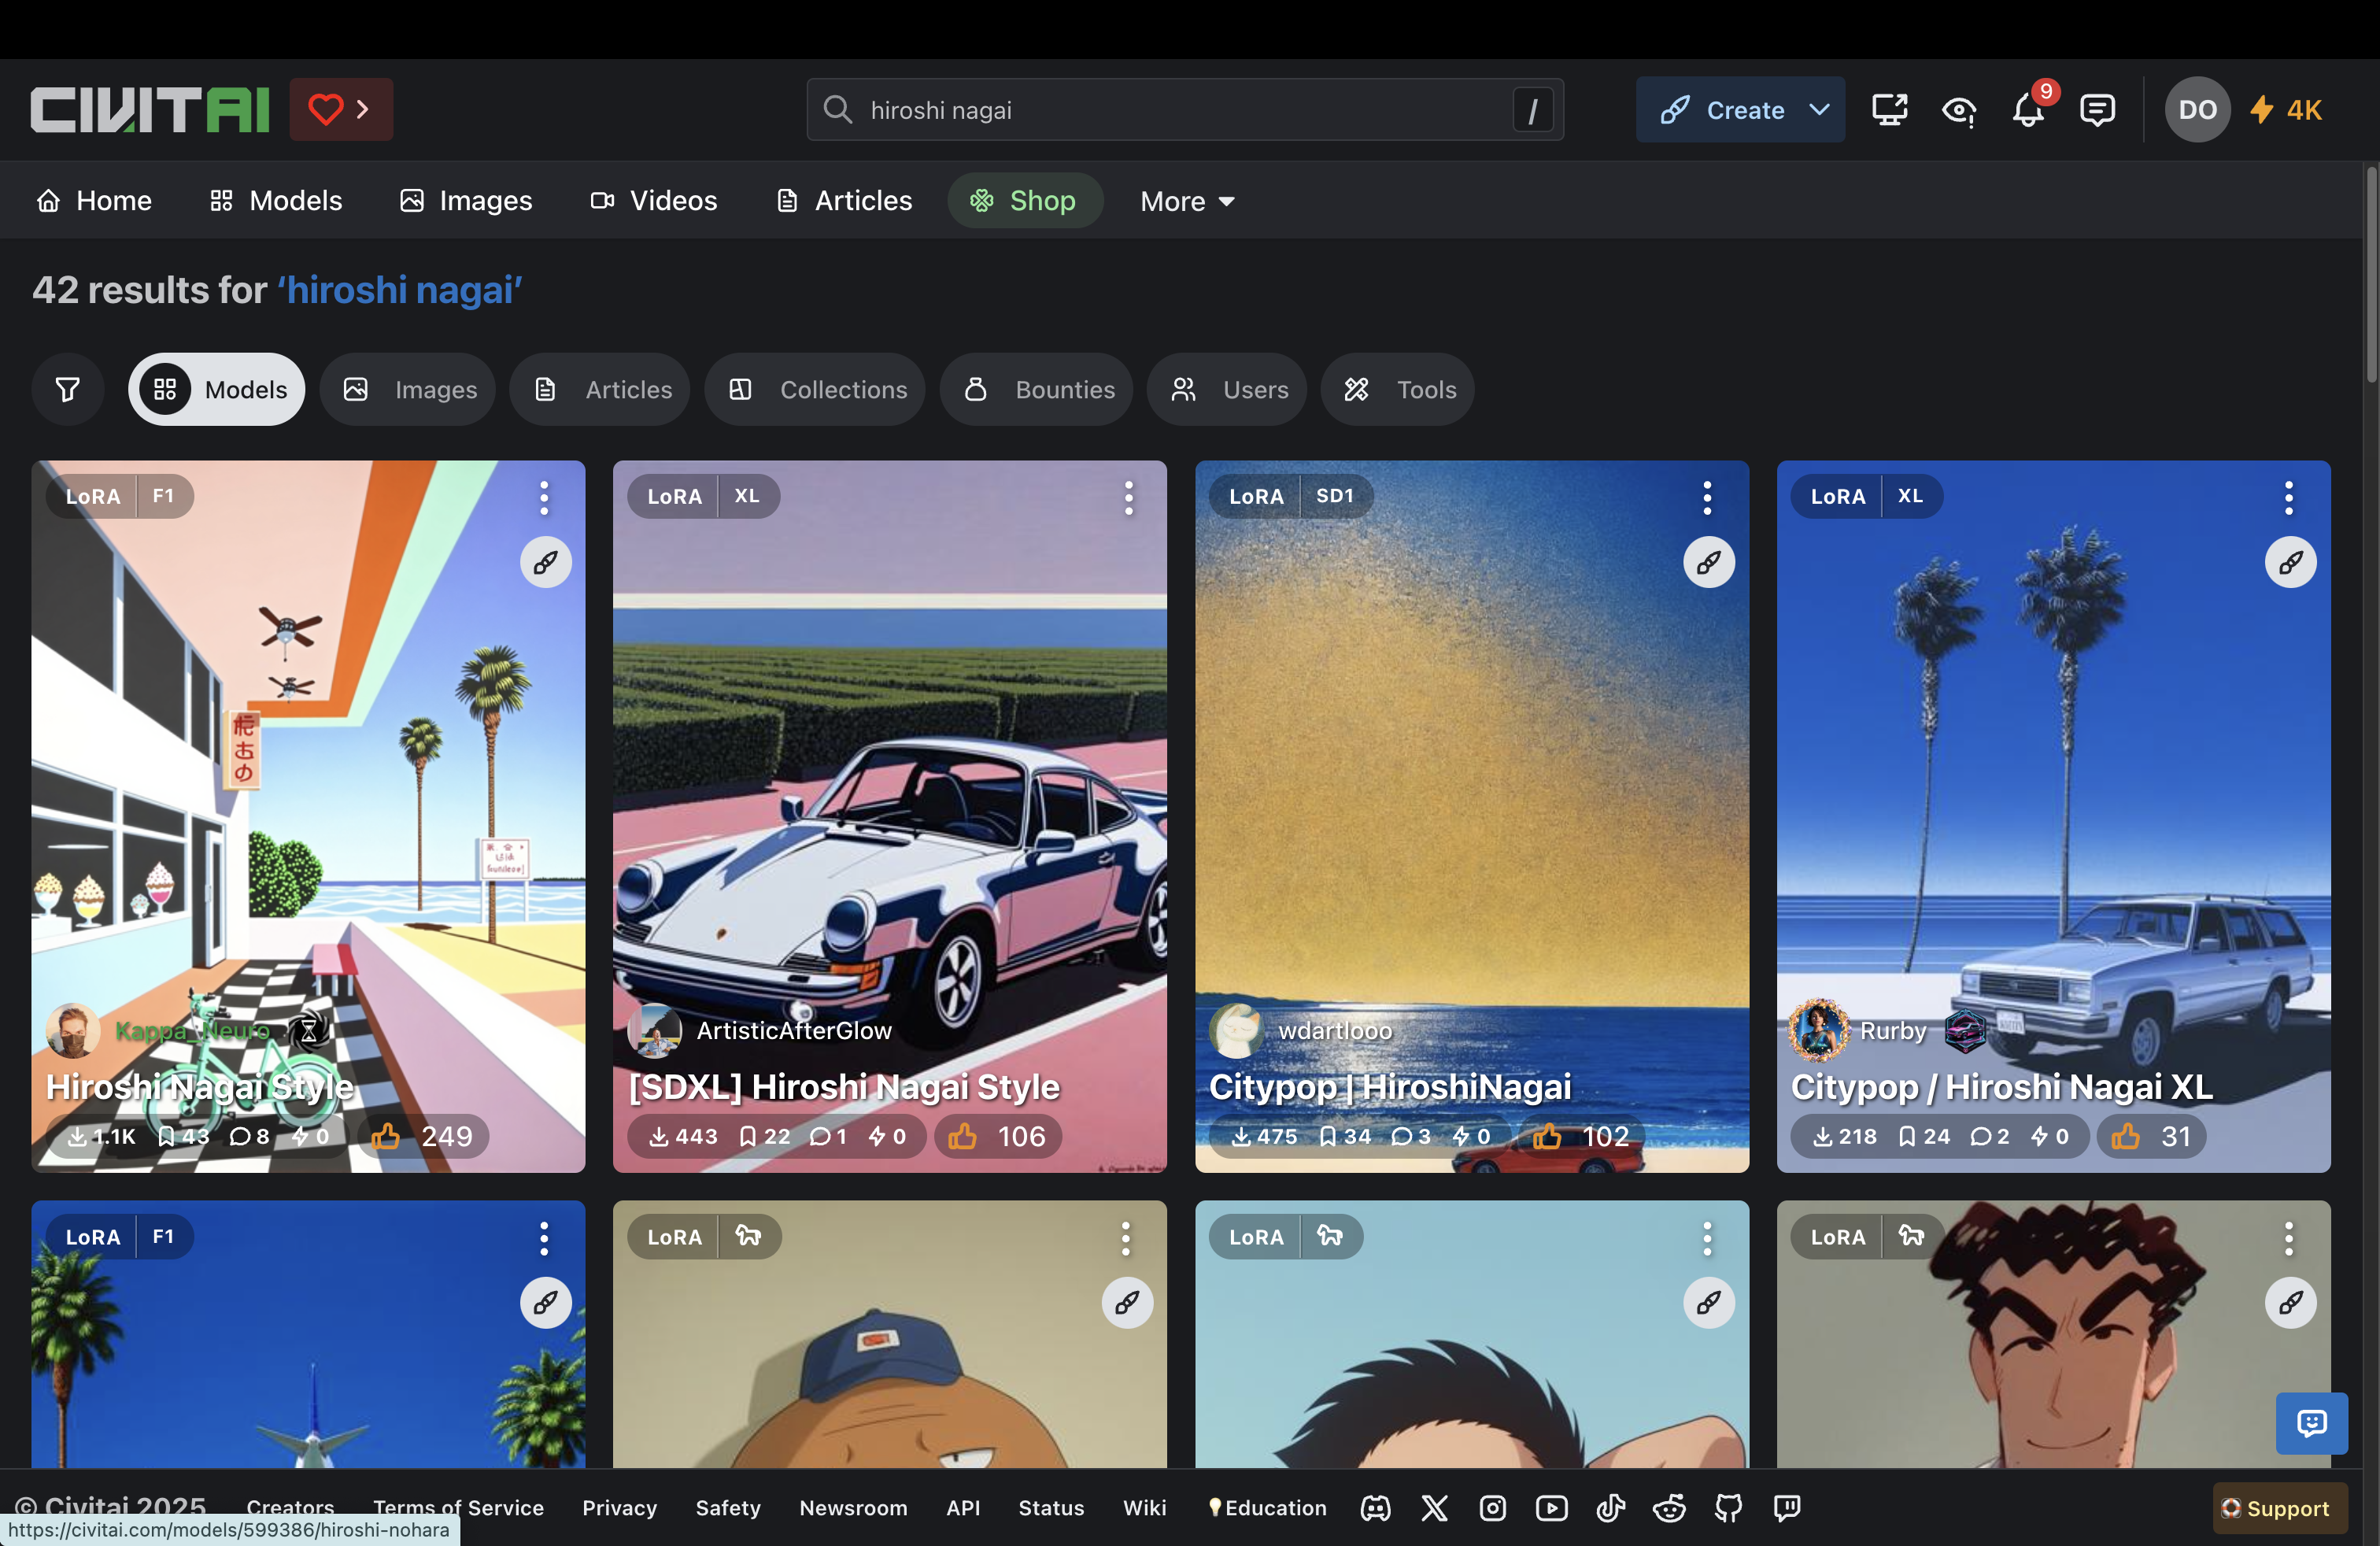
\includegraphics[width=1.04167in,height=\textheight,keepaspectratio]{img/civitai-screenshot1.png}
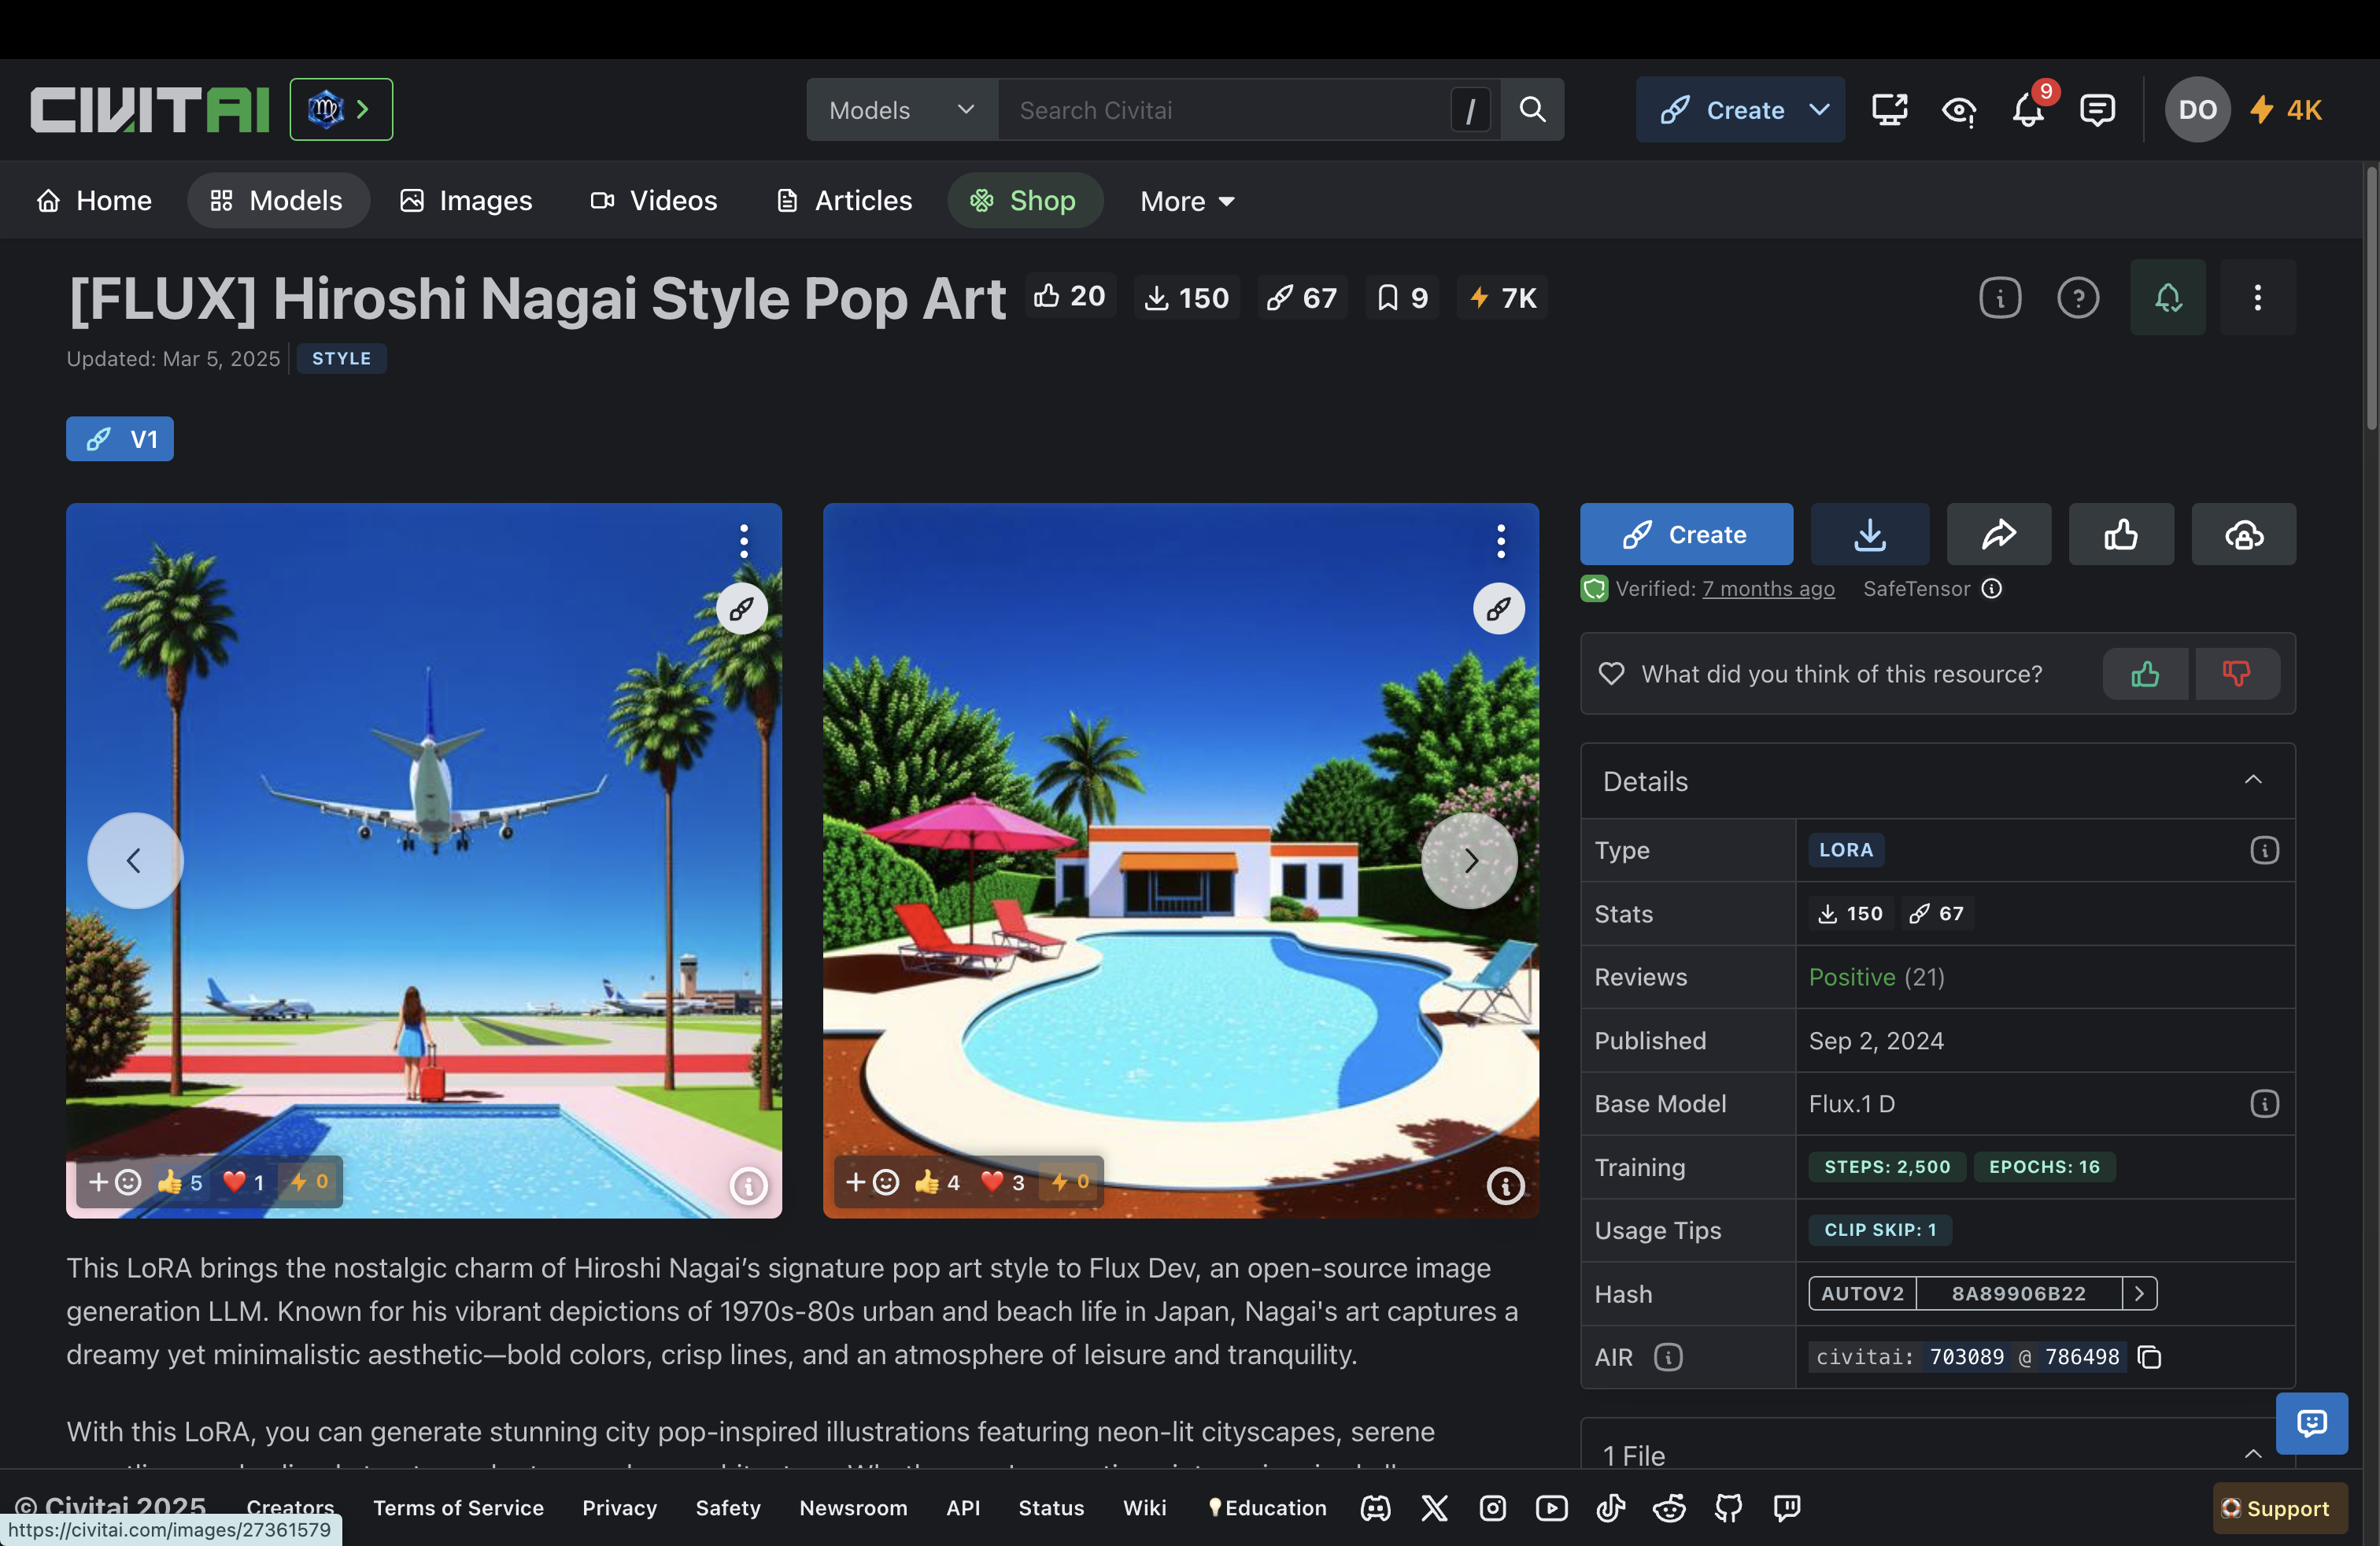
\includegraphics[width=1.04167in,height=\textheight,keepaspectratio]{img/civitai-screenshot2.png}

\end{footnotesize}}

As the text on the model page explains:

\marginnote{\begin{footnotesize}

\includegraphics[width=0.52083in,height=\textheight,keepaspectratio]{img/civitai-hiroshi-nagai1.jpeg}
\includegraphics[width=0.52083in,height=\textheight,keepaspectratio]{img/civitai-hiroshi-nagai2.jpeg}
\includegraphics[width=0.52083in,height=\textheight,keepaspectratio]{img/civitai-hiroshi-nagai3.jpeg}
\includegraphics[width=0.52083in,height=\textheight,keepaspectratio]{img/civitai-hiroshi-nagai4.jpeg}
\includegraphics[width=0.52083in,height=\textheight,keepaspectratio]{img/civitai-hiroshi-nagai5.jpeg}
\includegraphics[width=0.52083in,height=\textheight,keepaspectratio]{img/civitai-hiroshi-nagai6.jpeg}
\includegraphics[width=0.52083in,height=\textheight,keepaspectratio]{img/civitai-hiroshi-nagai7.jpeg}

\end{footnotesize}}

\begin{quote}
This LoRA brings the nostalgic charm of Hiroshi Nagai's signature pop
art style to Flux Dev, an open-source image generation LLM. Known for
his vibrant depictions of 1970s-80s urban and beach life in Japan,
Nagai's art captures a dreamy yet minimalistic aesthetic---bold colors,
crisp lines, and an atmosphere of leisure and tranquility.

With this LoRA, you can generate stunning city pop-inspired
illustrations featuring neon-lit cityscapes, serene coastlines,
palm-lined streets, and retro-modern architecture. Whether you're
creating vintage-inspired album covers, dreamy summer scenes, or classic
city pop aesthetics, this model helps you bring that unmistakable Nagai
vibe to your artwork.

This LoRA was developed just one month after the initial release of Flux
Dev, contributing early to its expanding creative possibilities. And
still, in 2025, Flux Dev remains the leading open-source image
generation LLM. Try it out and share your creations! 🚀

Created for Flux Dev by Burç Buluklu.
\end{quote}

Since images can also be used as source inputs for time-based generative
content, and animation is one of the fasting-growing areas of generative
AI, it seems likely that we may soon see generative city pop music
videos or animated short movies that that bring Hiroshi Nagai's images
to life just as the film \textbf{Loving Vincent} did with Van Gogh's
iconic paintings. I am neither condoning nor condemning these practices;
in engaging with them, I seek only to better understand them by direct
experience of their mechanisms.

city pop generative music and images raise contentious but as yet
unanswered questions about the ethics, legality, and aesthetics of media
practices in the algorithmic age: about copyright and the concept of
digital rights itself; about the place of the human in artistic
creativity; about authorship, and about the status of generative art.
Regardless of our position on such questions, new creative practices
continue to emerge and will continue to do so. The summer of city pop
may indeed turn out to be endless, but not in the way anyone back in the
heady days of the bubble economy could ever have imagined. As we look
back on city pop and its legacy, we would do well also to examine its
present, as well as its future afterlives.

\includegraphics[width=3.125in,height=\textheight,keepaspectratio]{img/hiroshi-nagai-airport.png}

\begin{center}\rule{0.5\linewidth}{0.5pt}\end{center}

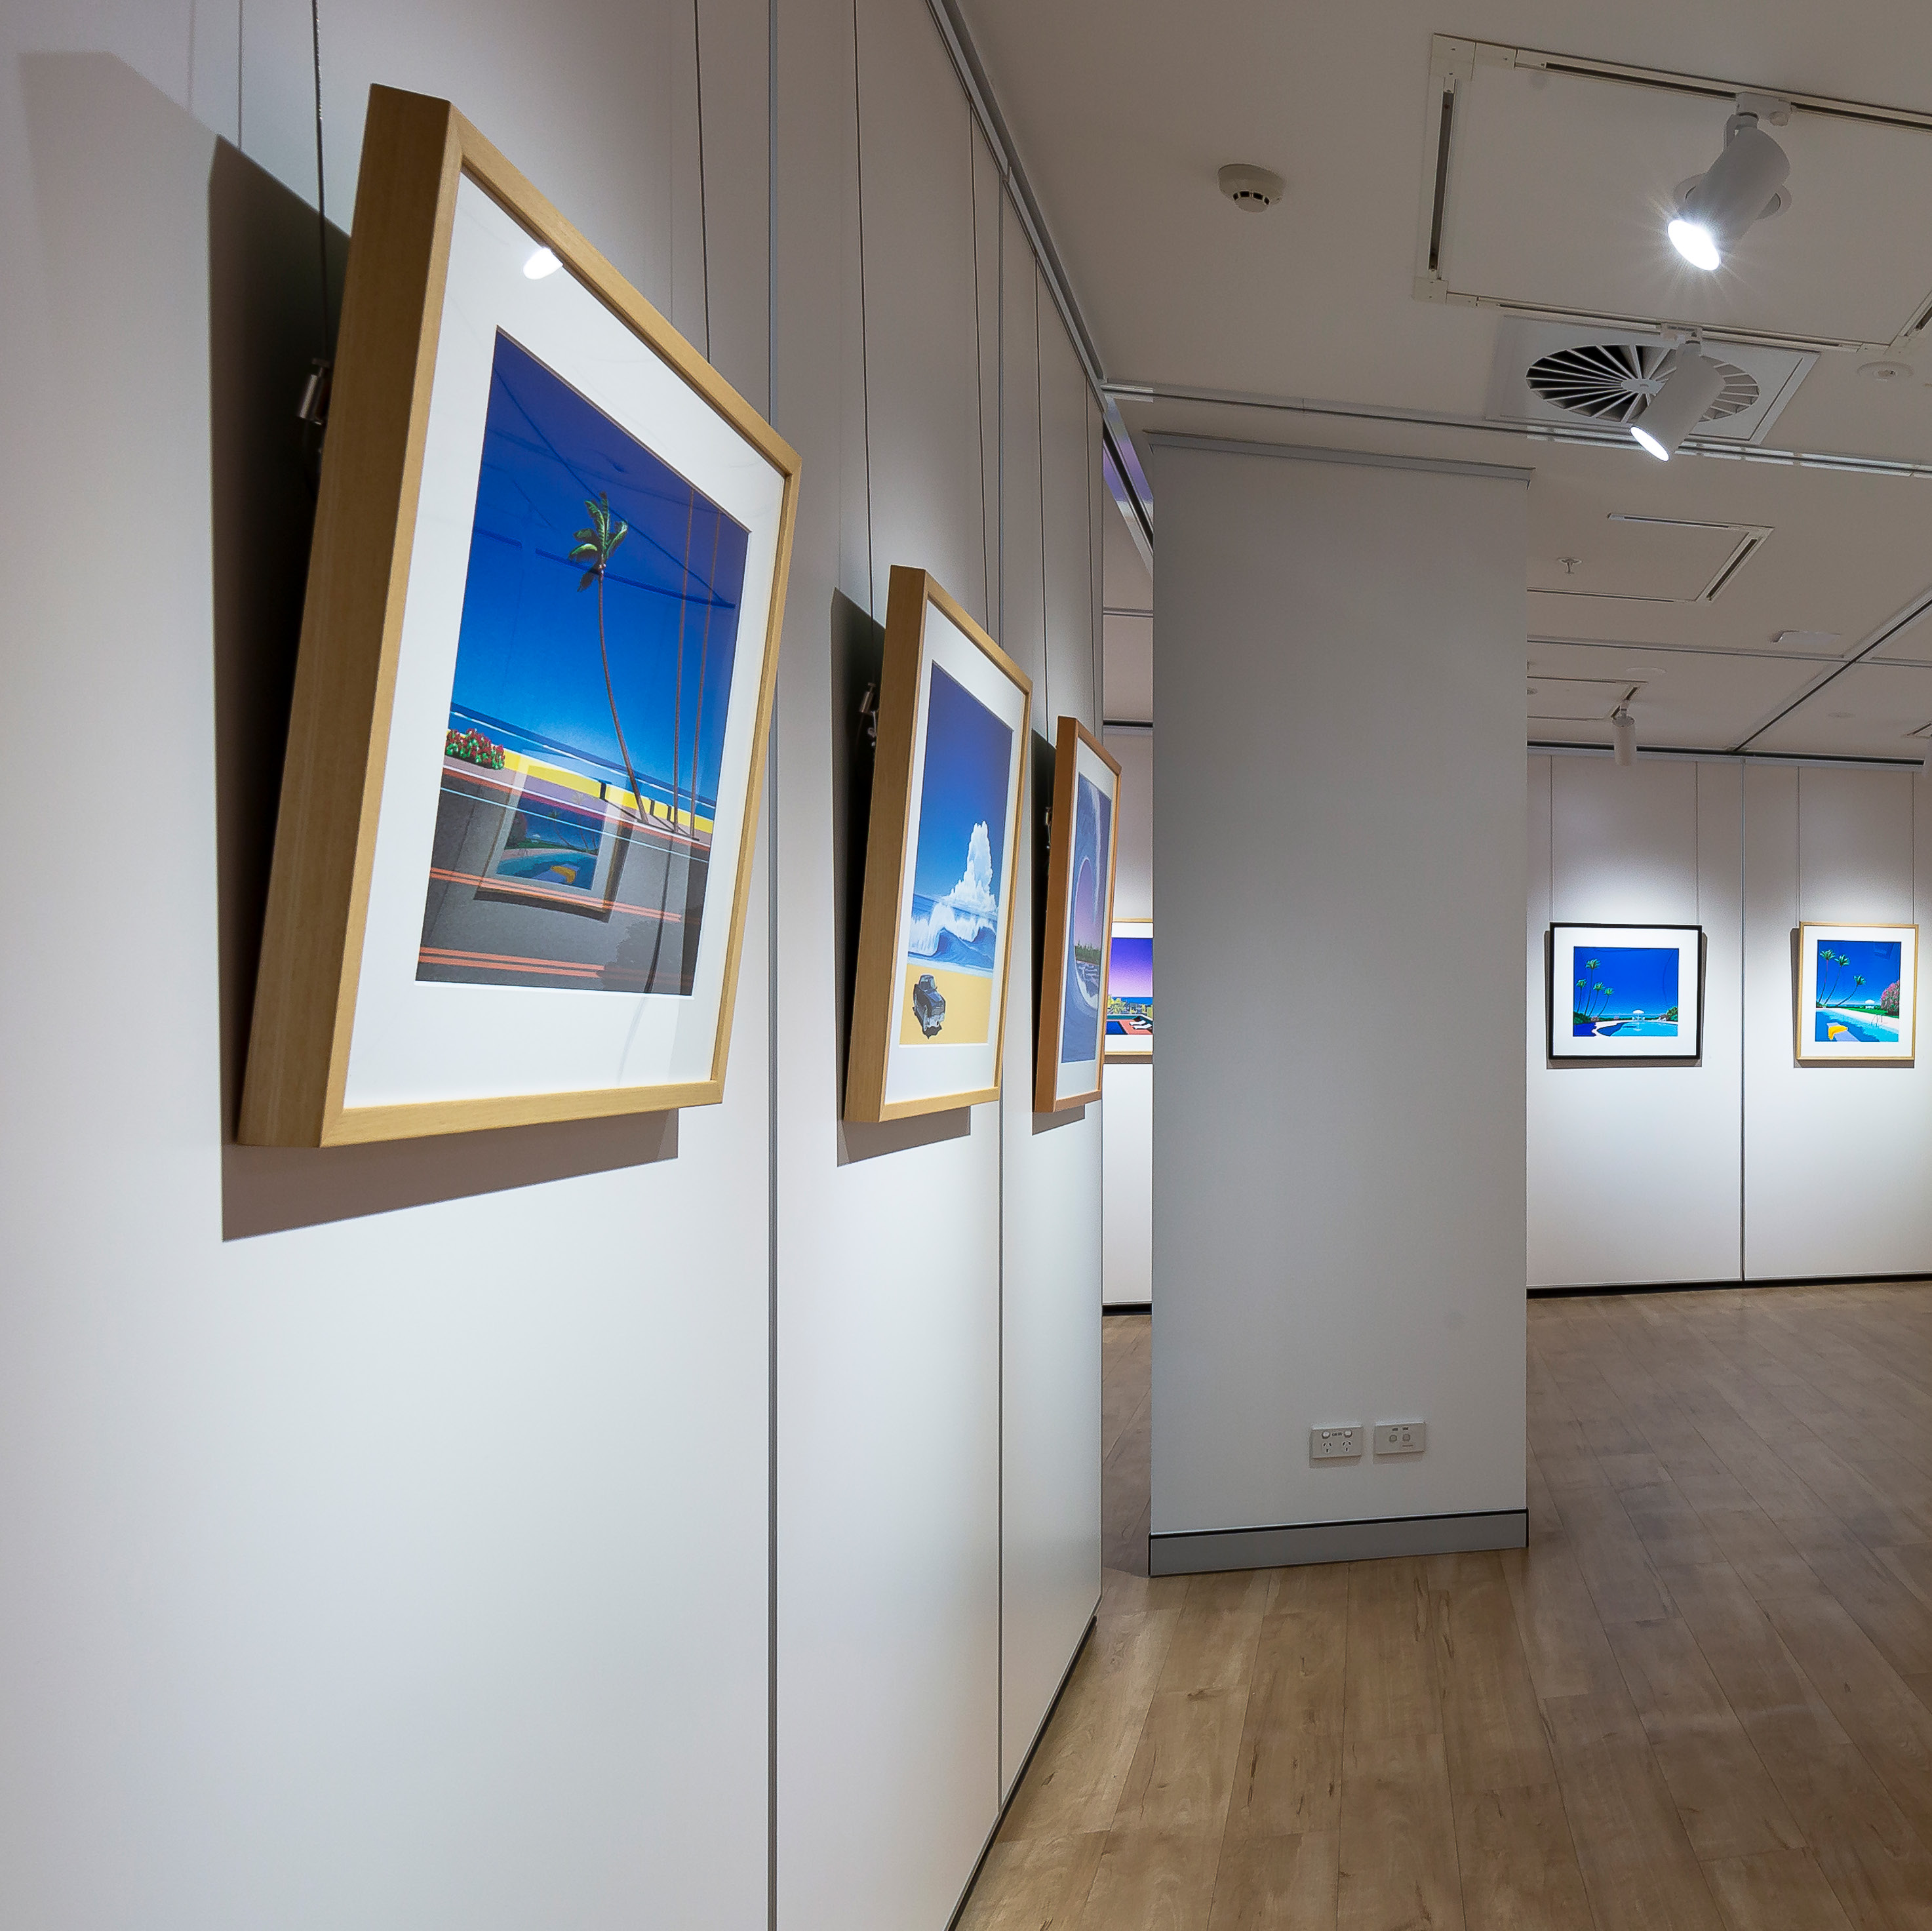
\includegraphics[width=0.52083in,height=\textheight,keepaspectratio]{img/jpf/9.jpg}
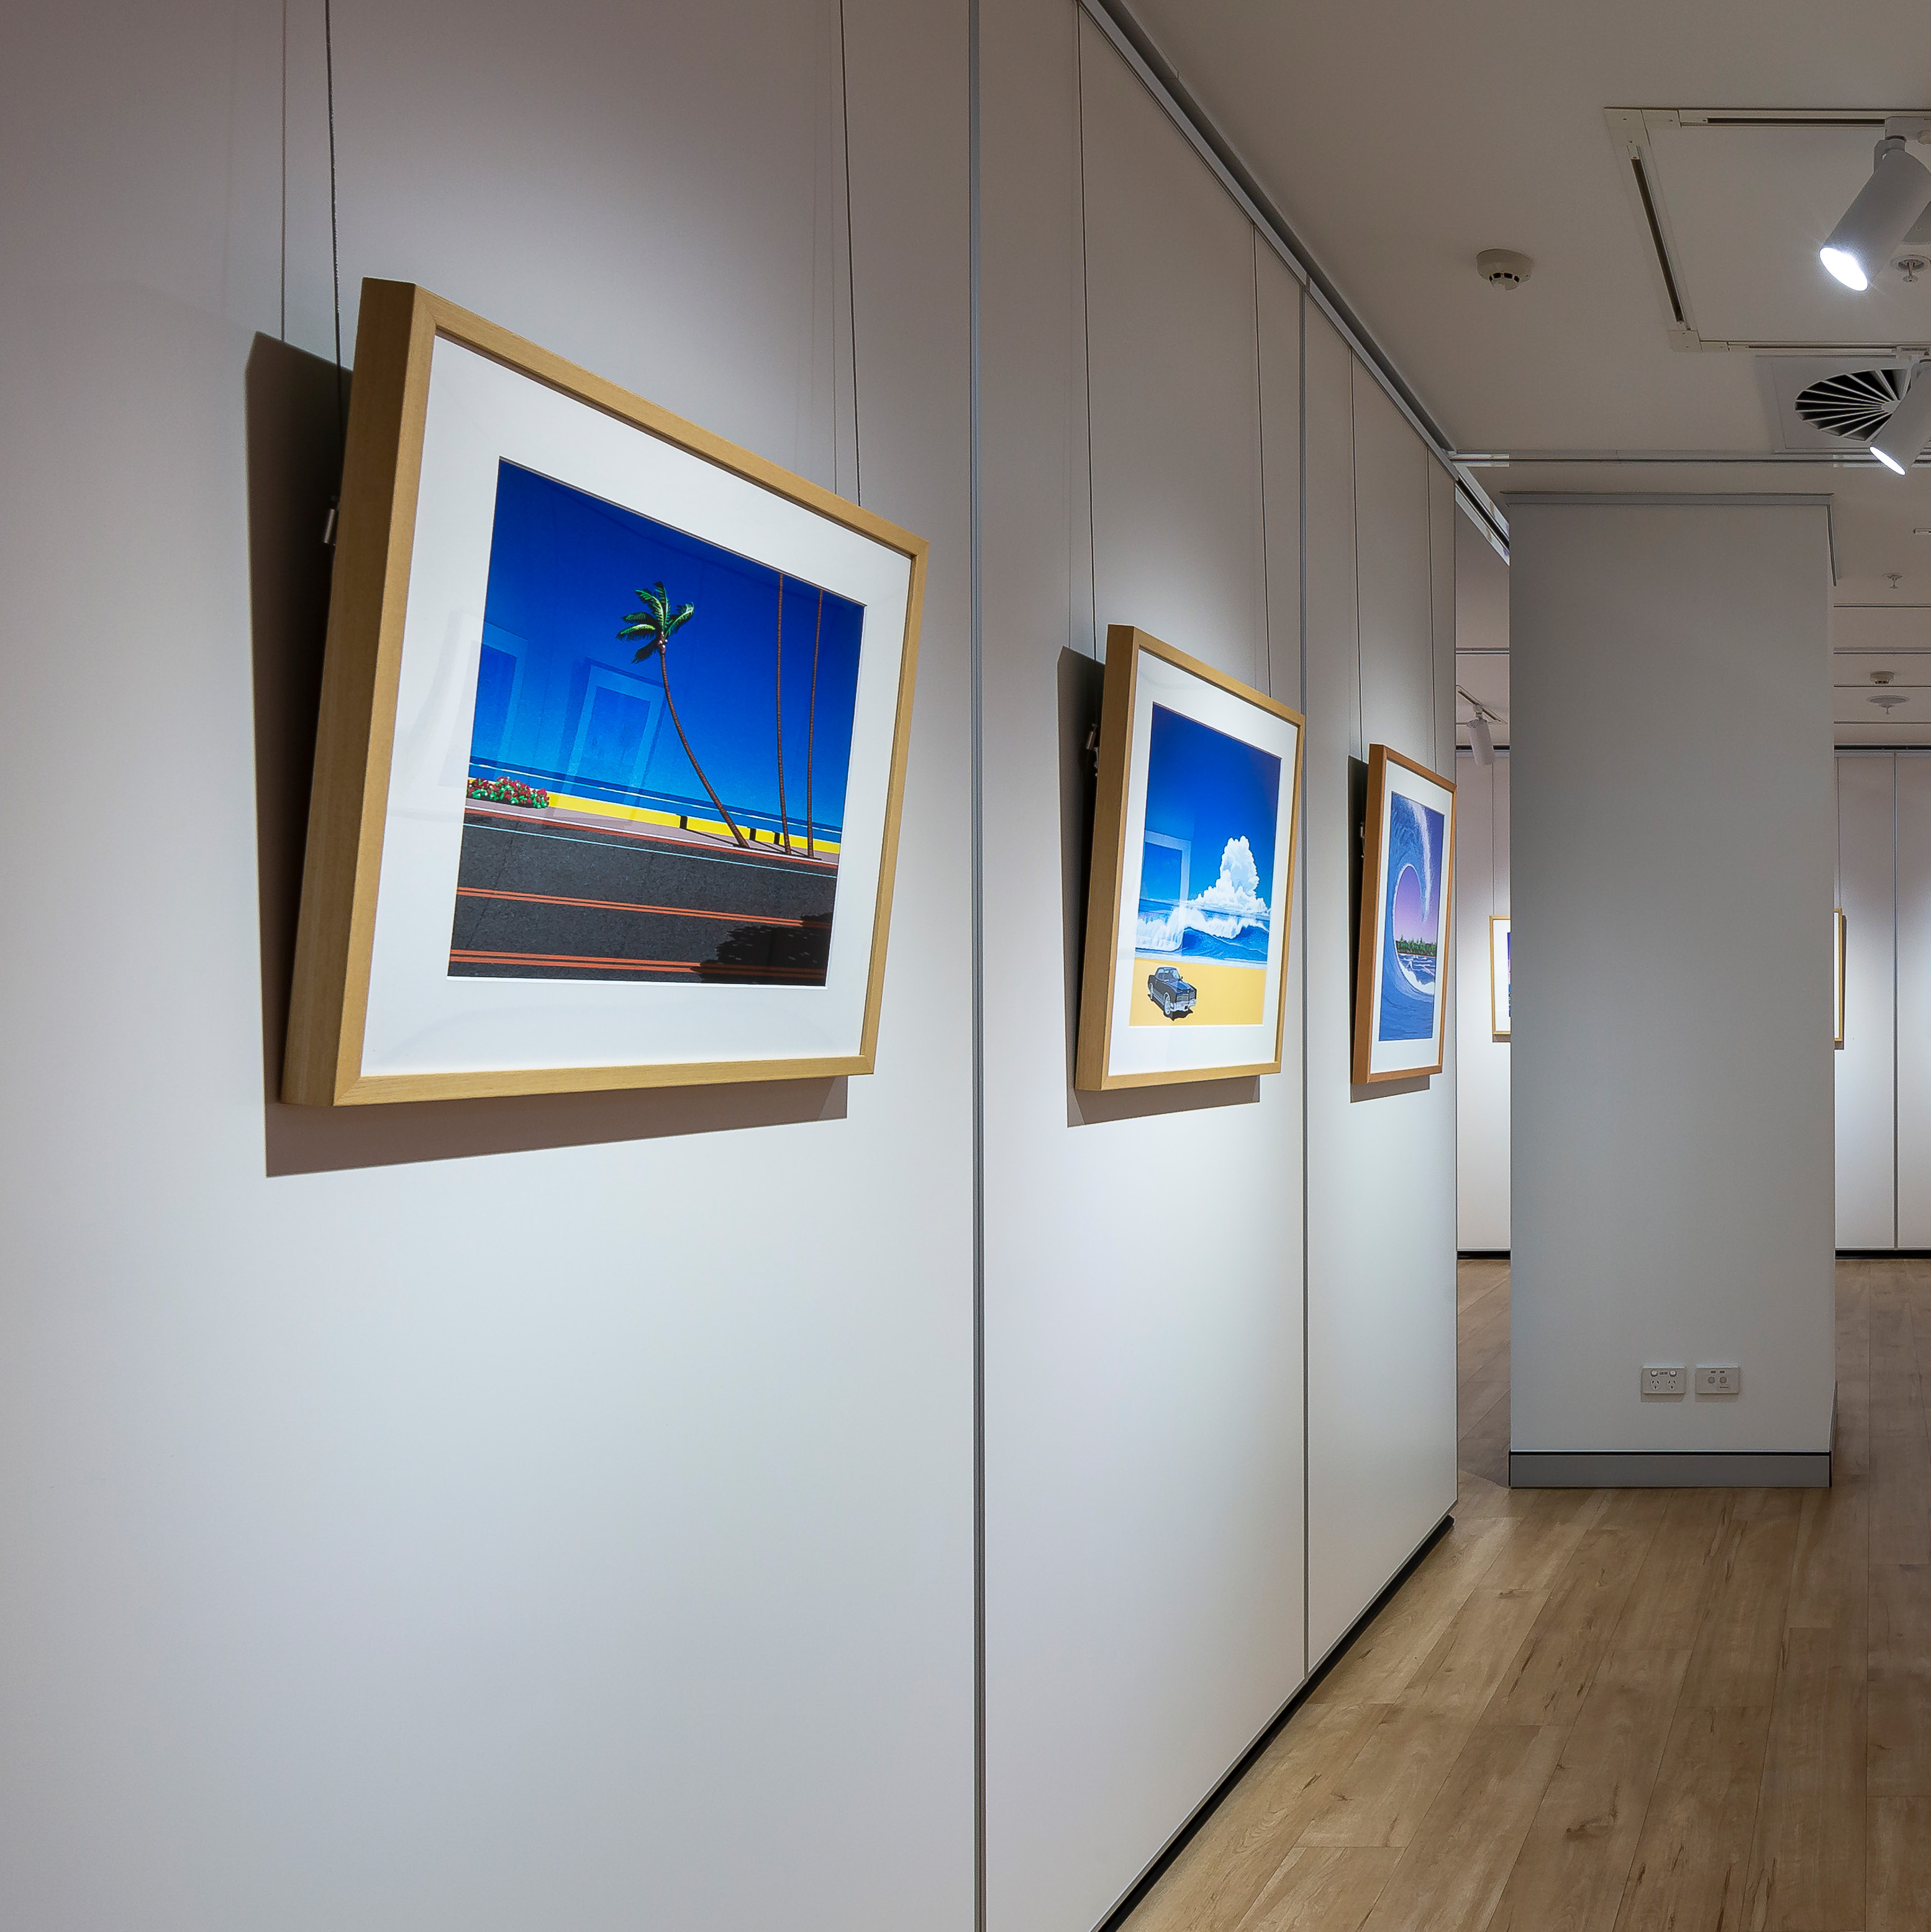
\includegraphics[width=0.52083in,height=\textheight,keepaspectratio]{img/jpf/10.jpg}
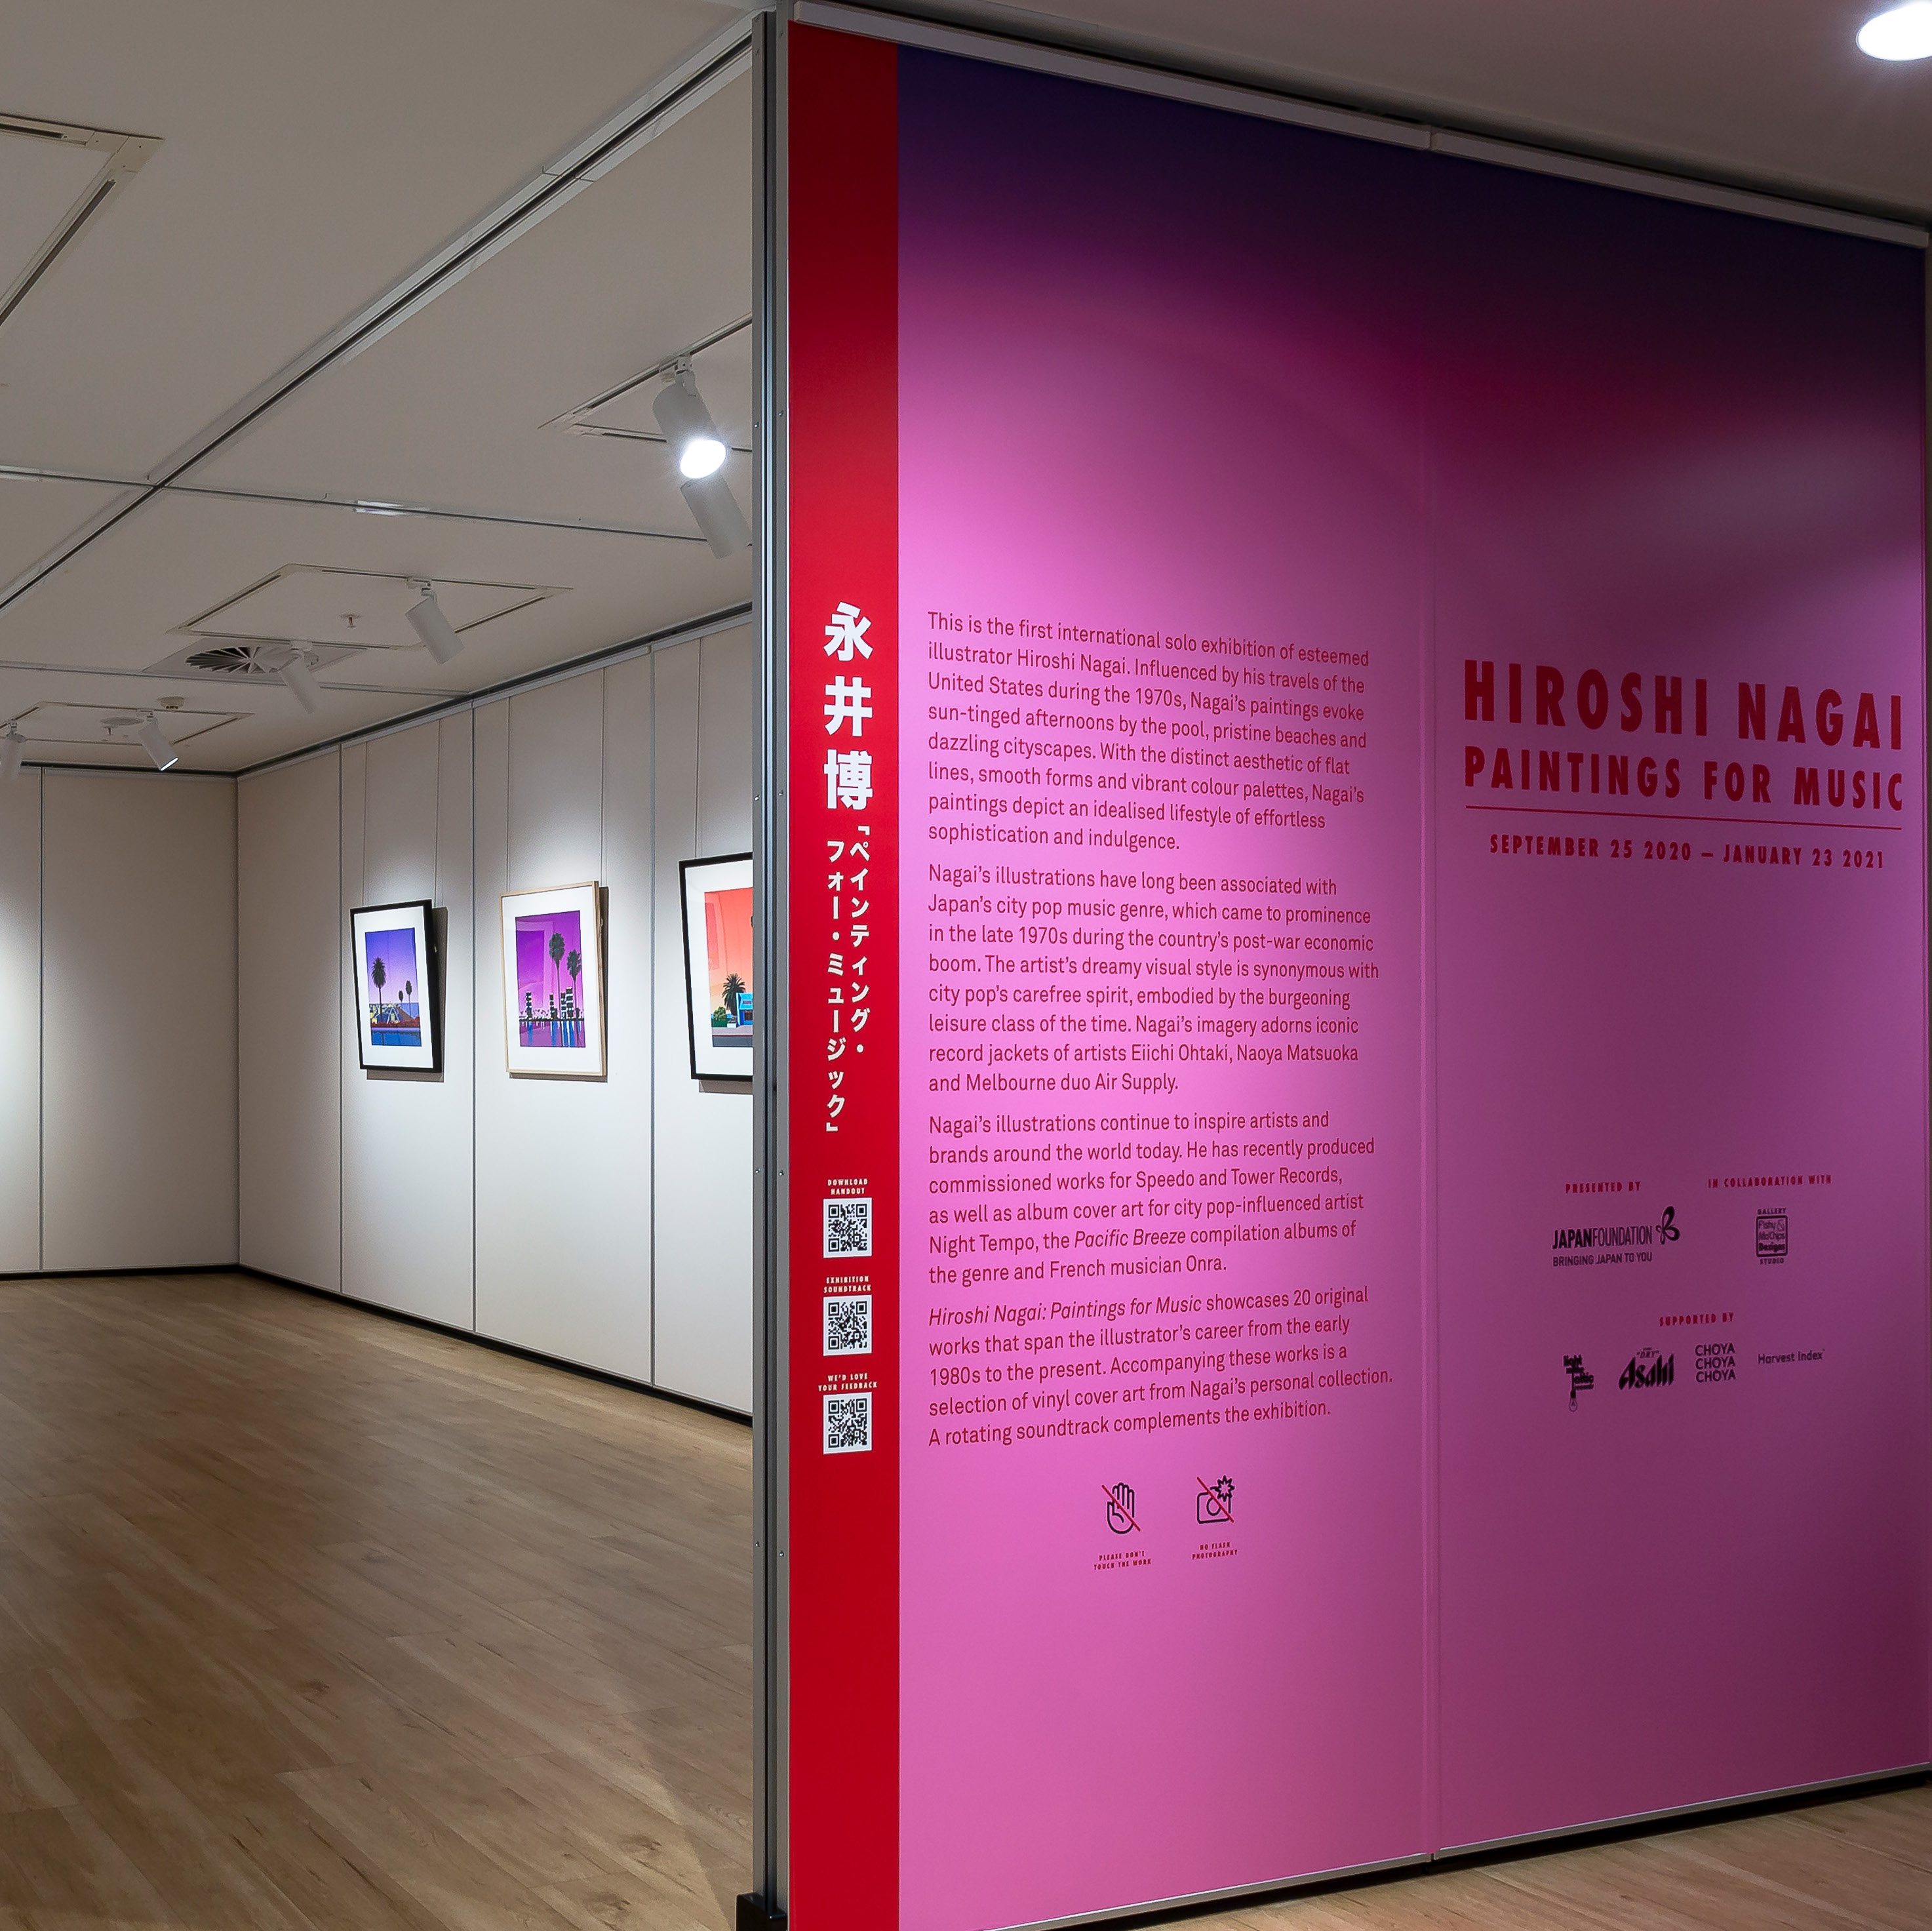
\includegraphics[width=0.52083in,height=\textheight,keepaspectratio]{img/jpf/11.jpg}
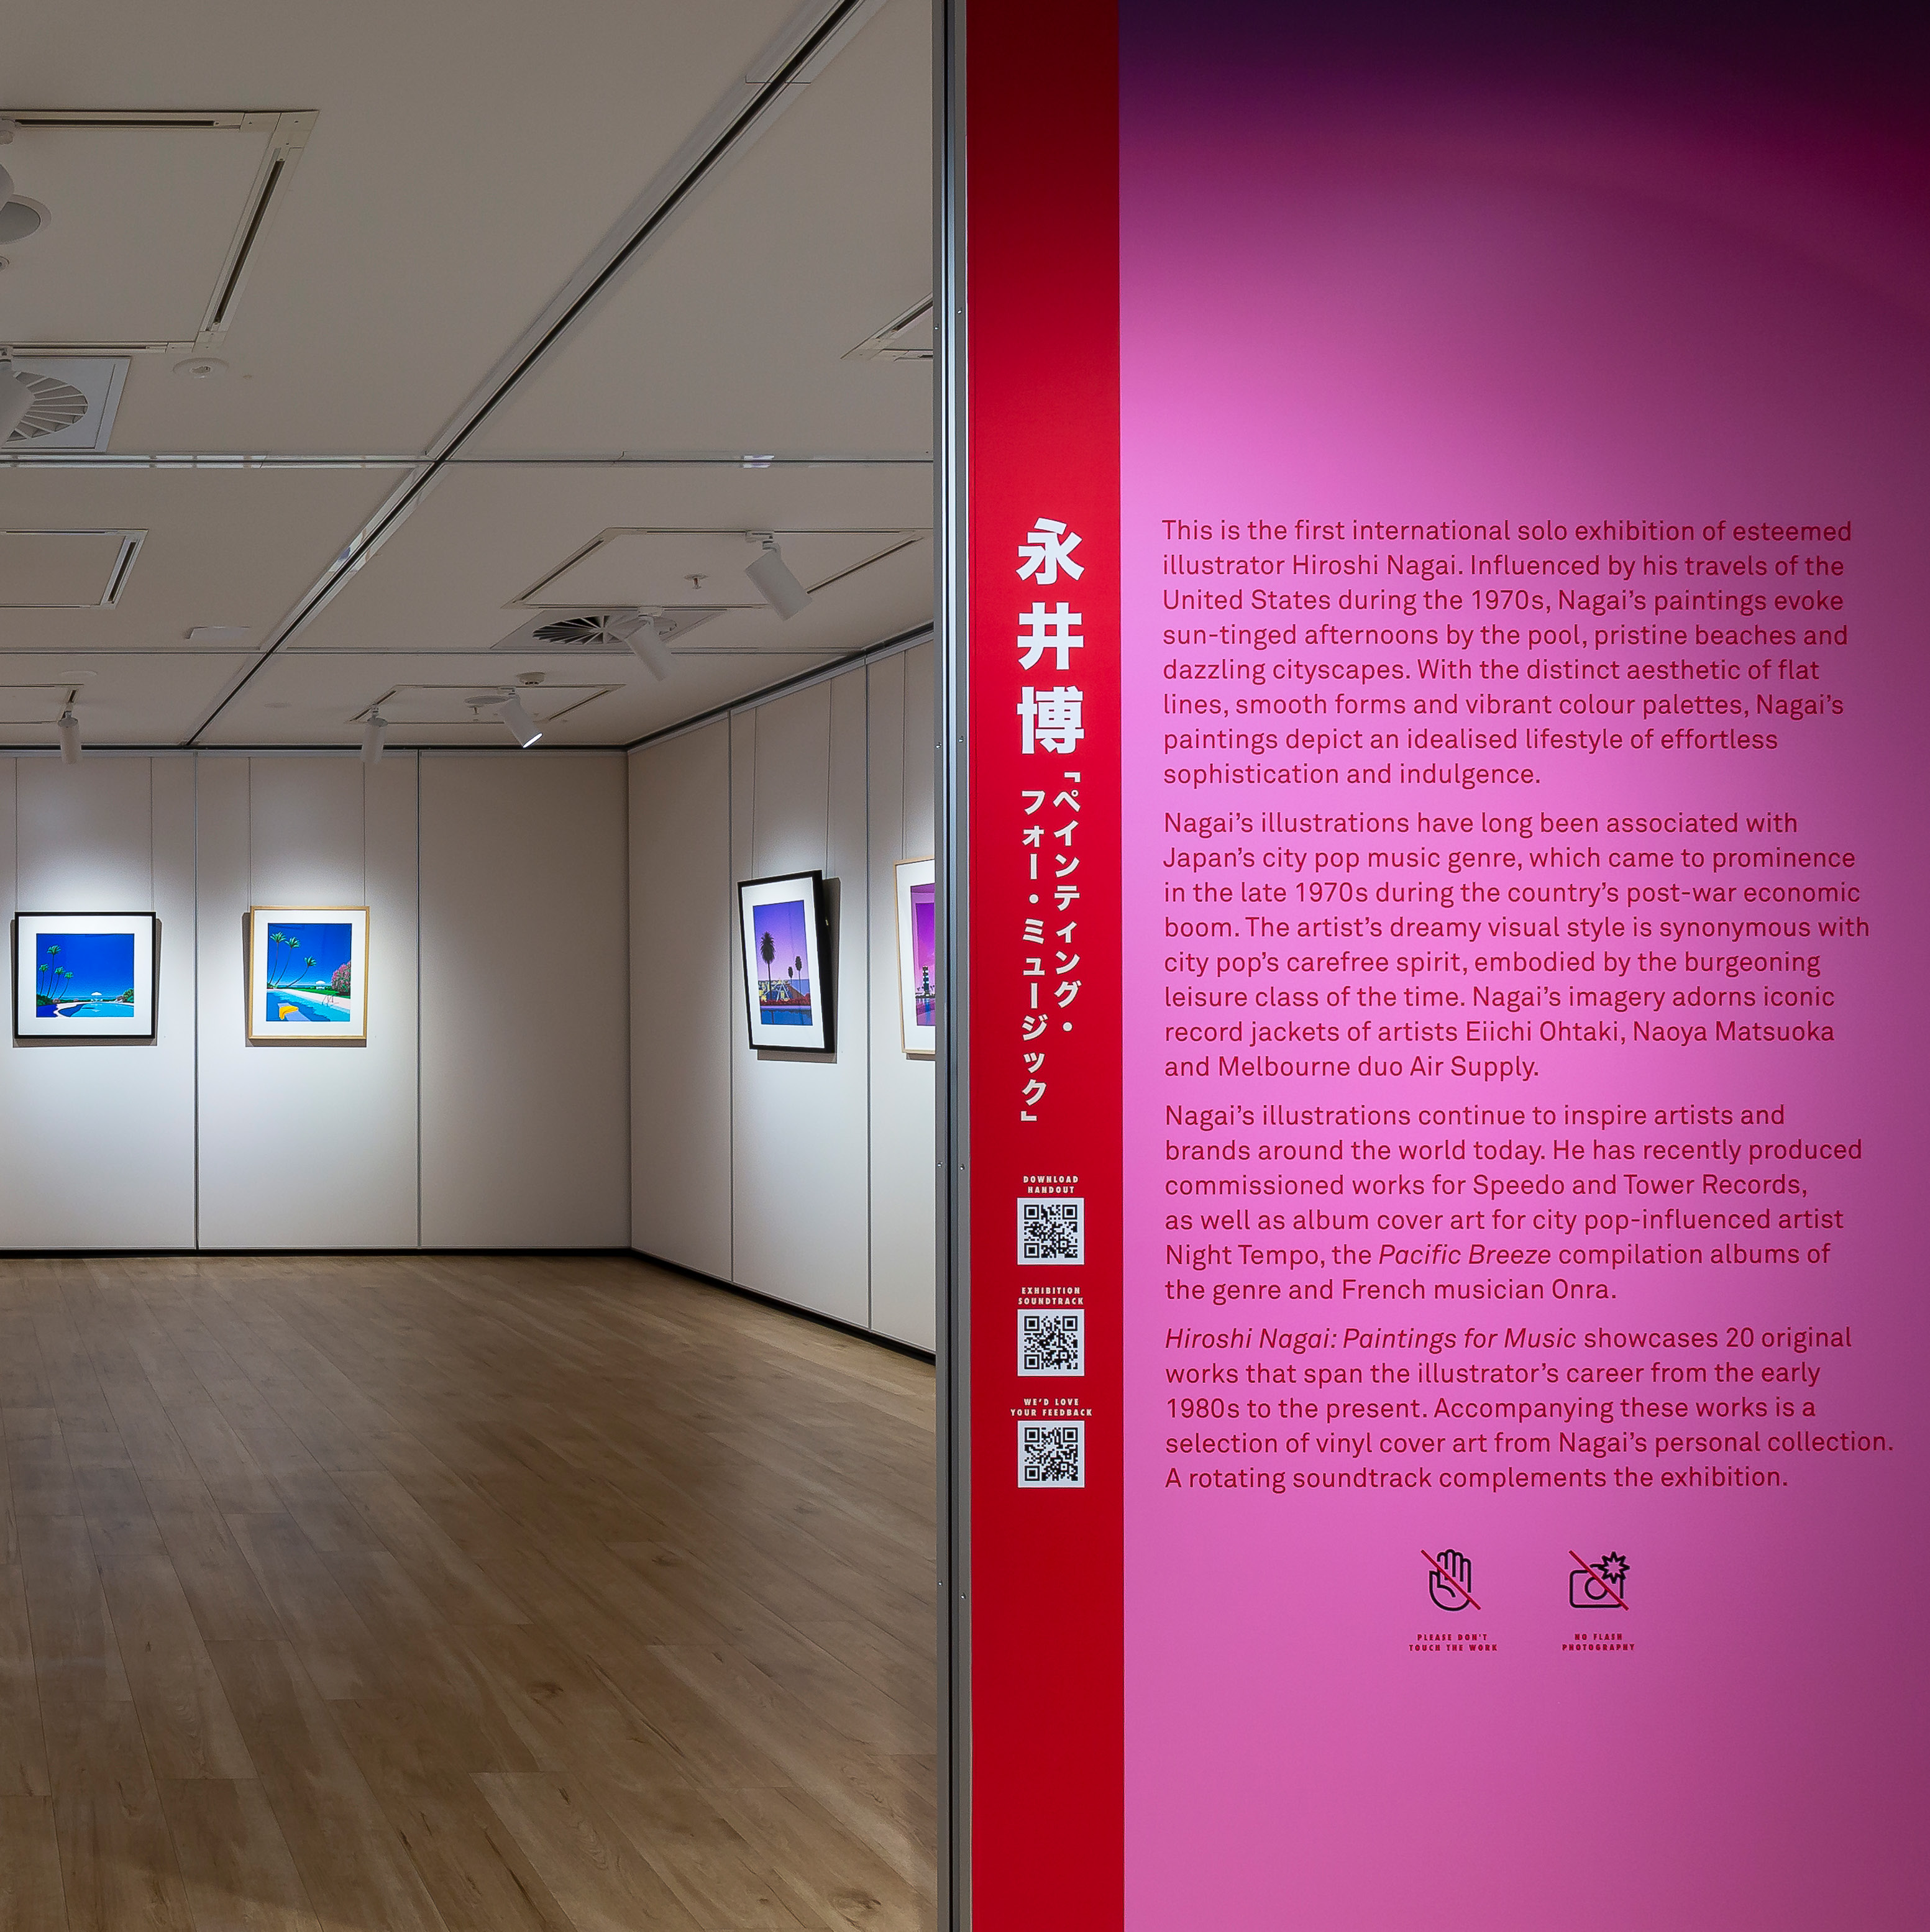
\includegraphics[width=0.52083in,height=\textheight,keepaspectratio]{img/jpf/12.jpg}
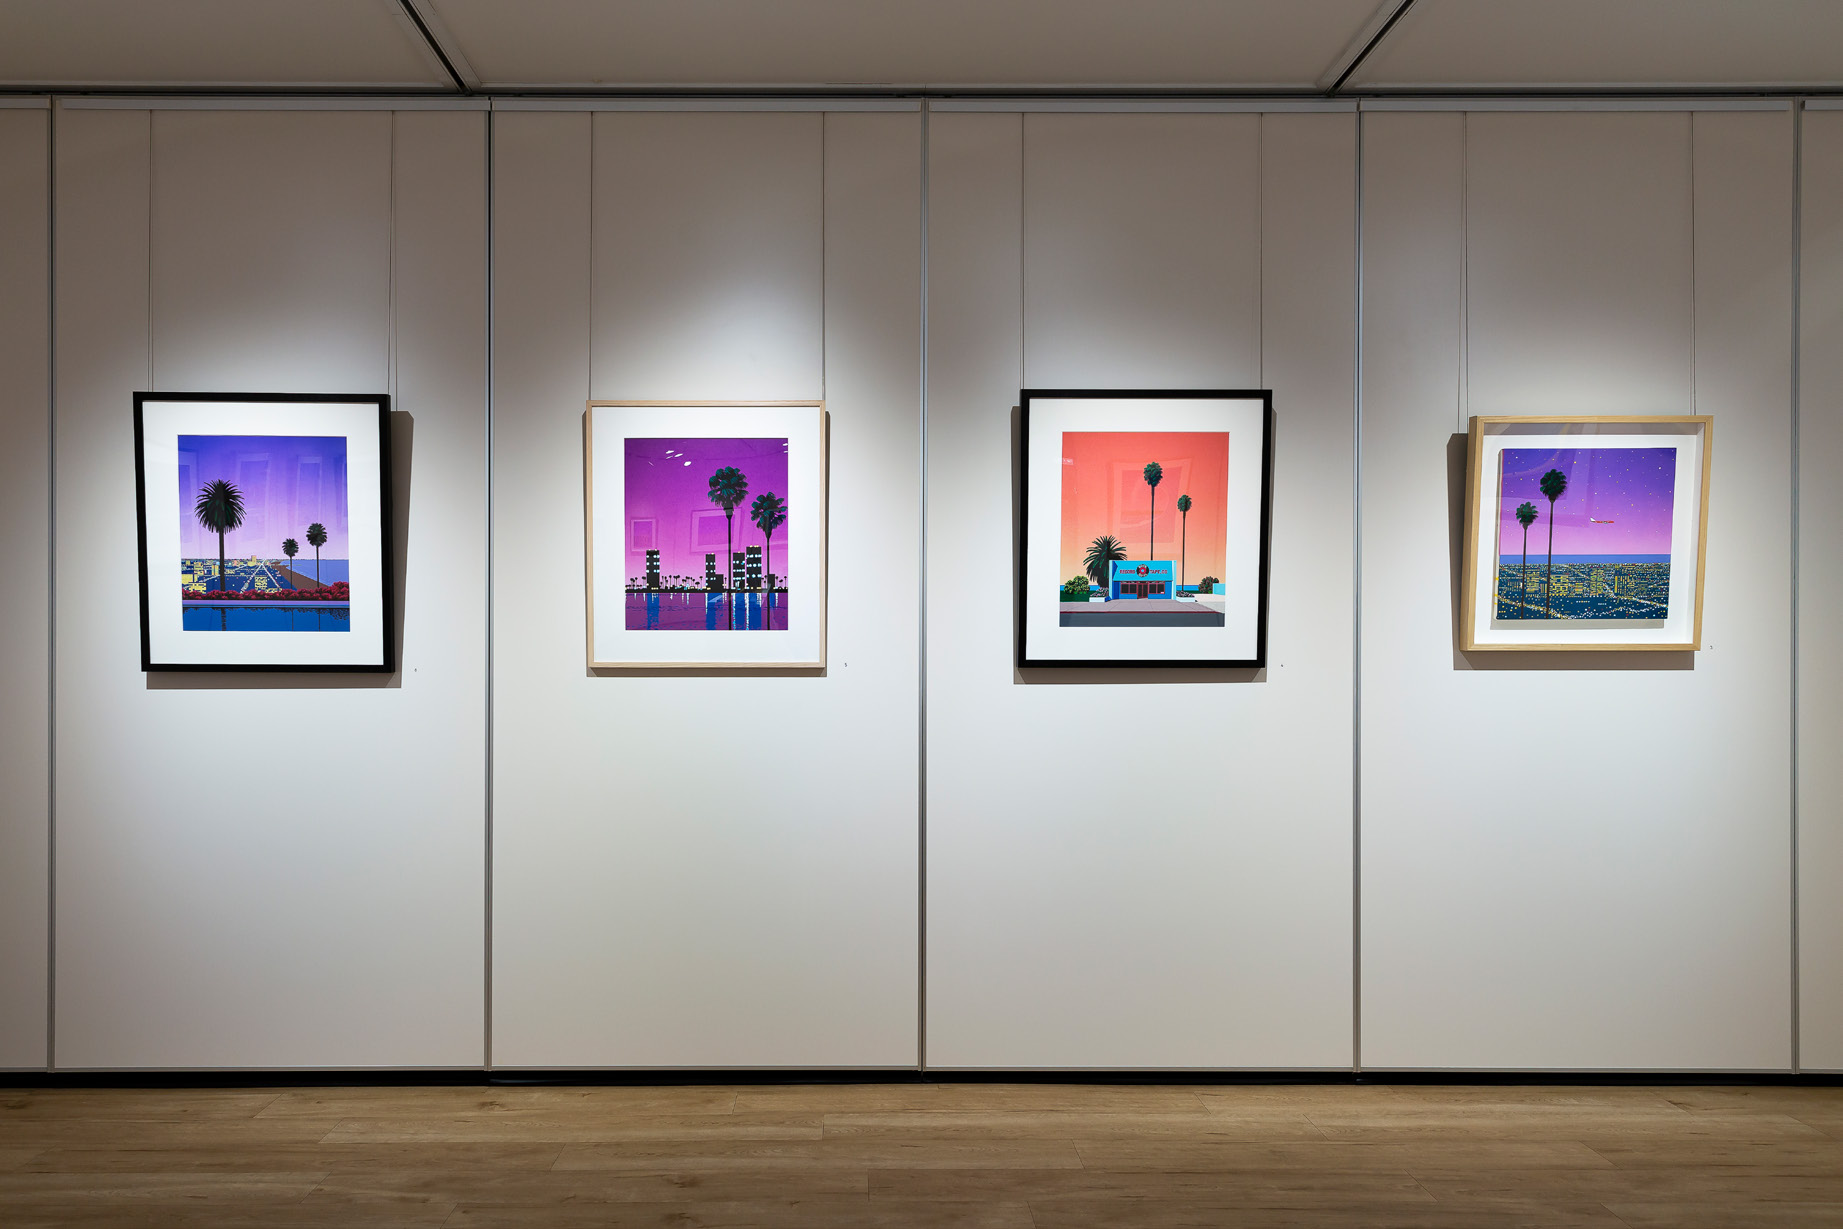
\includegraphics[width=0.52083in,height=\textheight,keepaspectratio]{img/jpf/13.jpg}
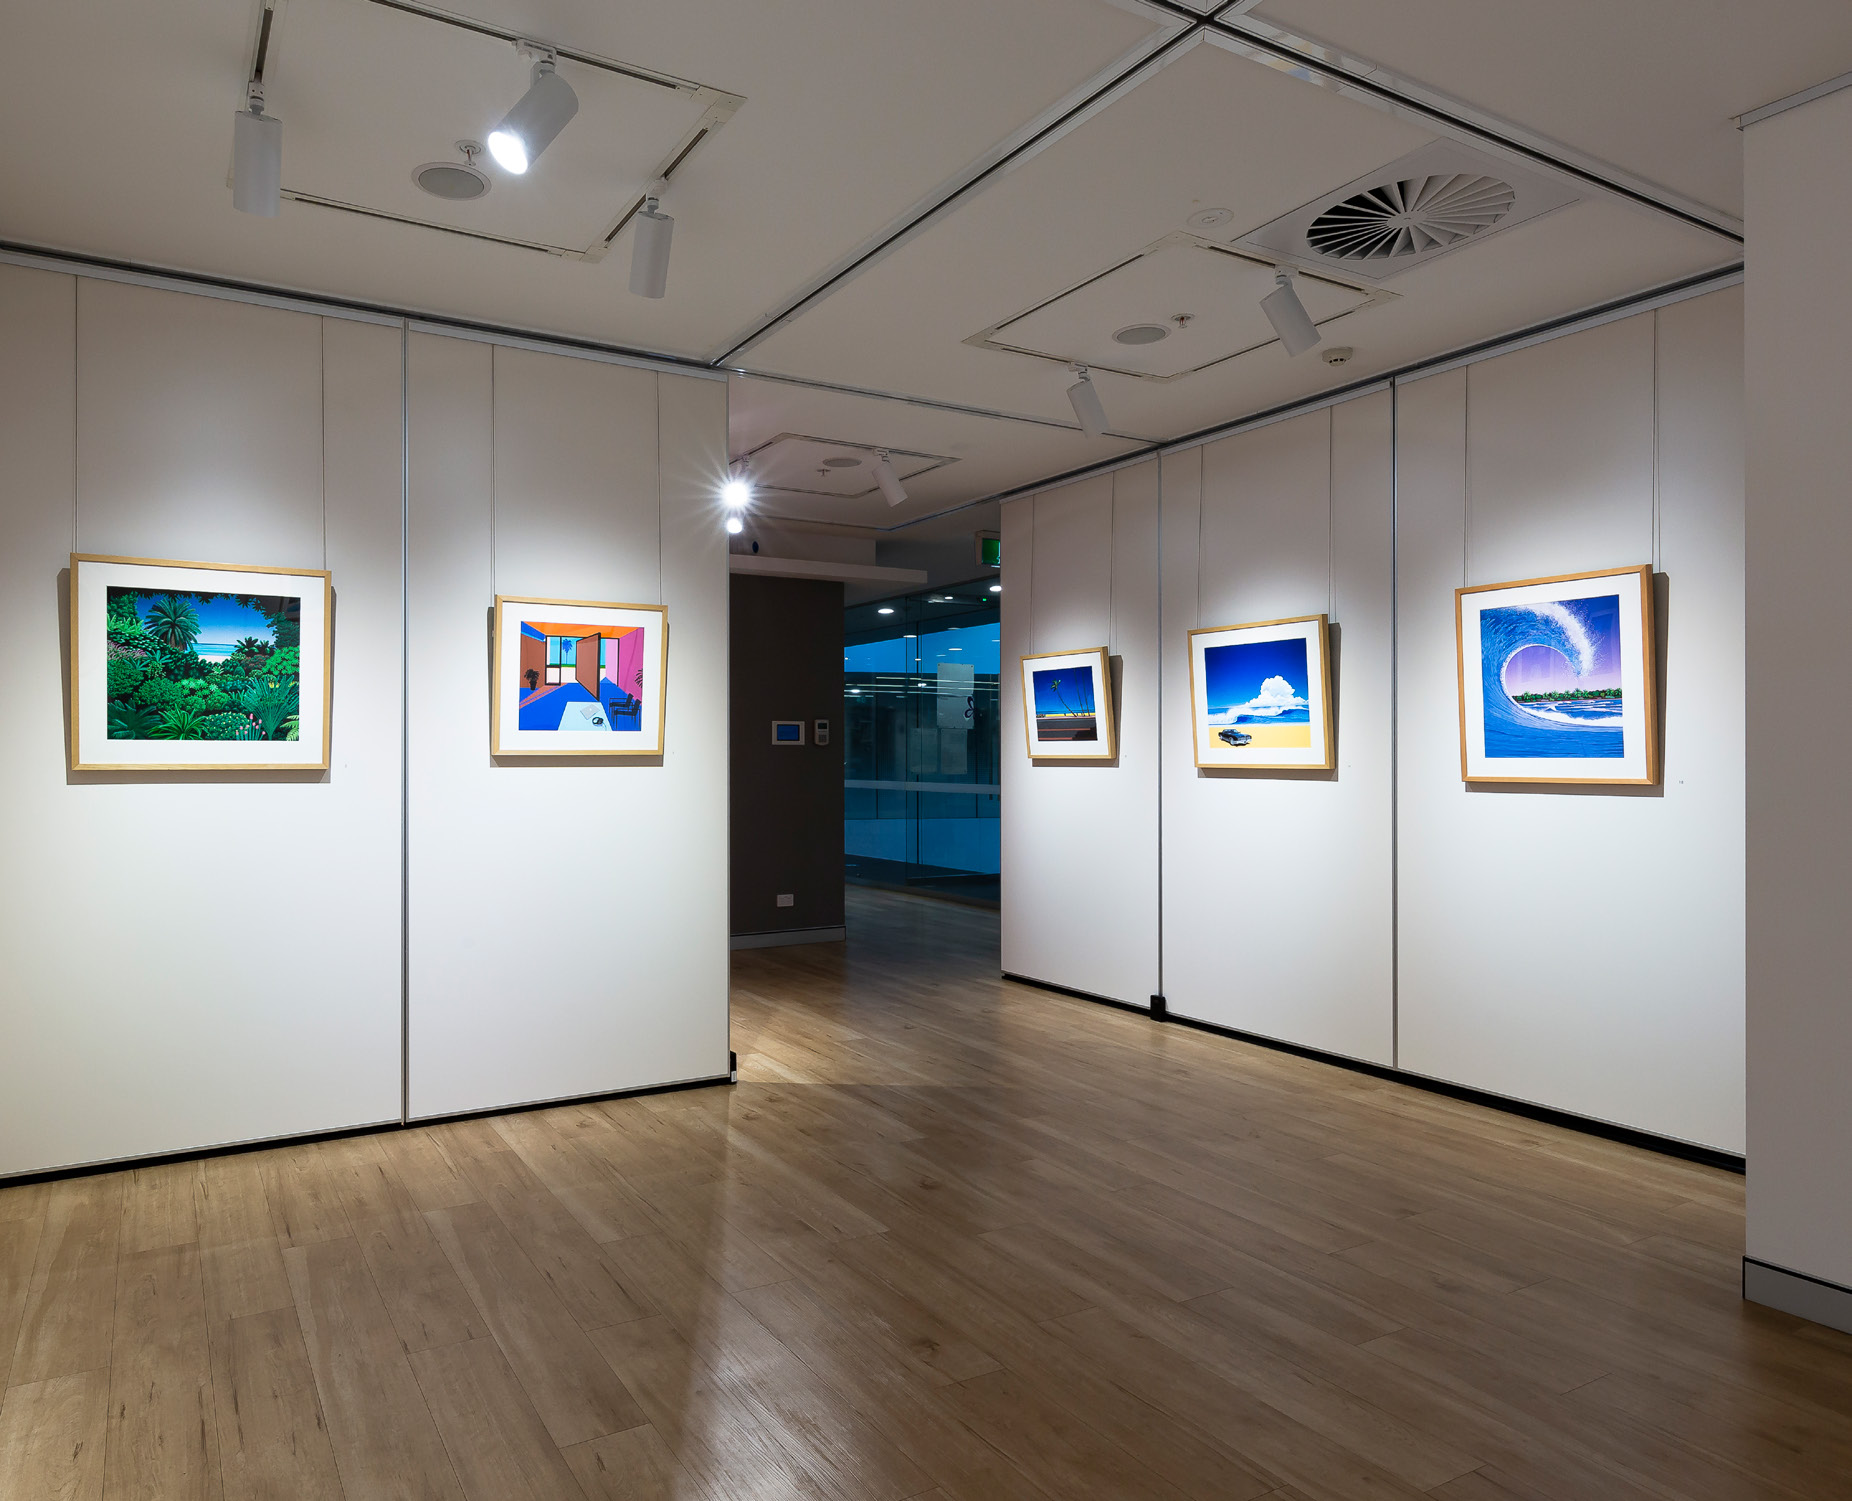
\includegraphics[width=0.52083in,height=\textheight,keepaspectratio]{img/jpf/14.jpg}
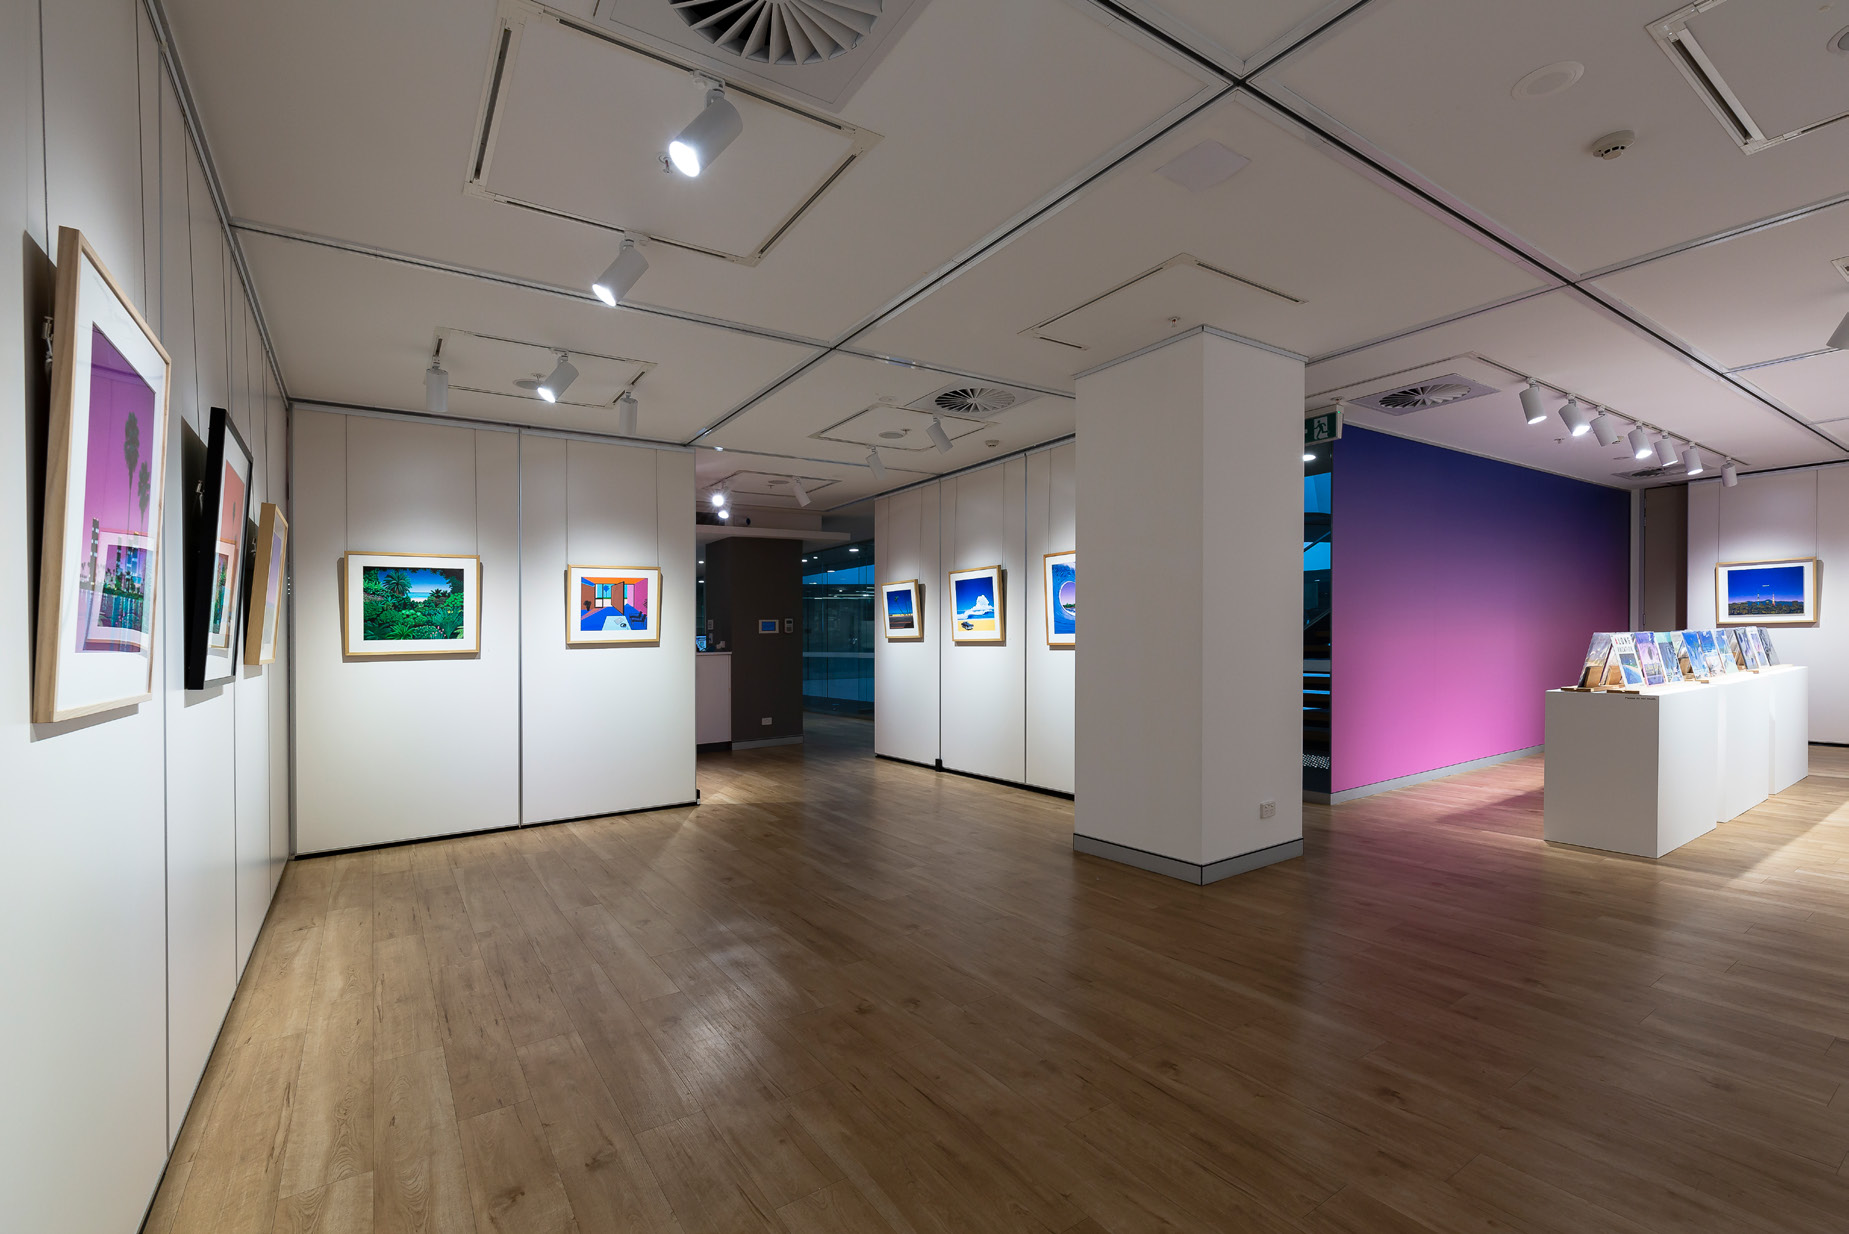
\includegraphics[width=0.52083in,height=\textheight,keepaspectratio]{img/jpf/15.jpg}
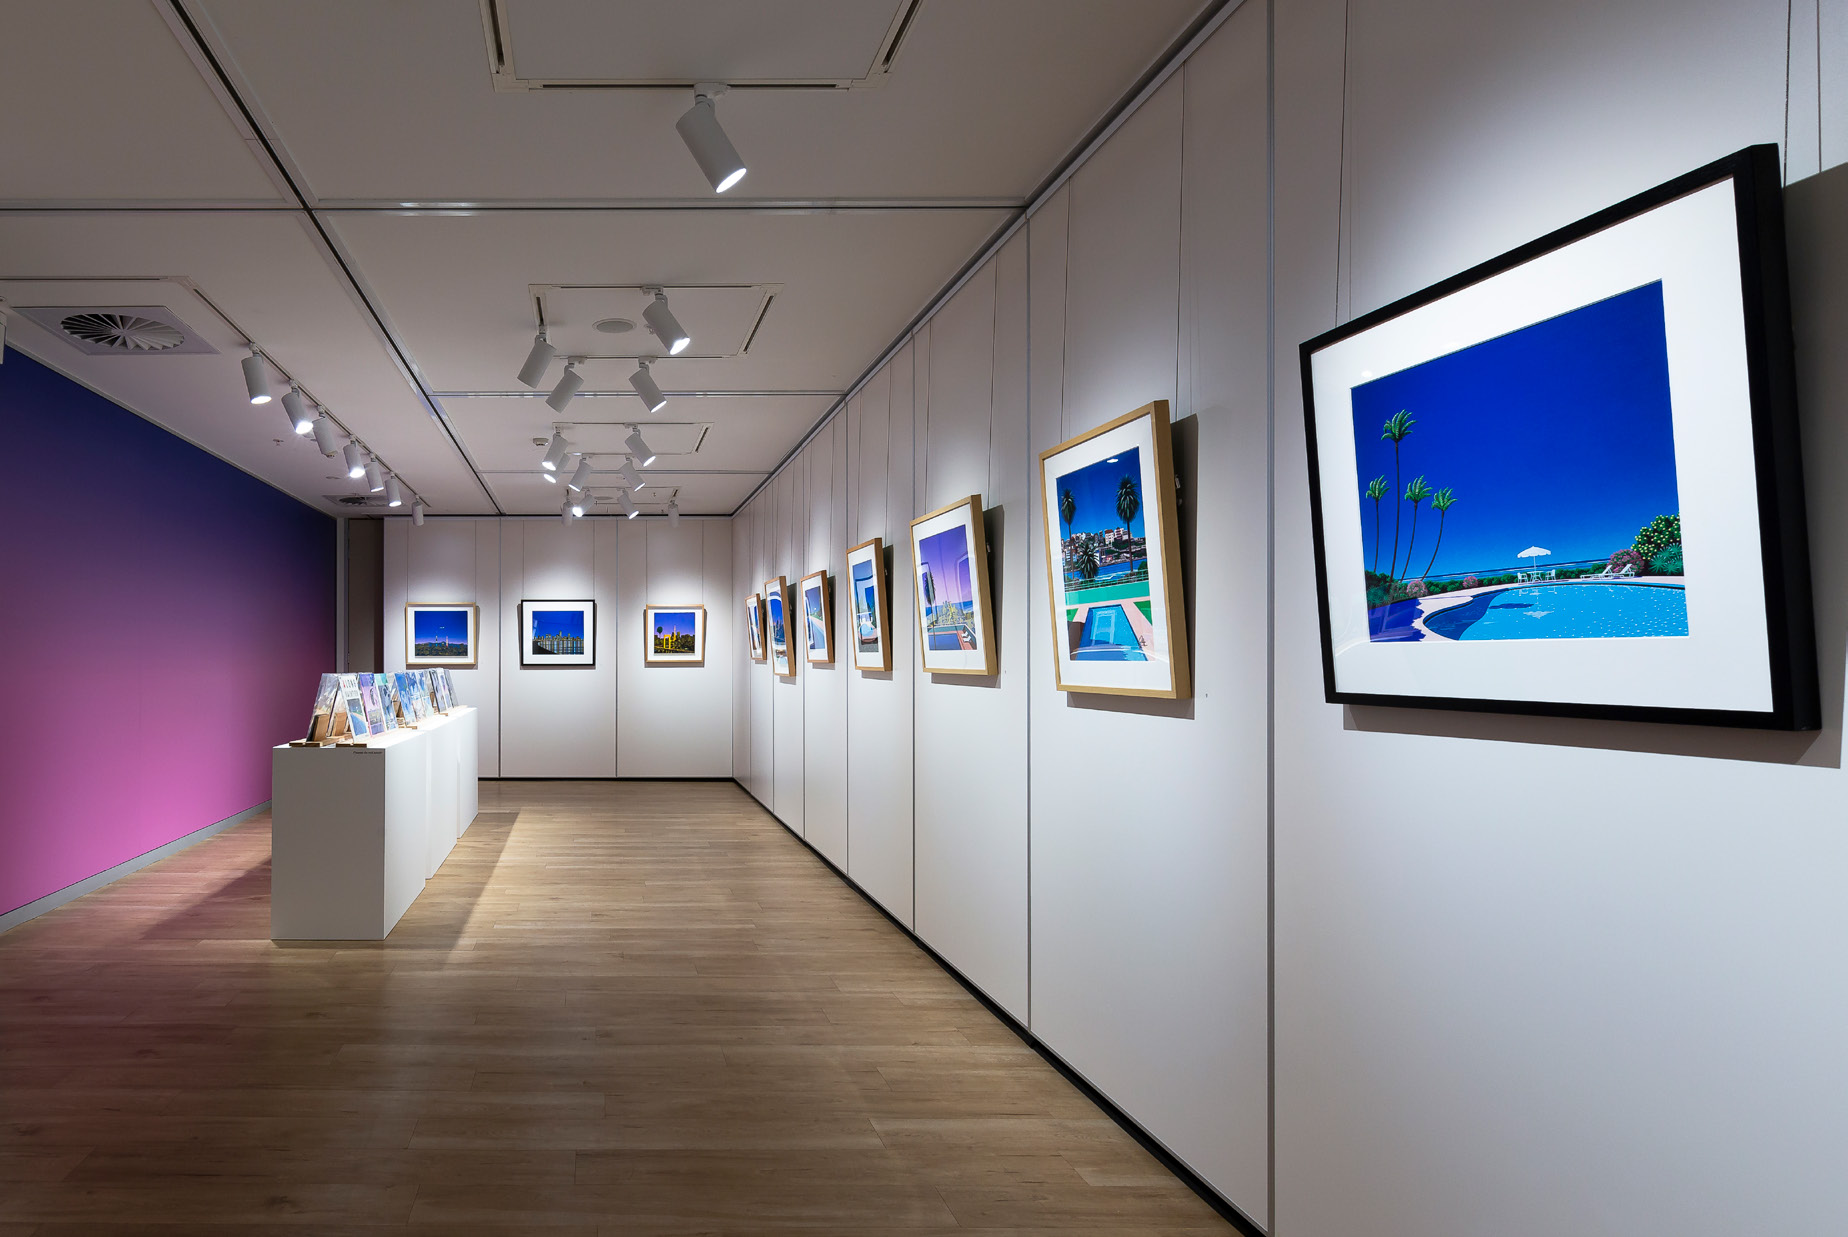
\includegraphics[width=0.52083in,height=\textheight,keepaspectratio]{img/jpf/16.jpg}
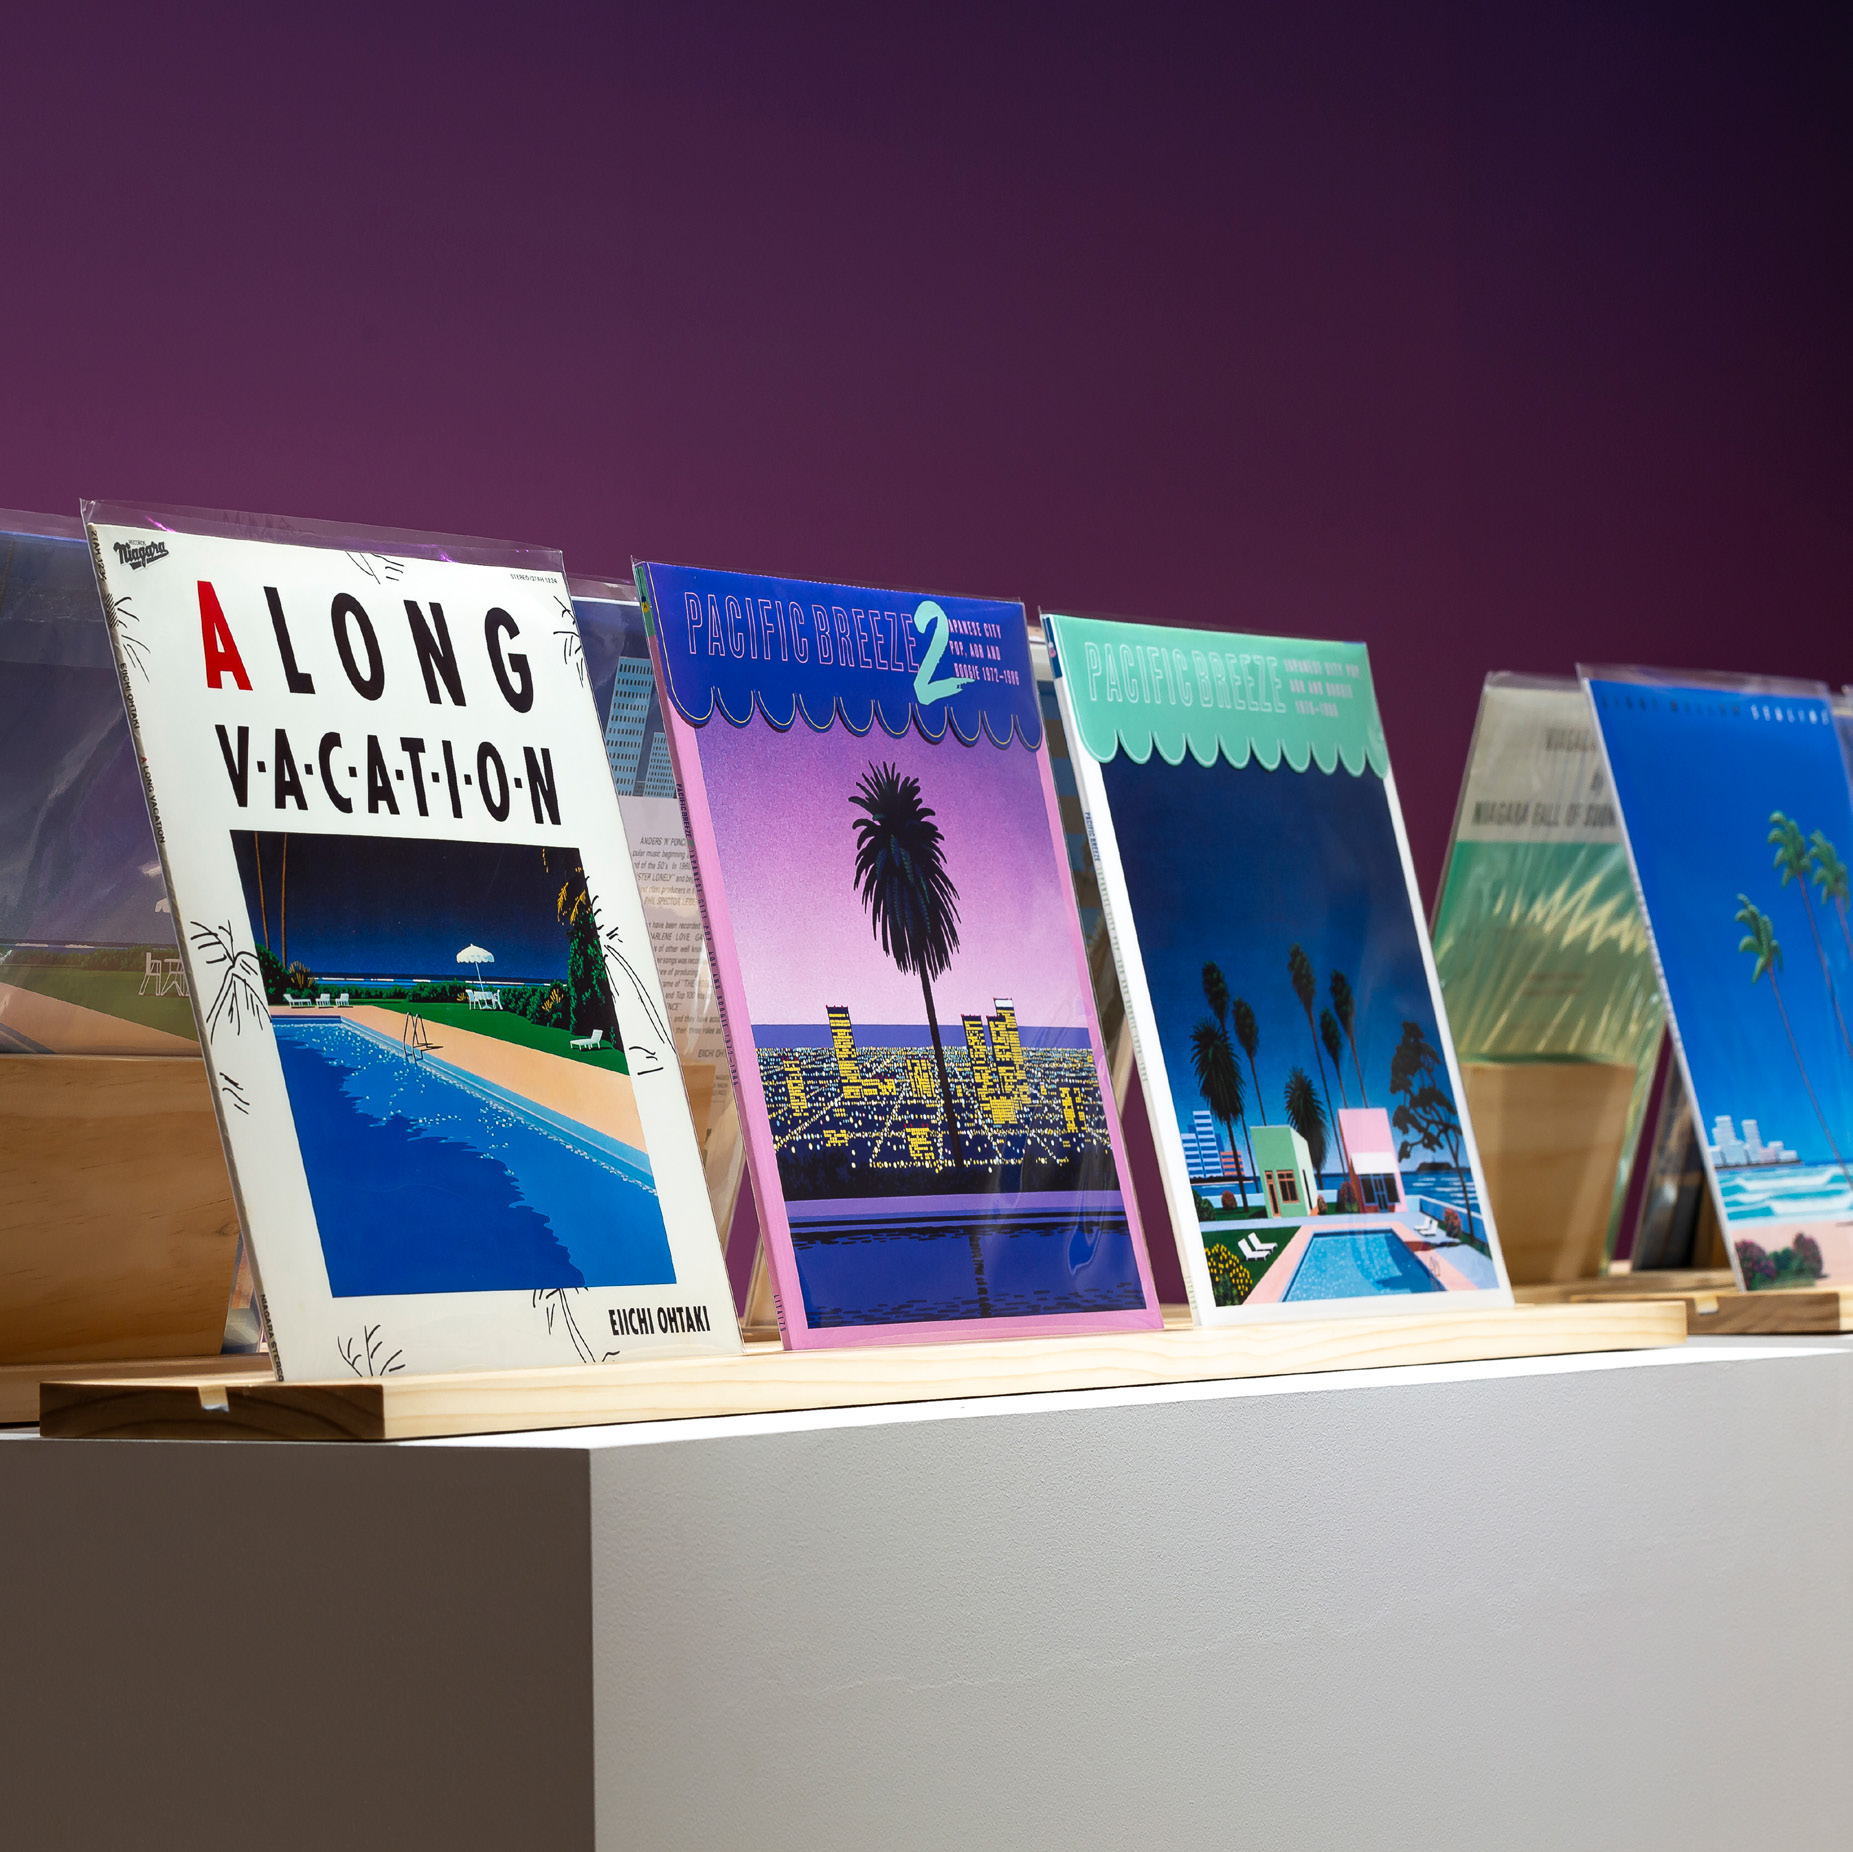
\includegraphics[width=0.52083in,height=\textheight,keepaspectratio]{img/jpf/17.jpg}
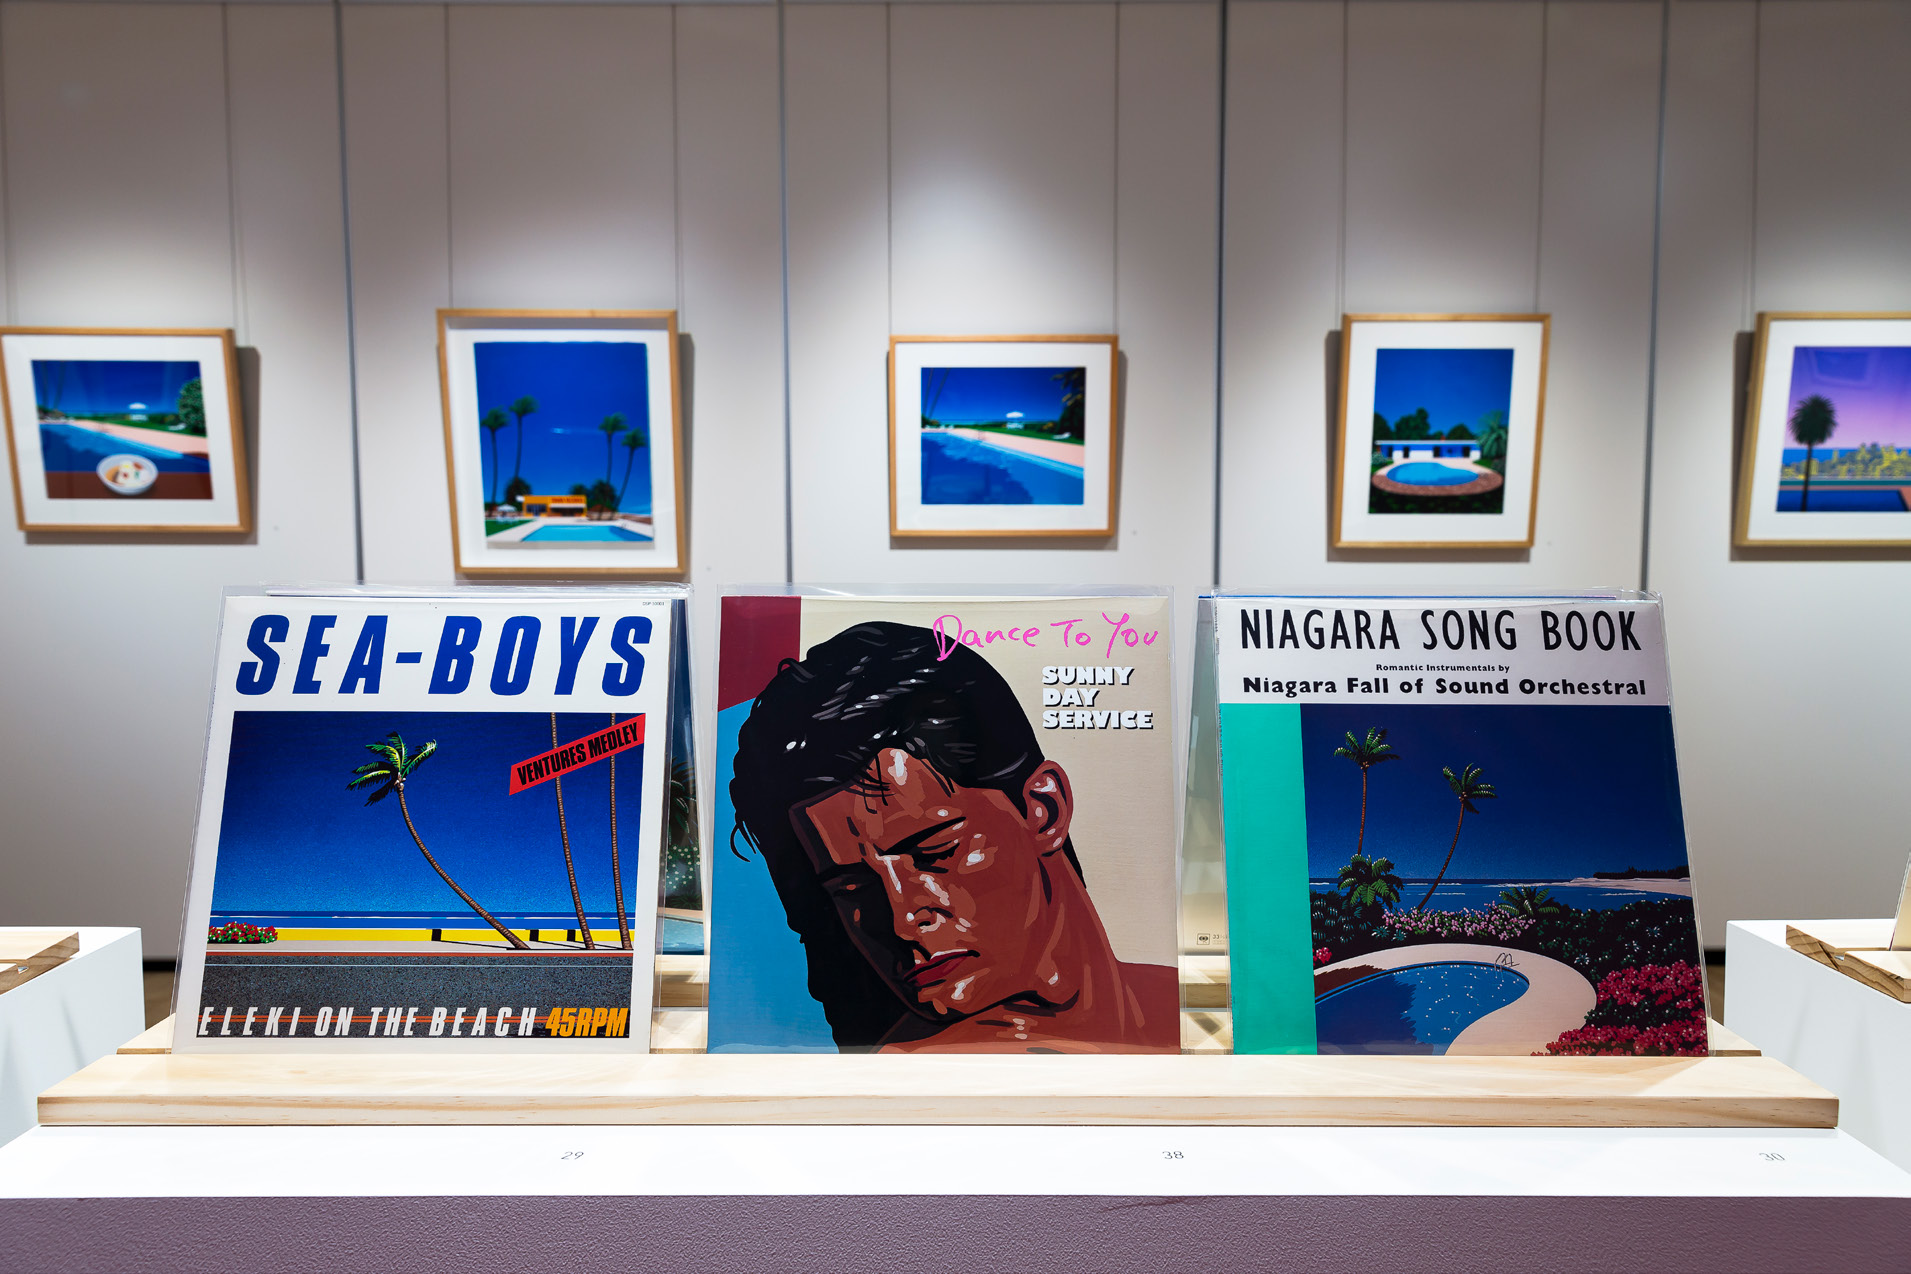
\includegraphics[width=0.52083in,height=\textheight,keepaspectratio]{img/jpf/18.jpg}
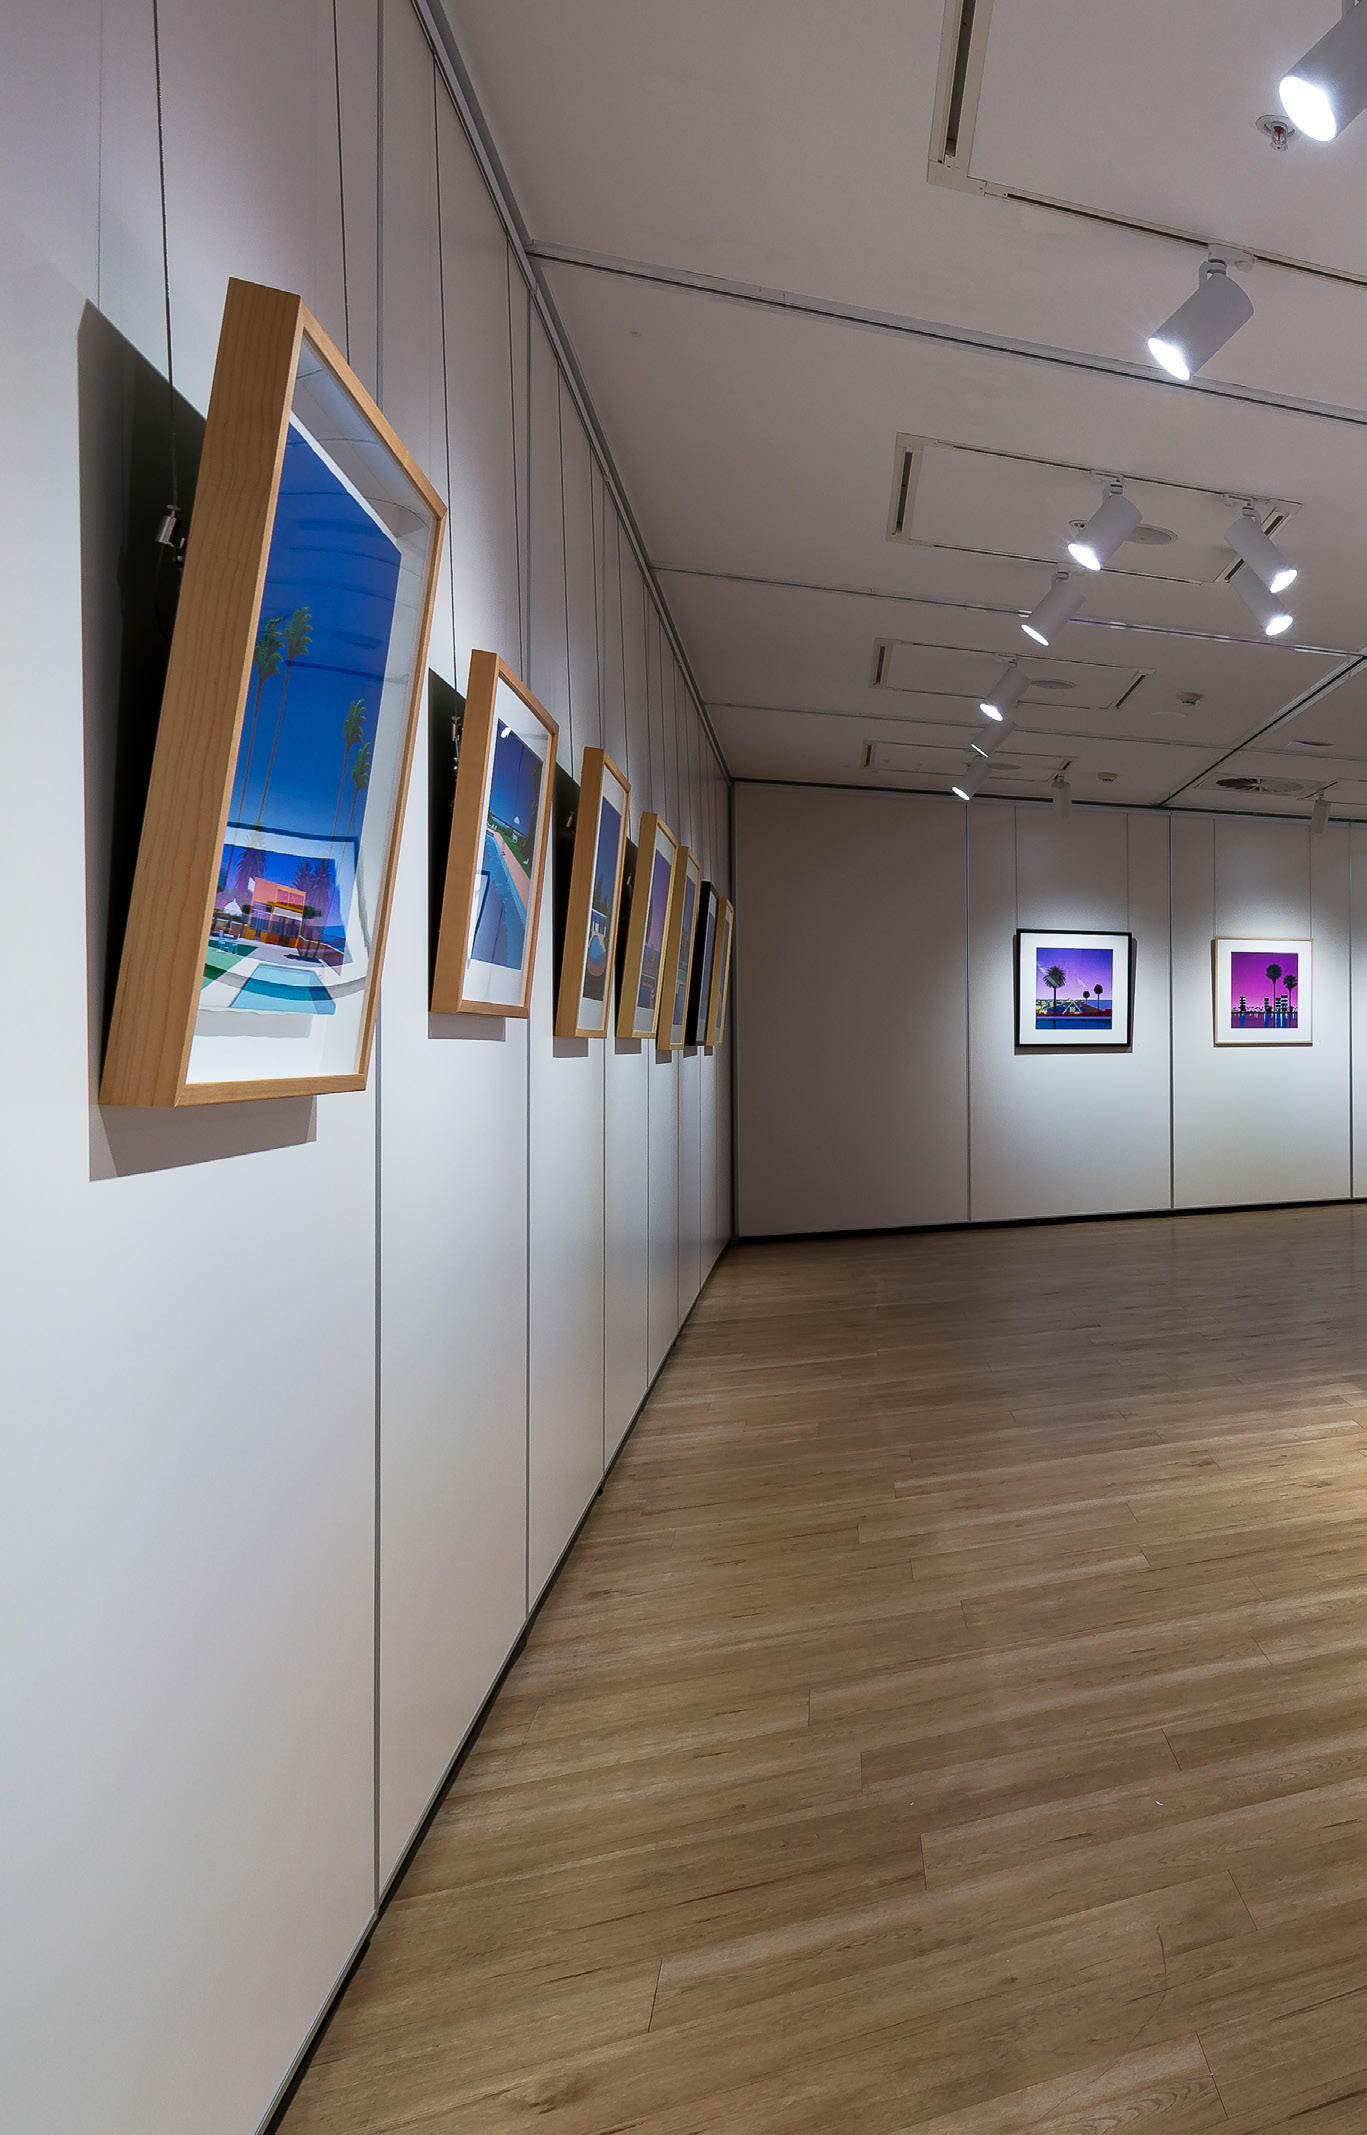
\includegraphics[width=0.52083in,height=\textheight,keepaspectratio]{img/jpf/19.jpg}
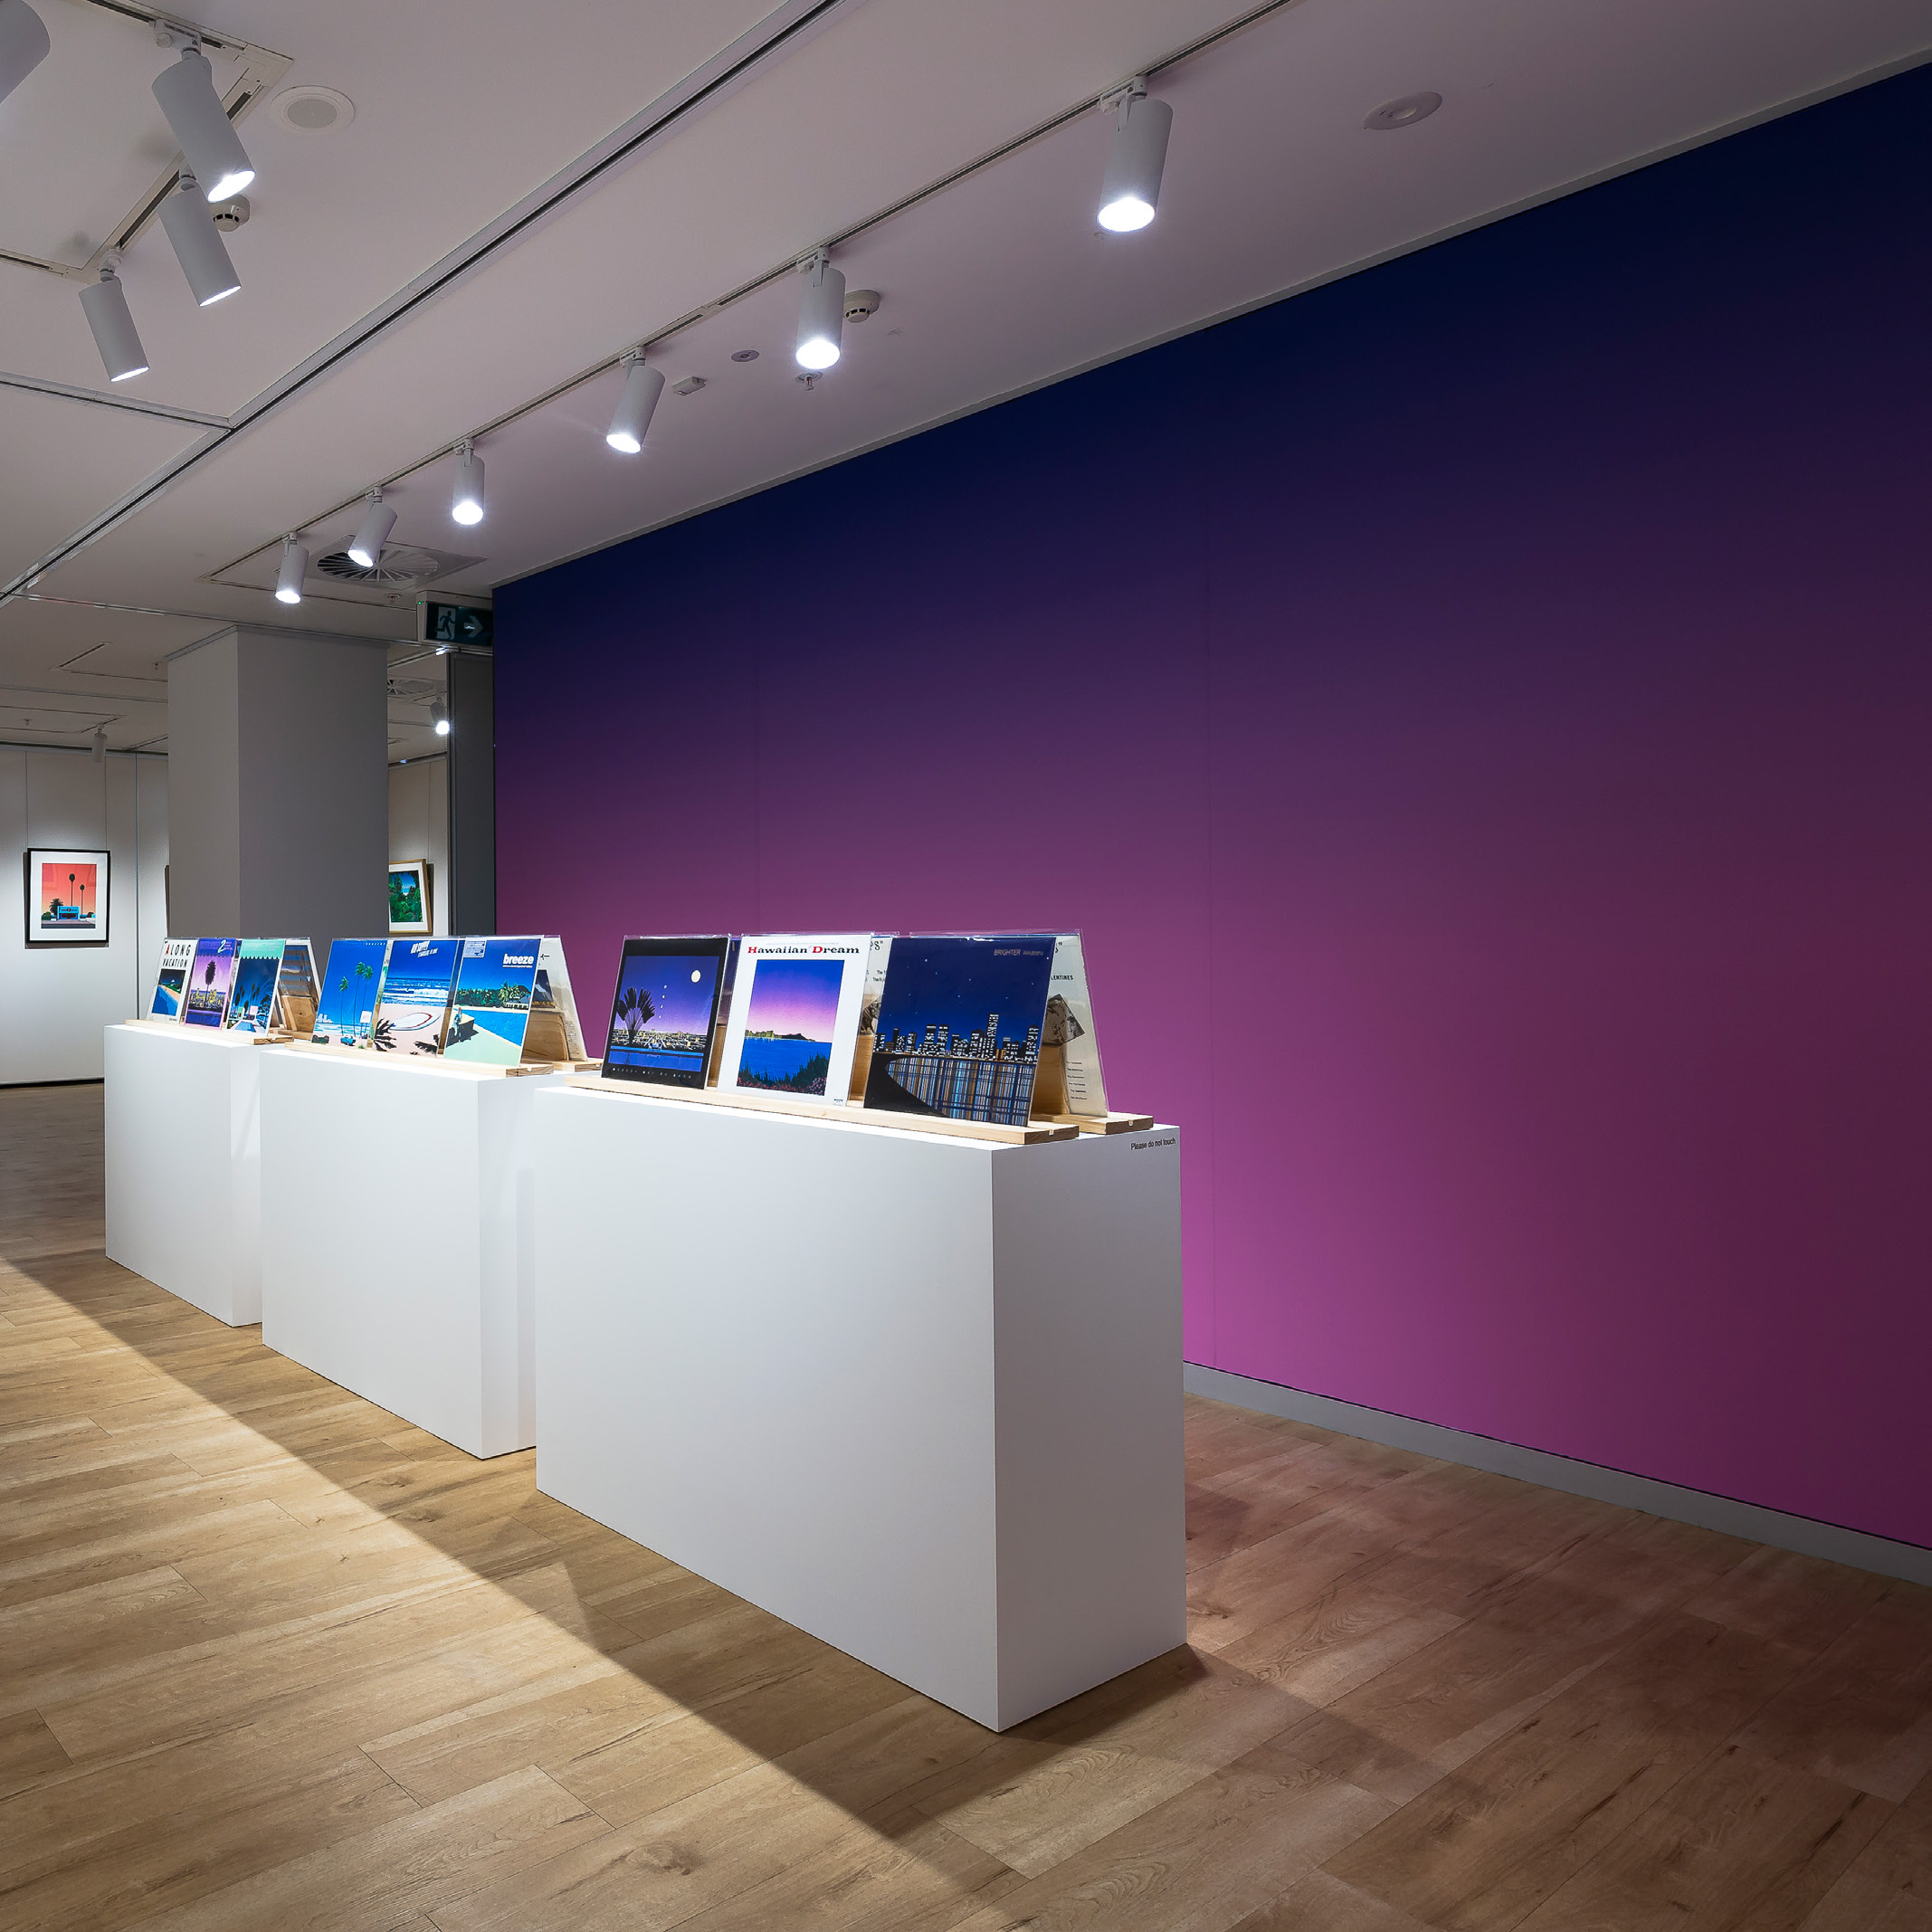
\includegraphics[width=0.52083in,height=\textheight,keepaspectratio]{img/jpf/20.jpg}

\marginnote{\begin{footnotesize}

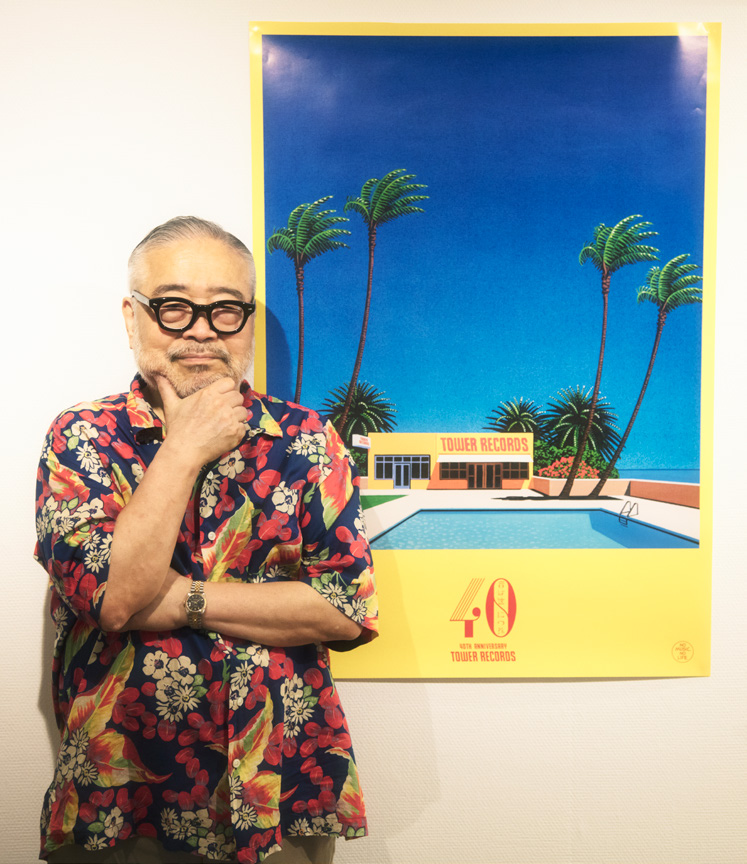
\includegraphics[width=0.52083in,height=\textheight,keepaspectratio]{img/jpf/1.jpg}
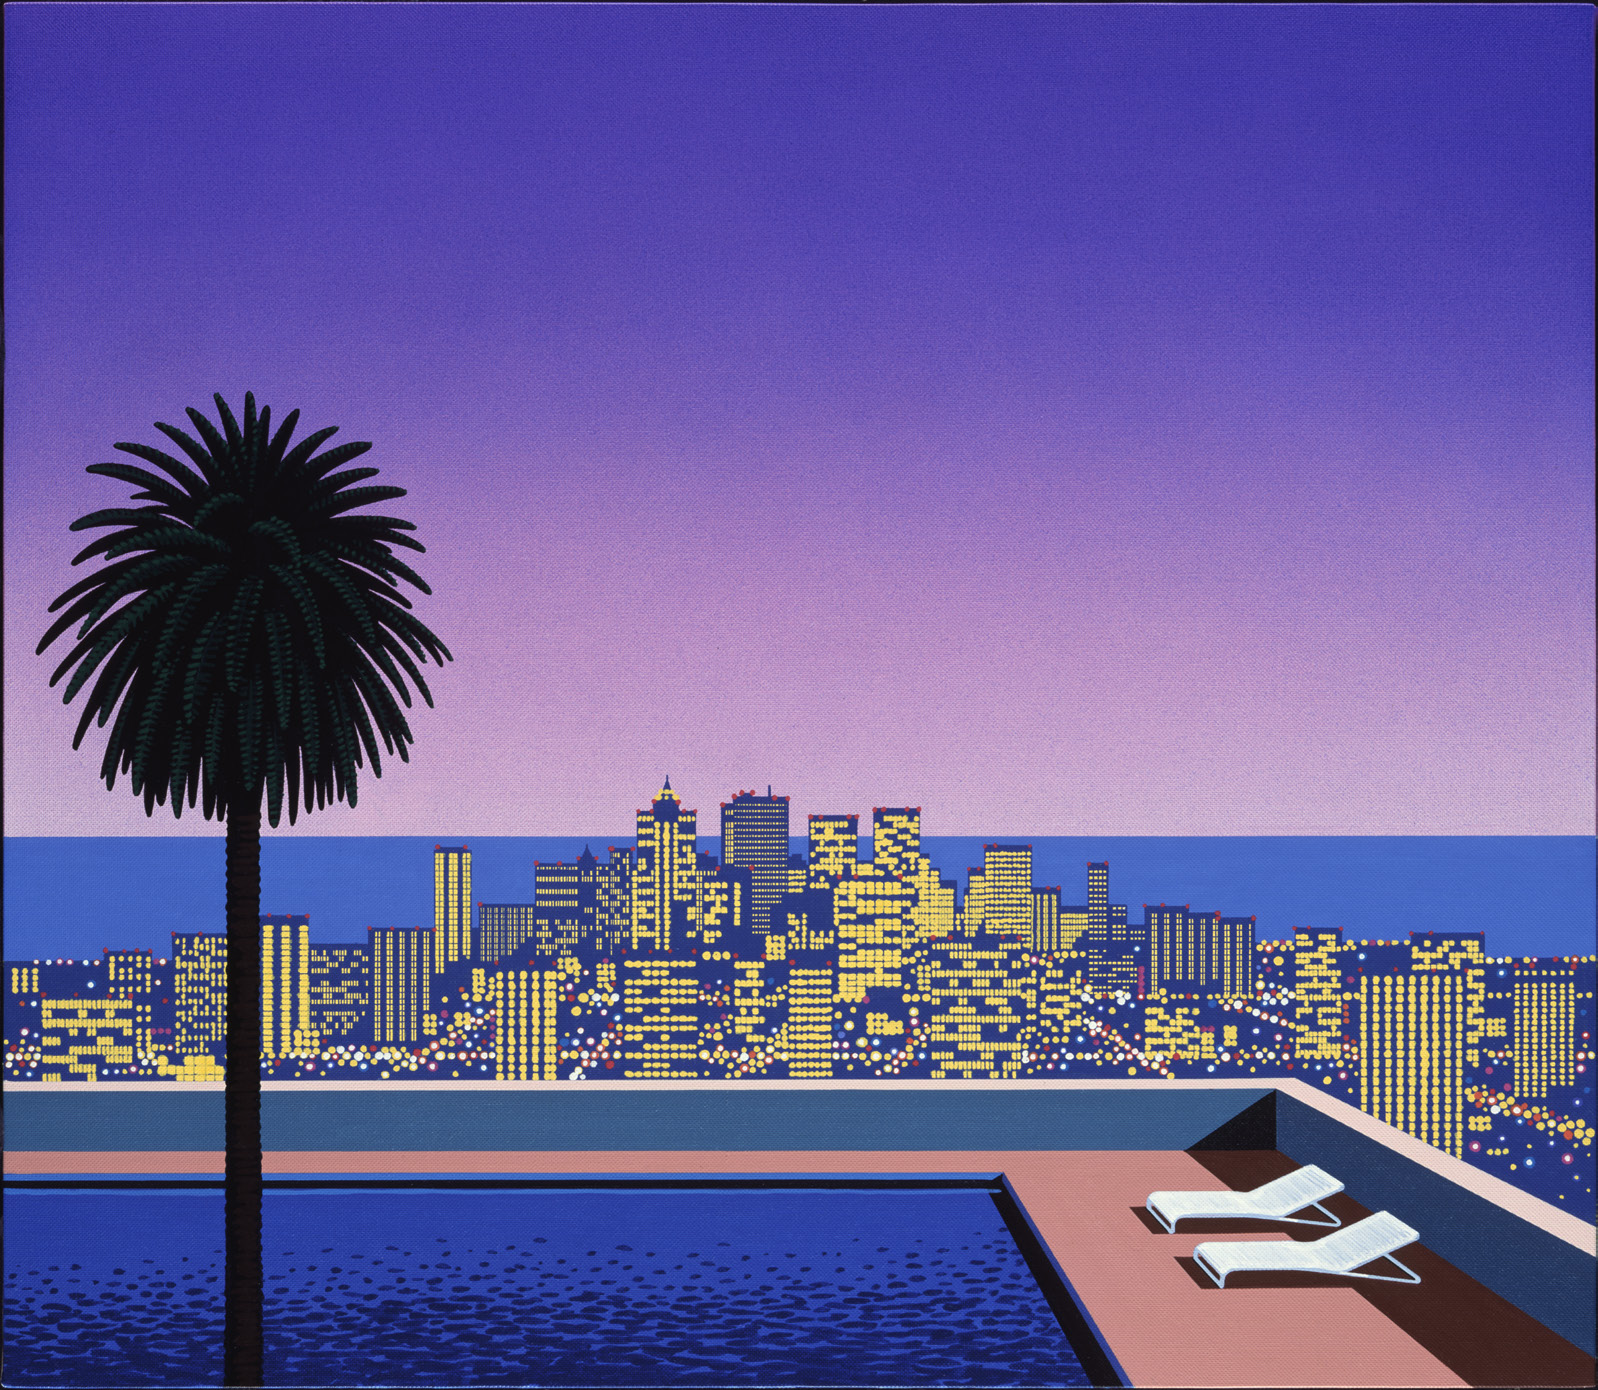
\includegraphics[width=0.52083in,height=\textheight,keepaspectratio]{img/jpf/0.jpg}
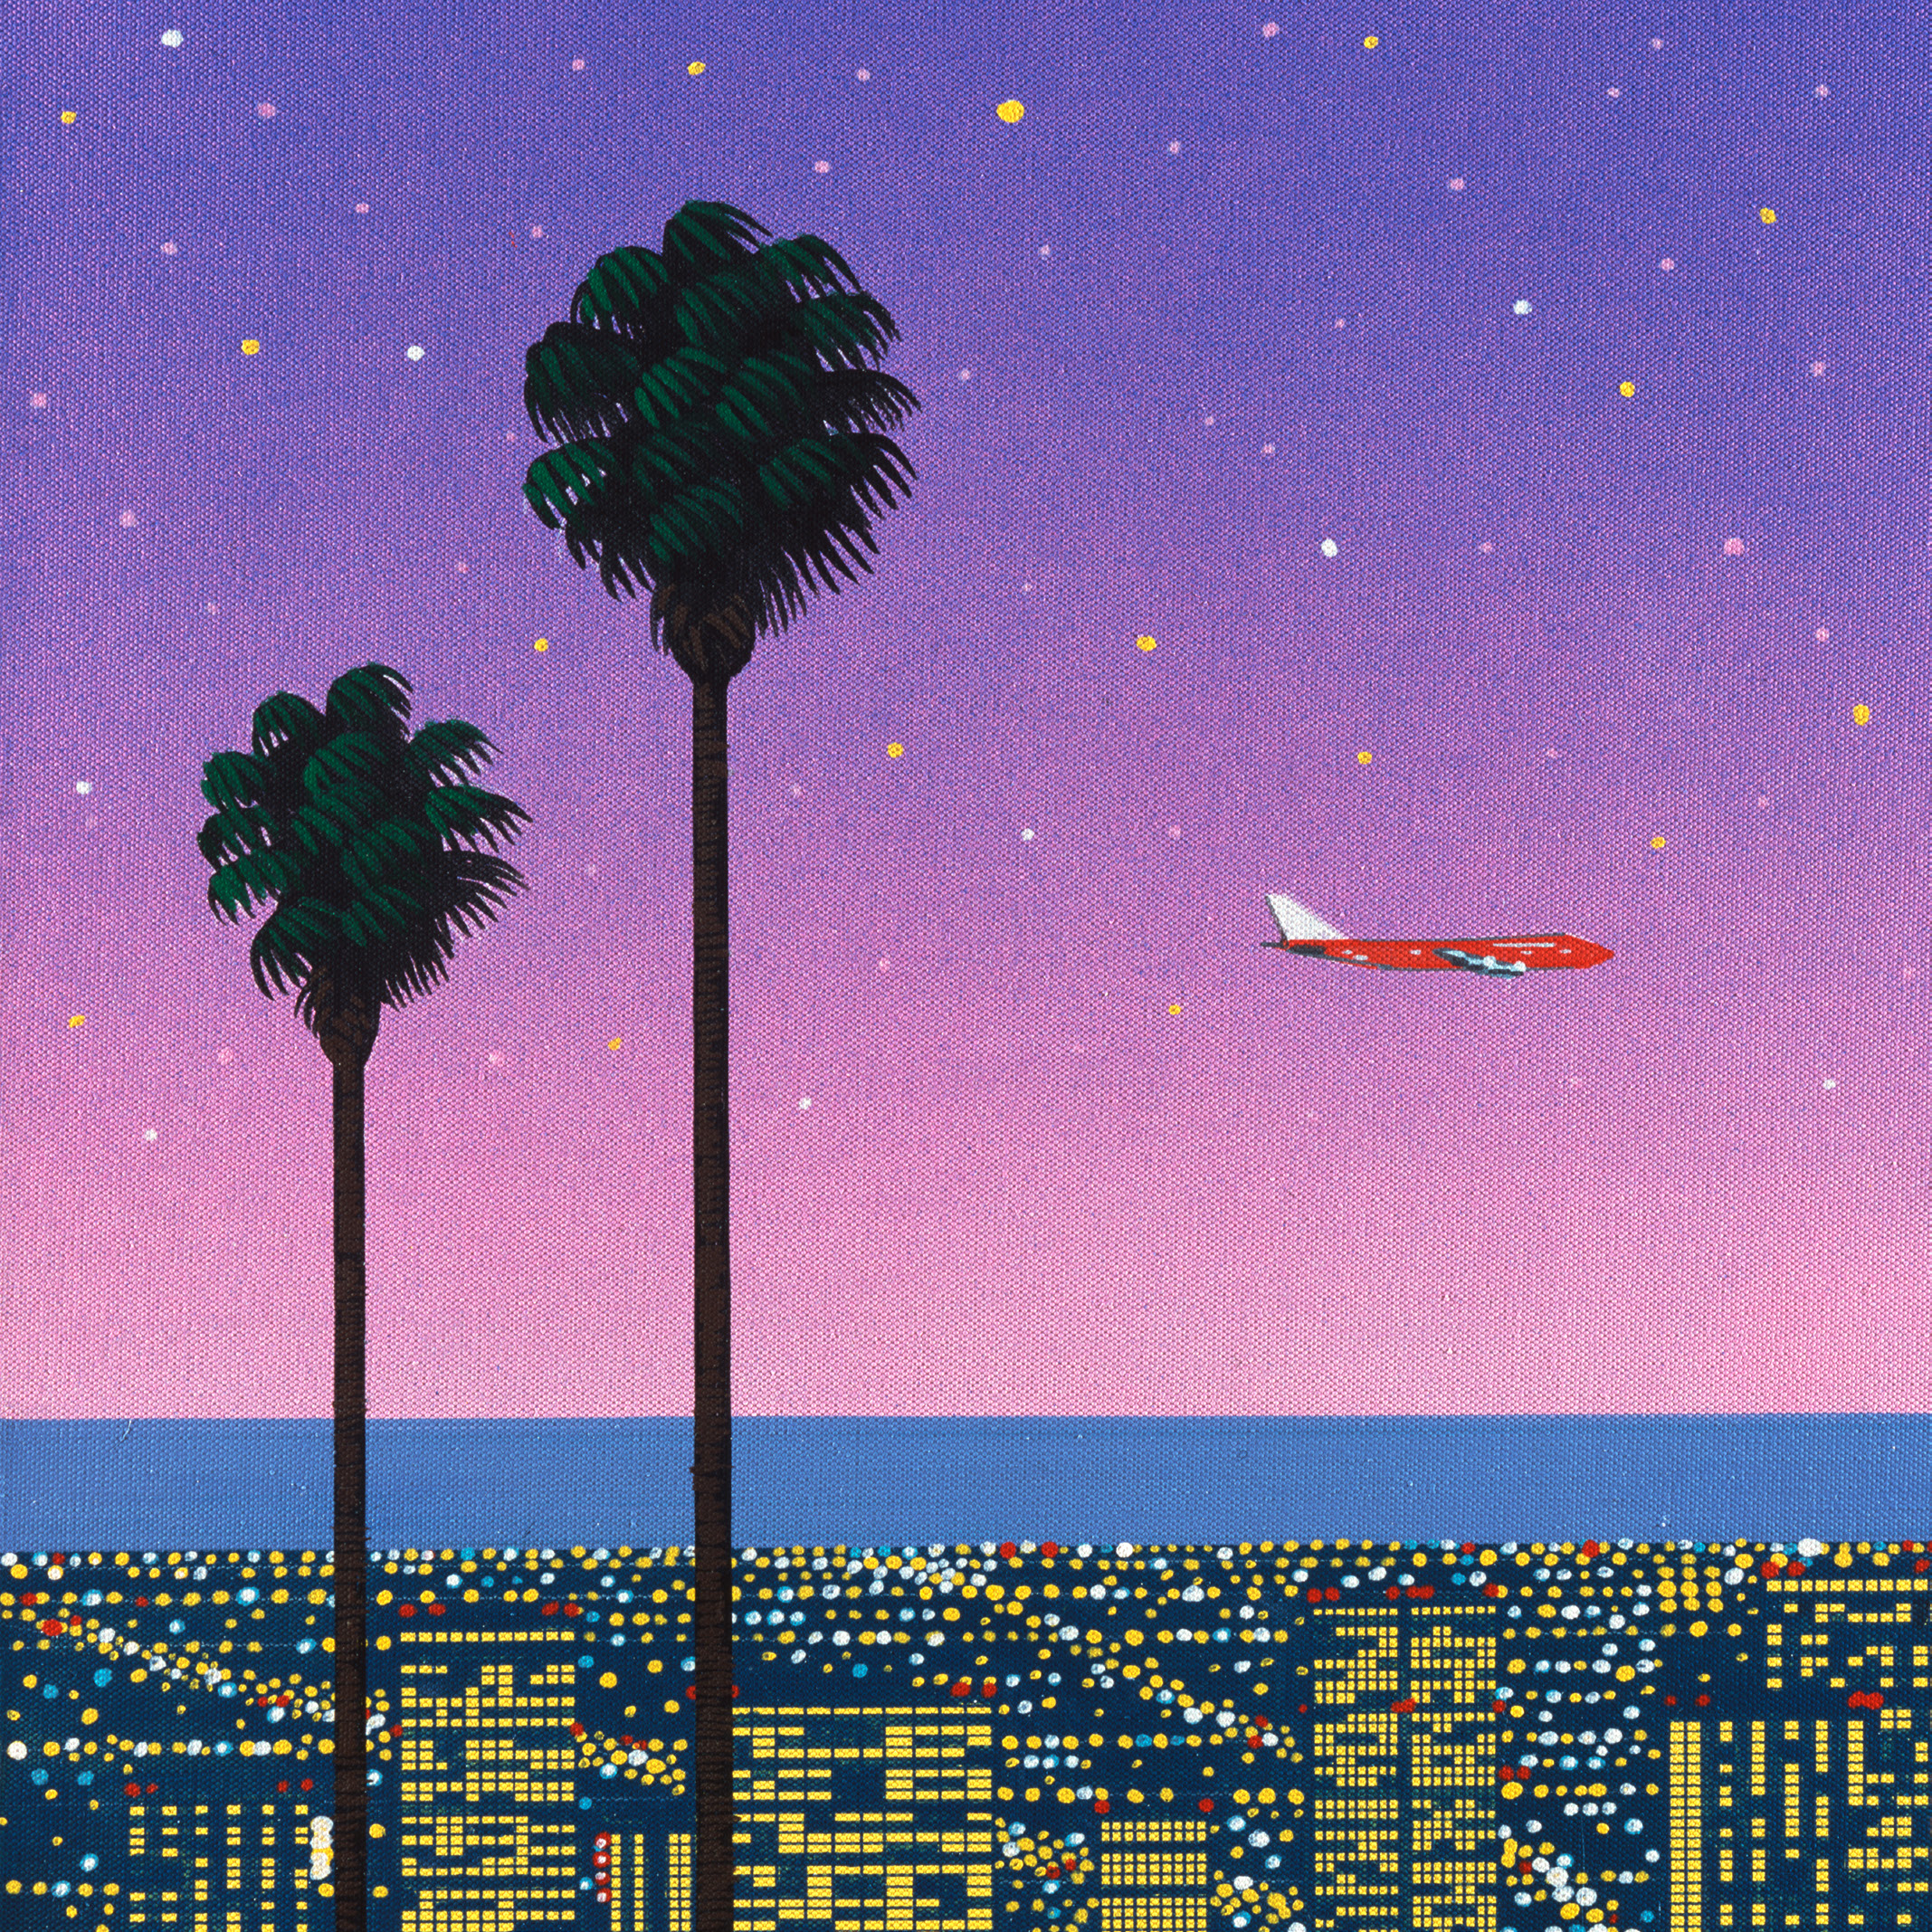
\includegraphics[width=0.52083in,height=\textheight,keepaspectratio]{img/jpf/2.jpg}
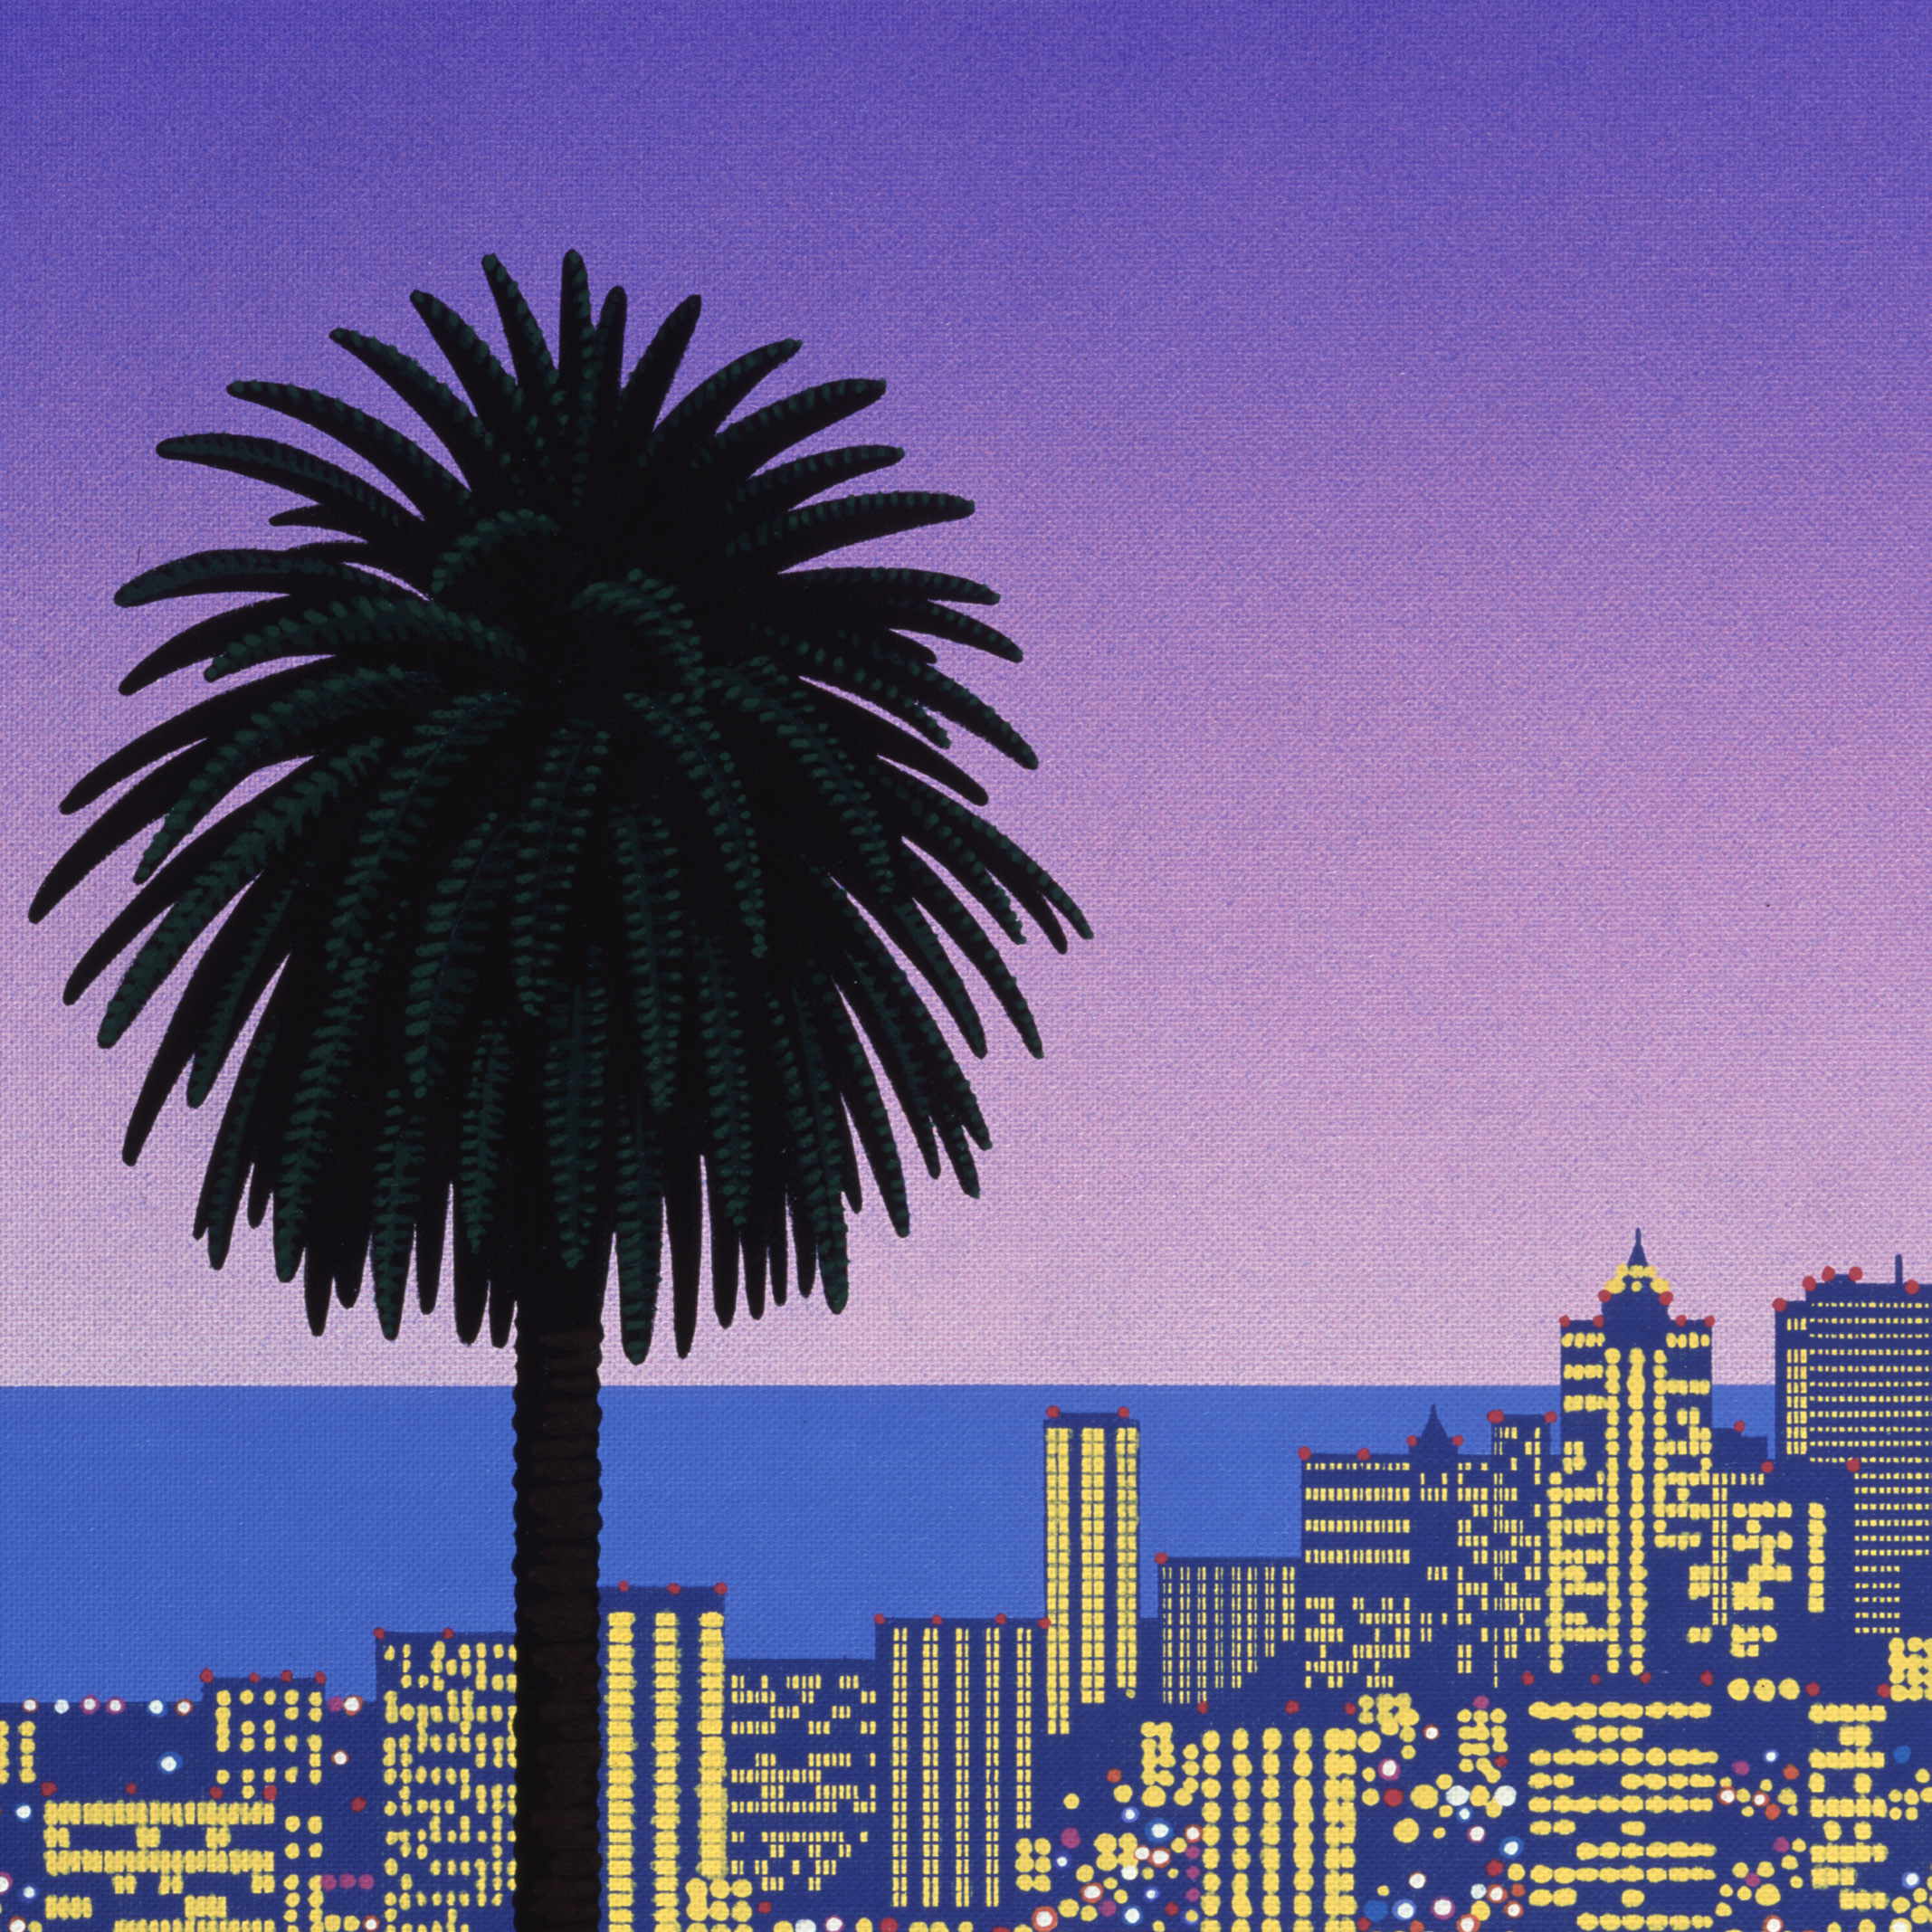
\includegraphics[width=0.52083in,height=\textheight,keepaspectratio]{img/jpf/4.jpg}
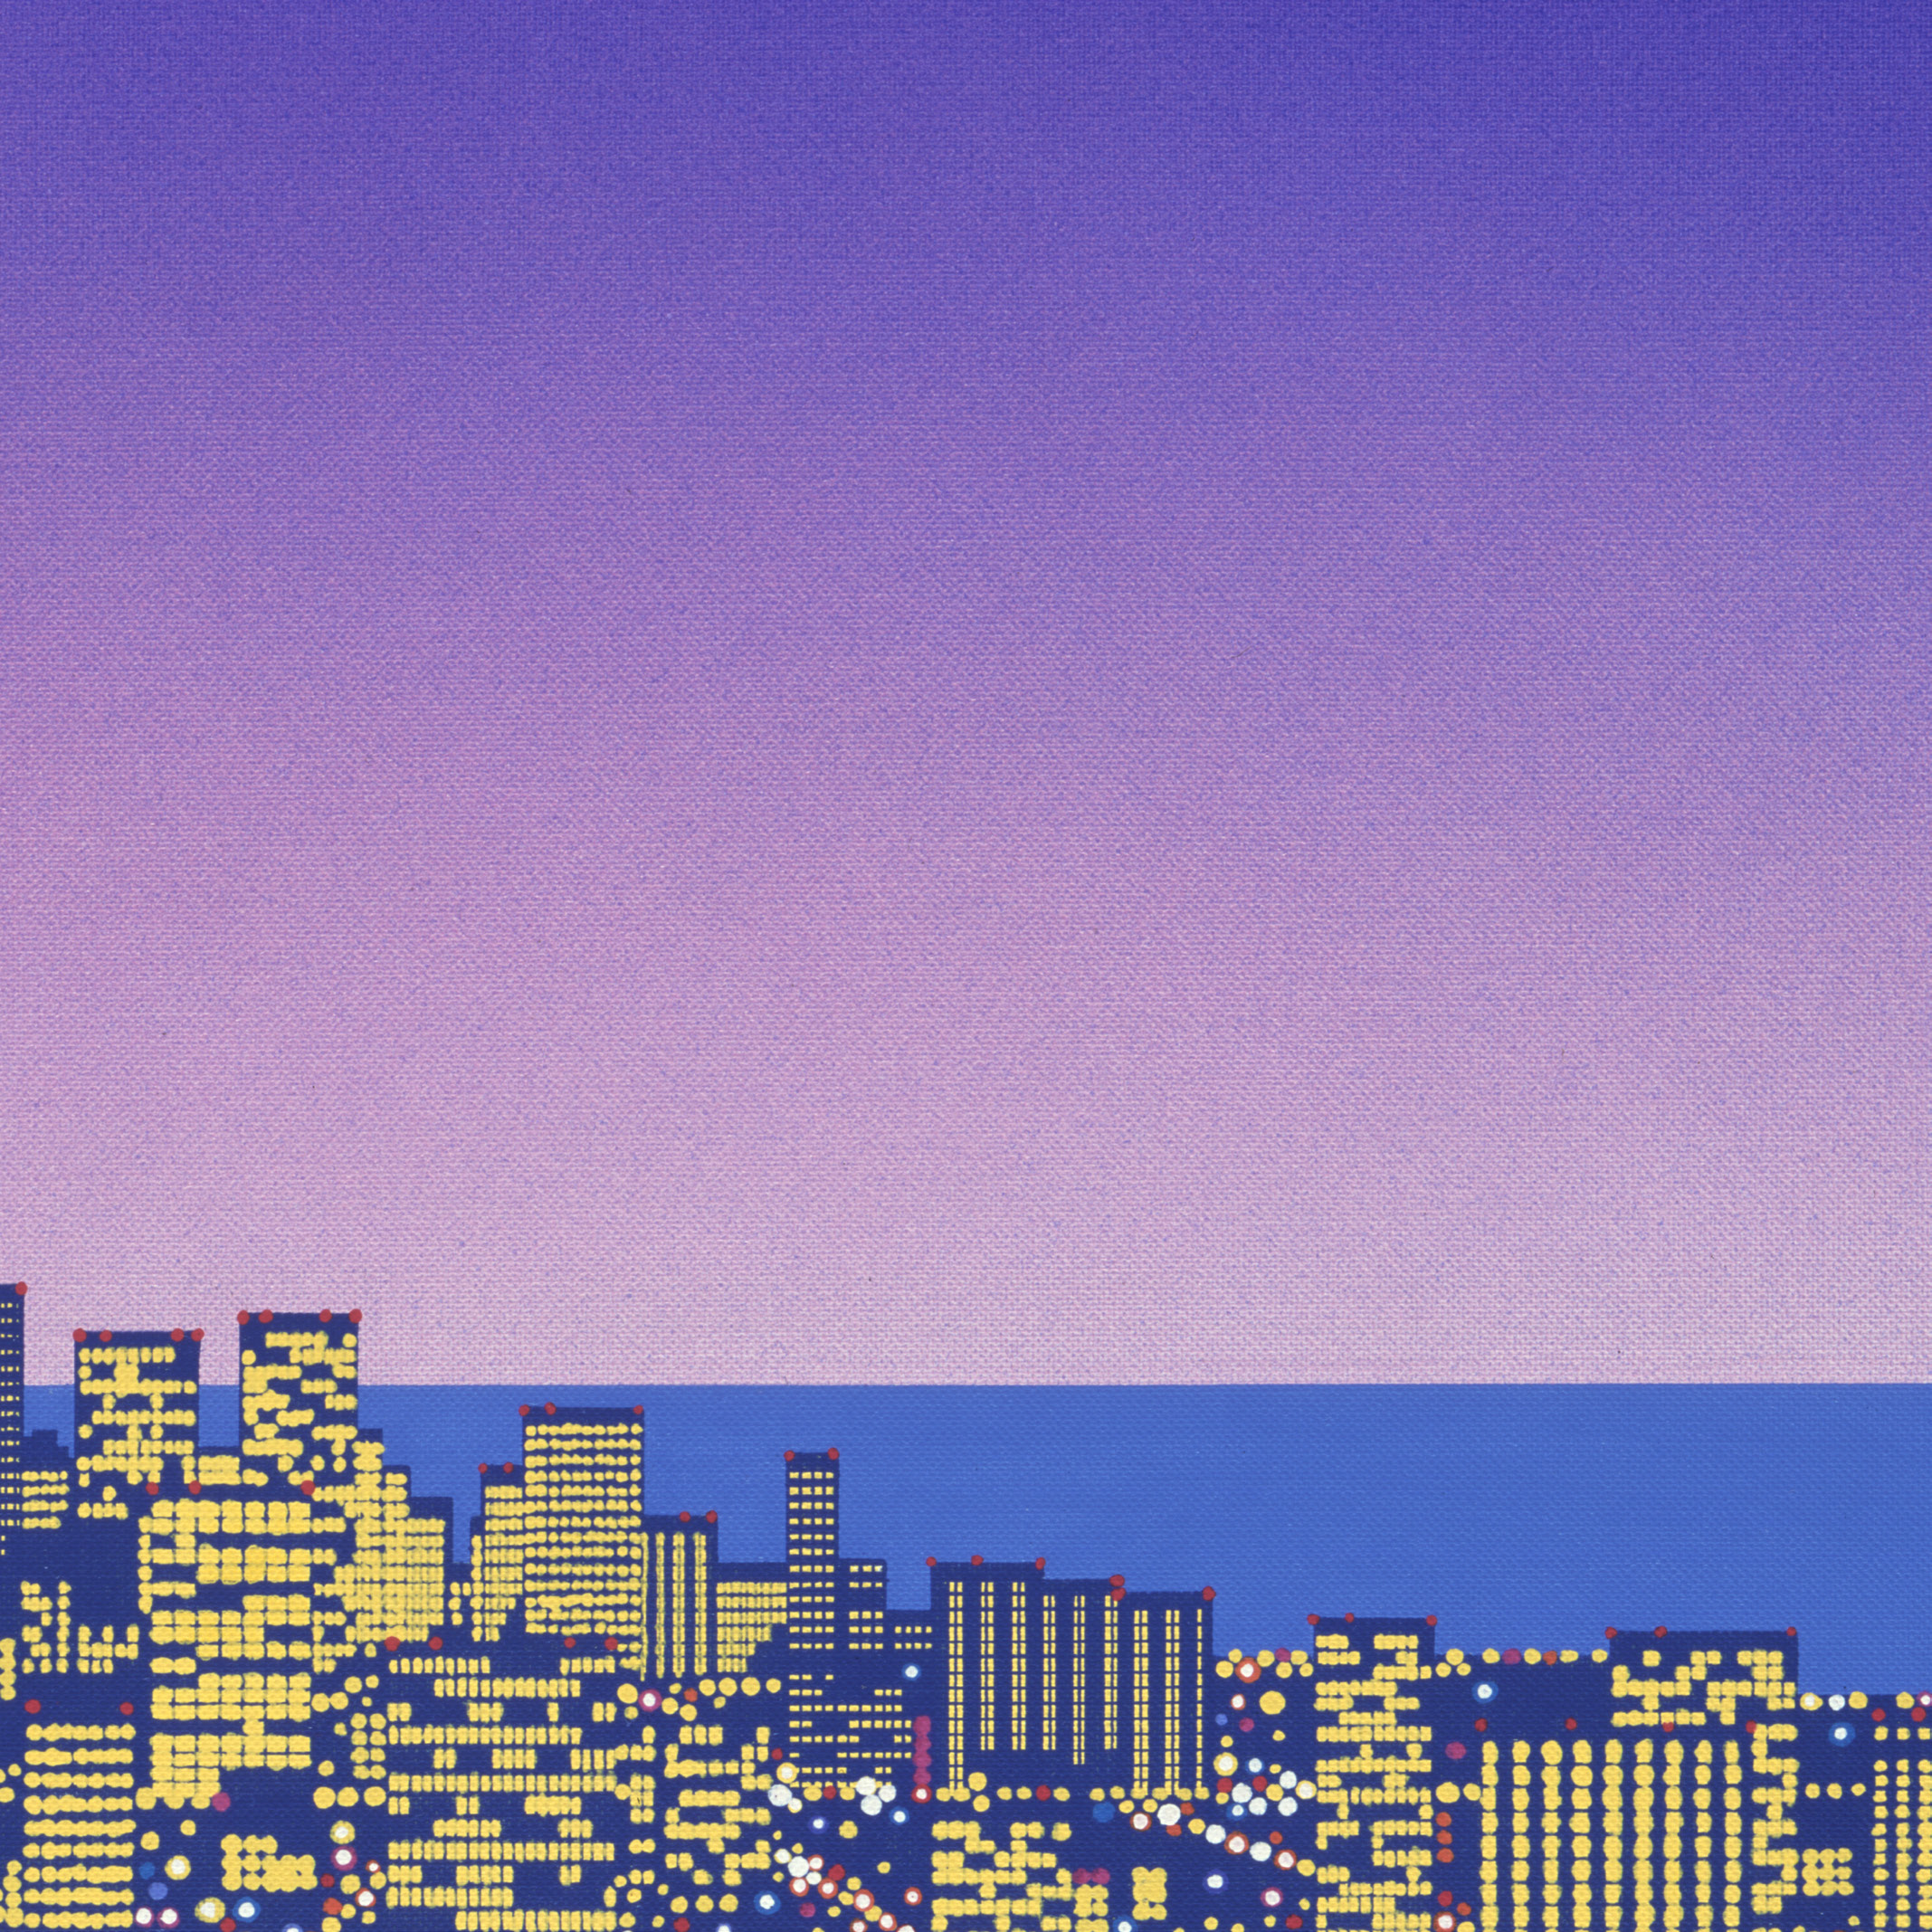
\includegraphics[width=0.52083in,height=\textheight,keepaspectratio]{img/jpf/5.jpg}
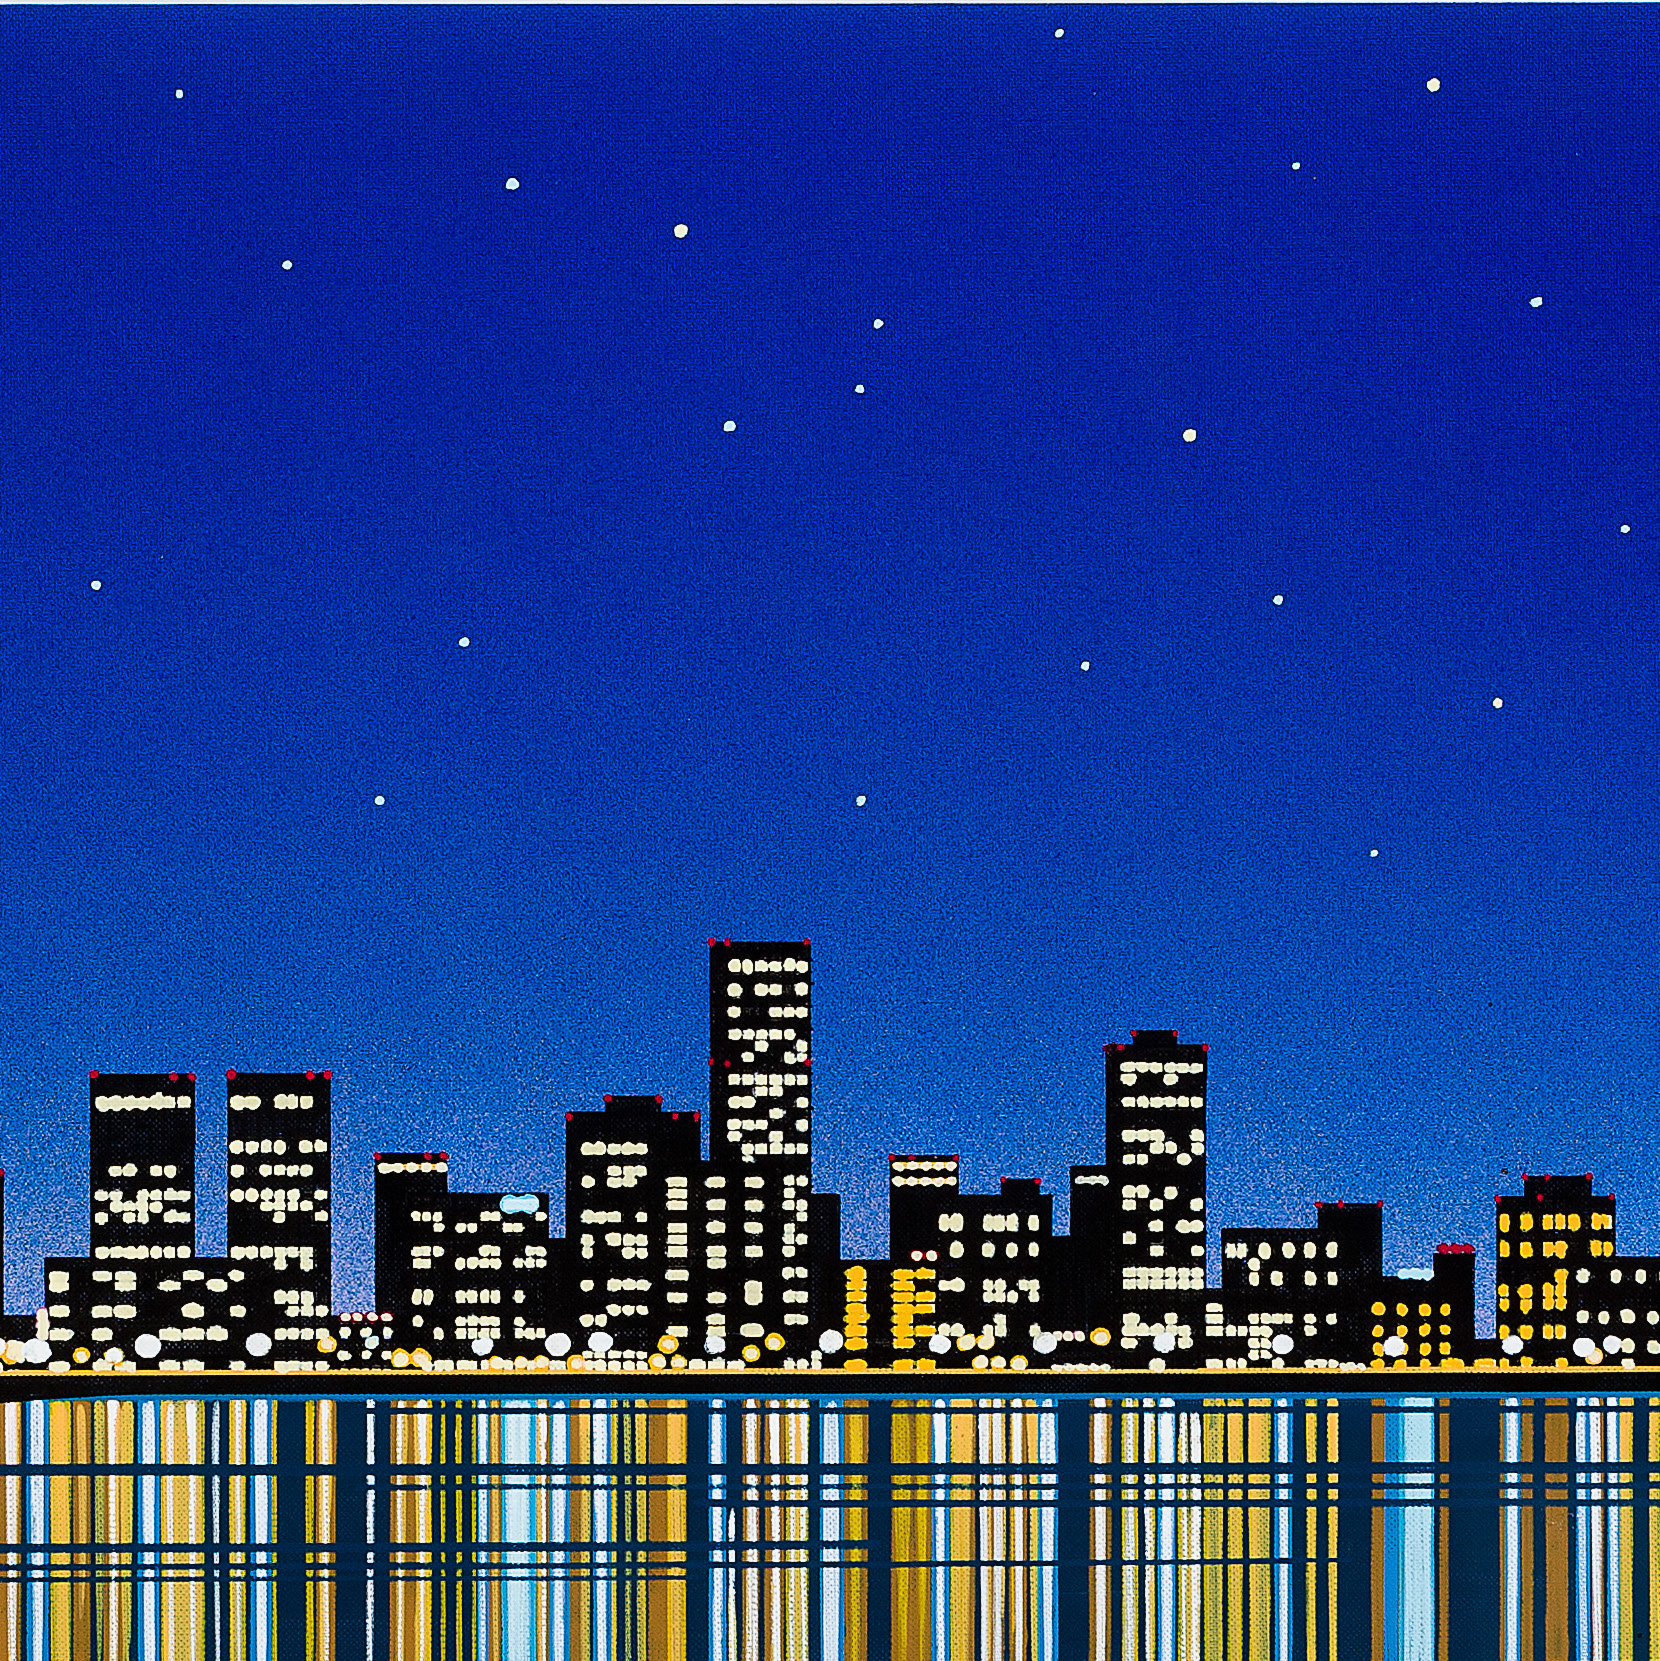
\includegraphics[width=0.52083in,height=\textheight,keepaspectratio]{img/jpf/6.jpg}
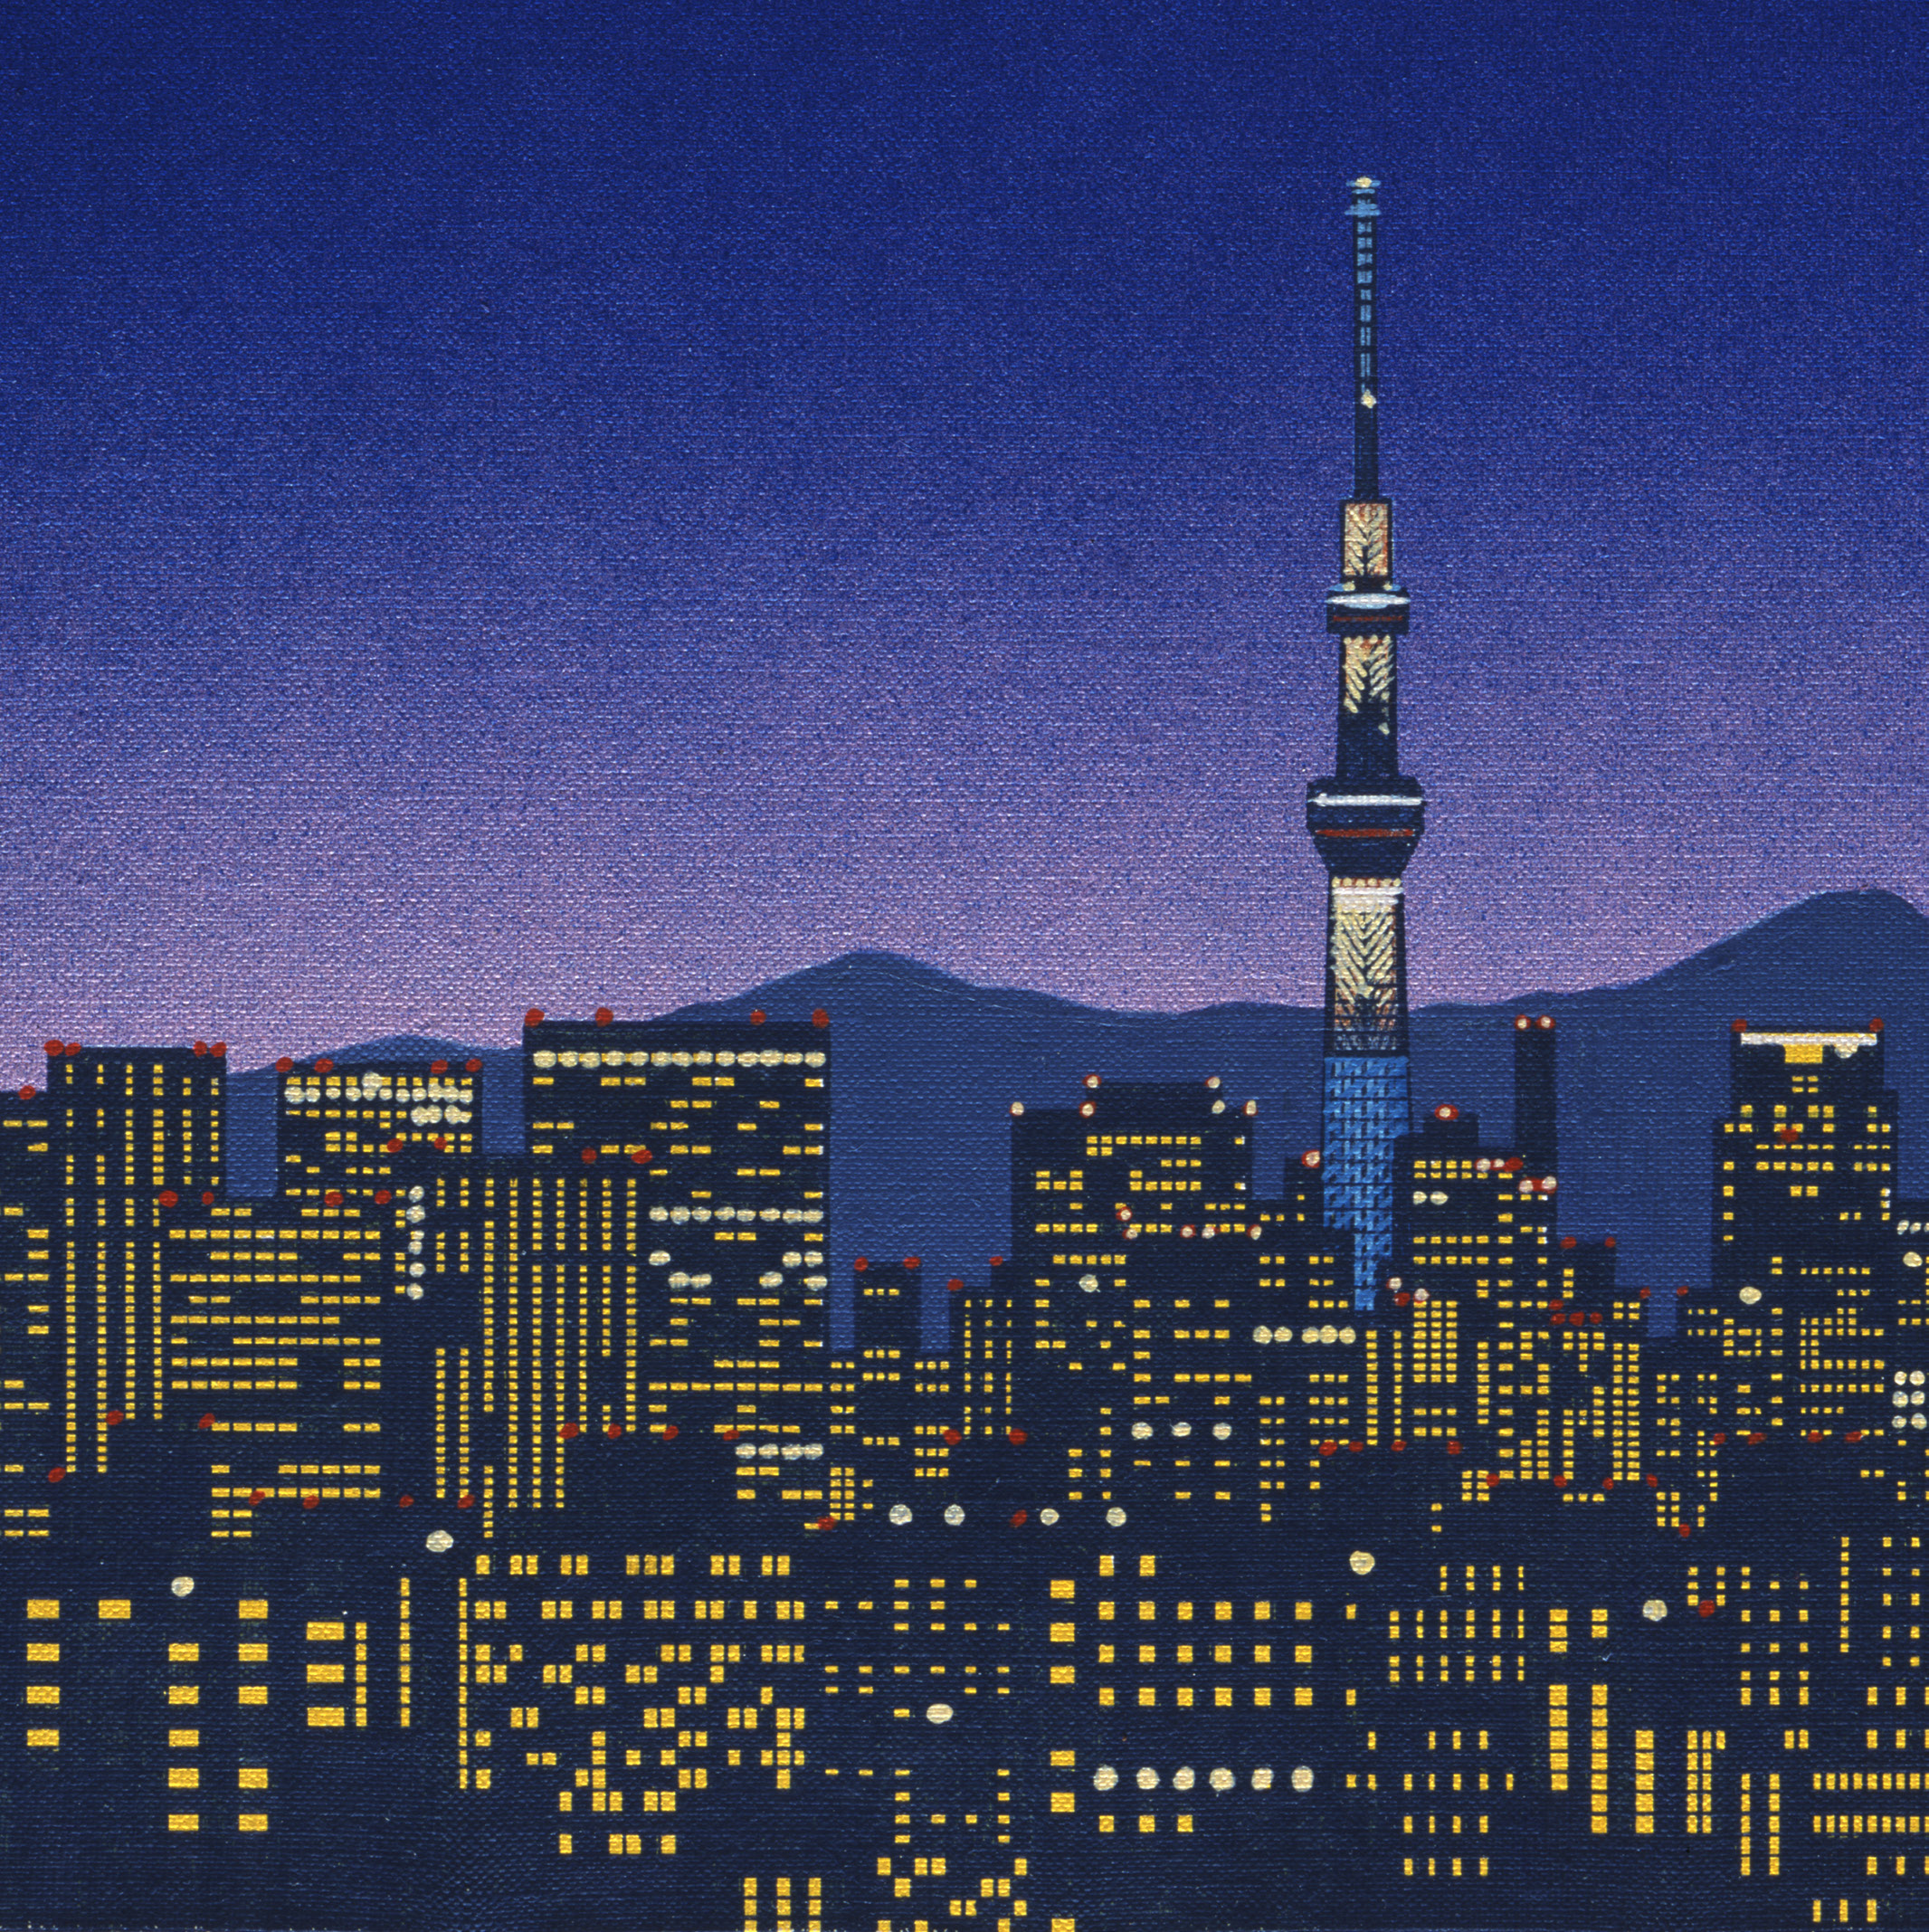
\includegraphics[width=0.52083in,height=\textheight,keepaspectratio]{img/jpf/7.jpg}
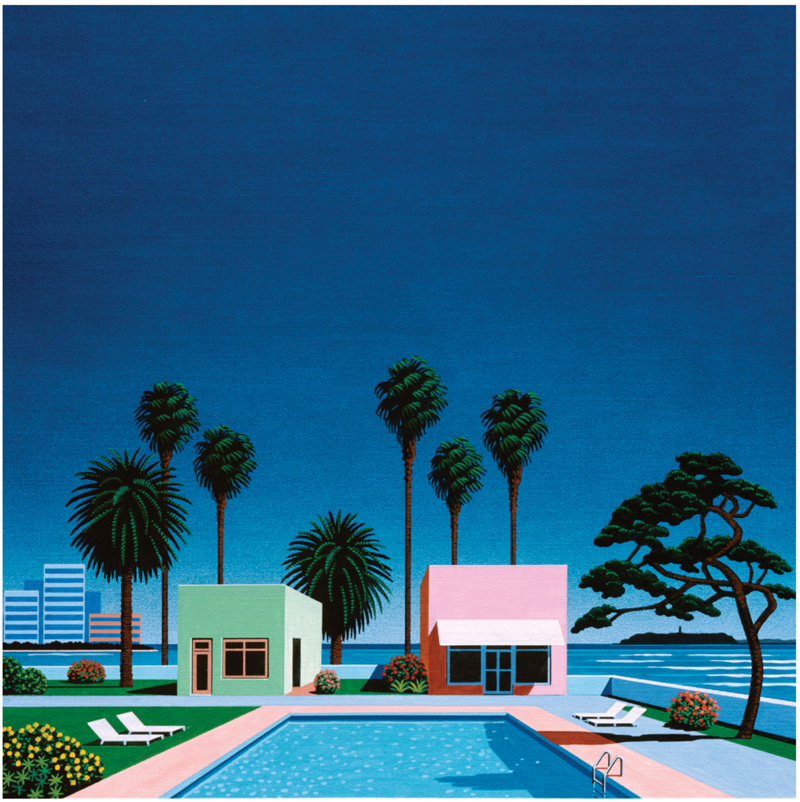
\includegraphics[width=0.52083in,height=\textheight,keepaspectratio]{img/jpf/8.jpg}

\end{footnotesize}}

\marginnote{\begin{footnotesize}

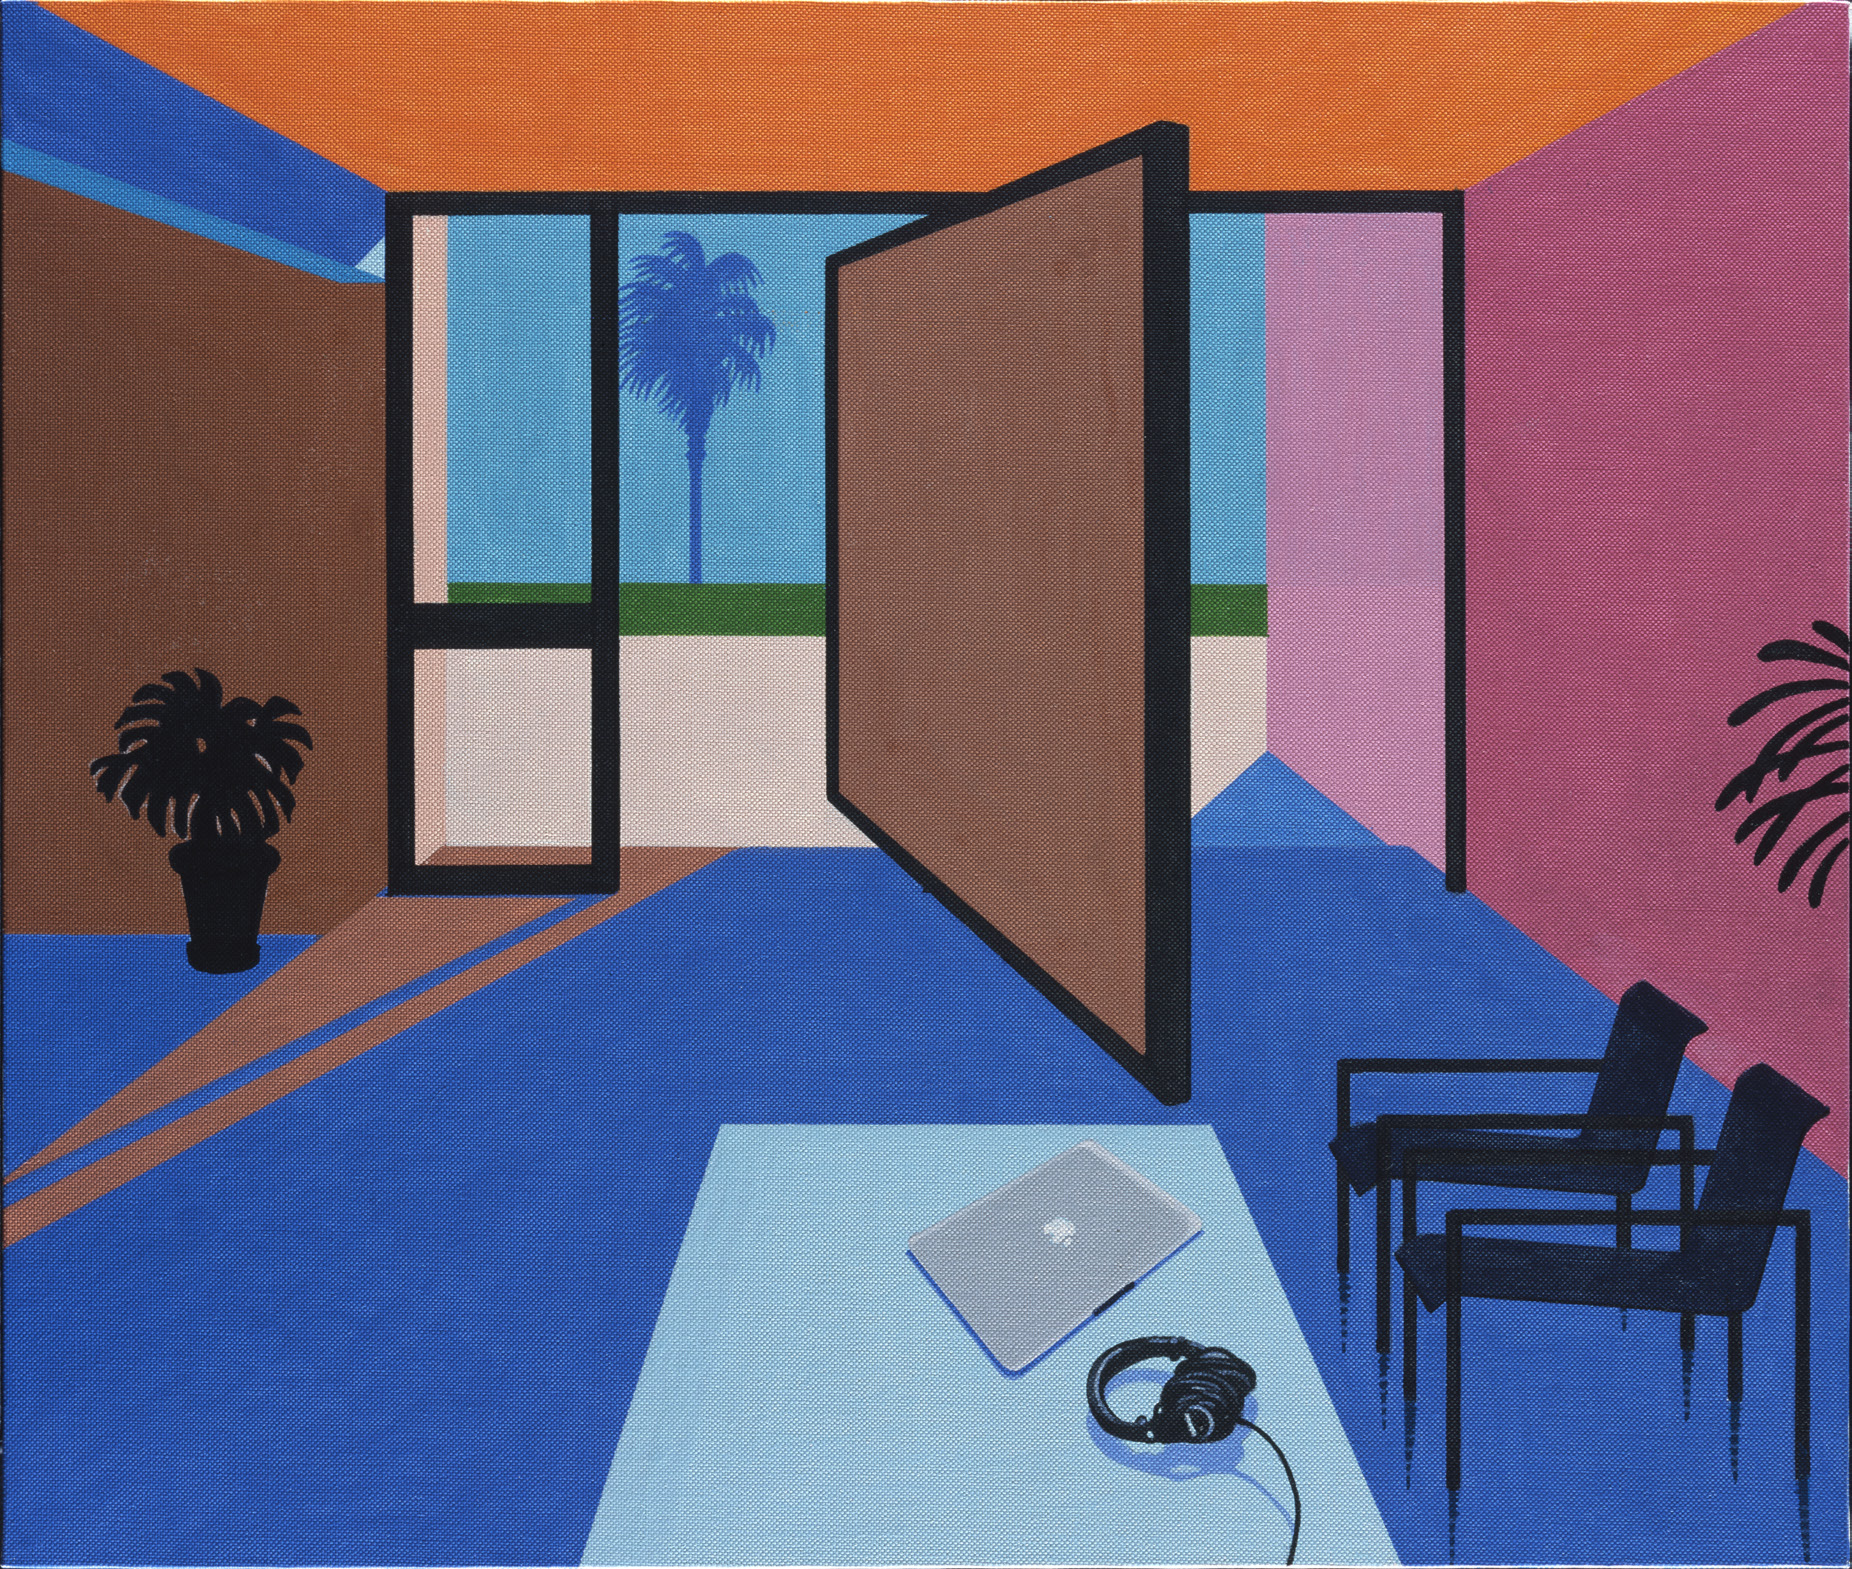
\includegraphics[width=0.52083in,height=\textheight,keepaspectratio]{img/jpf/21.jpg}
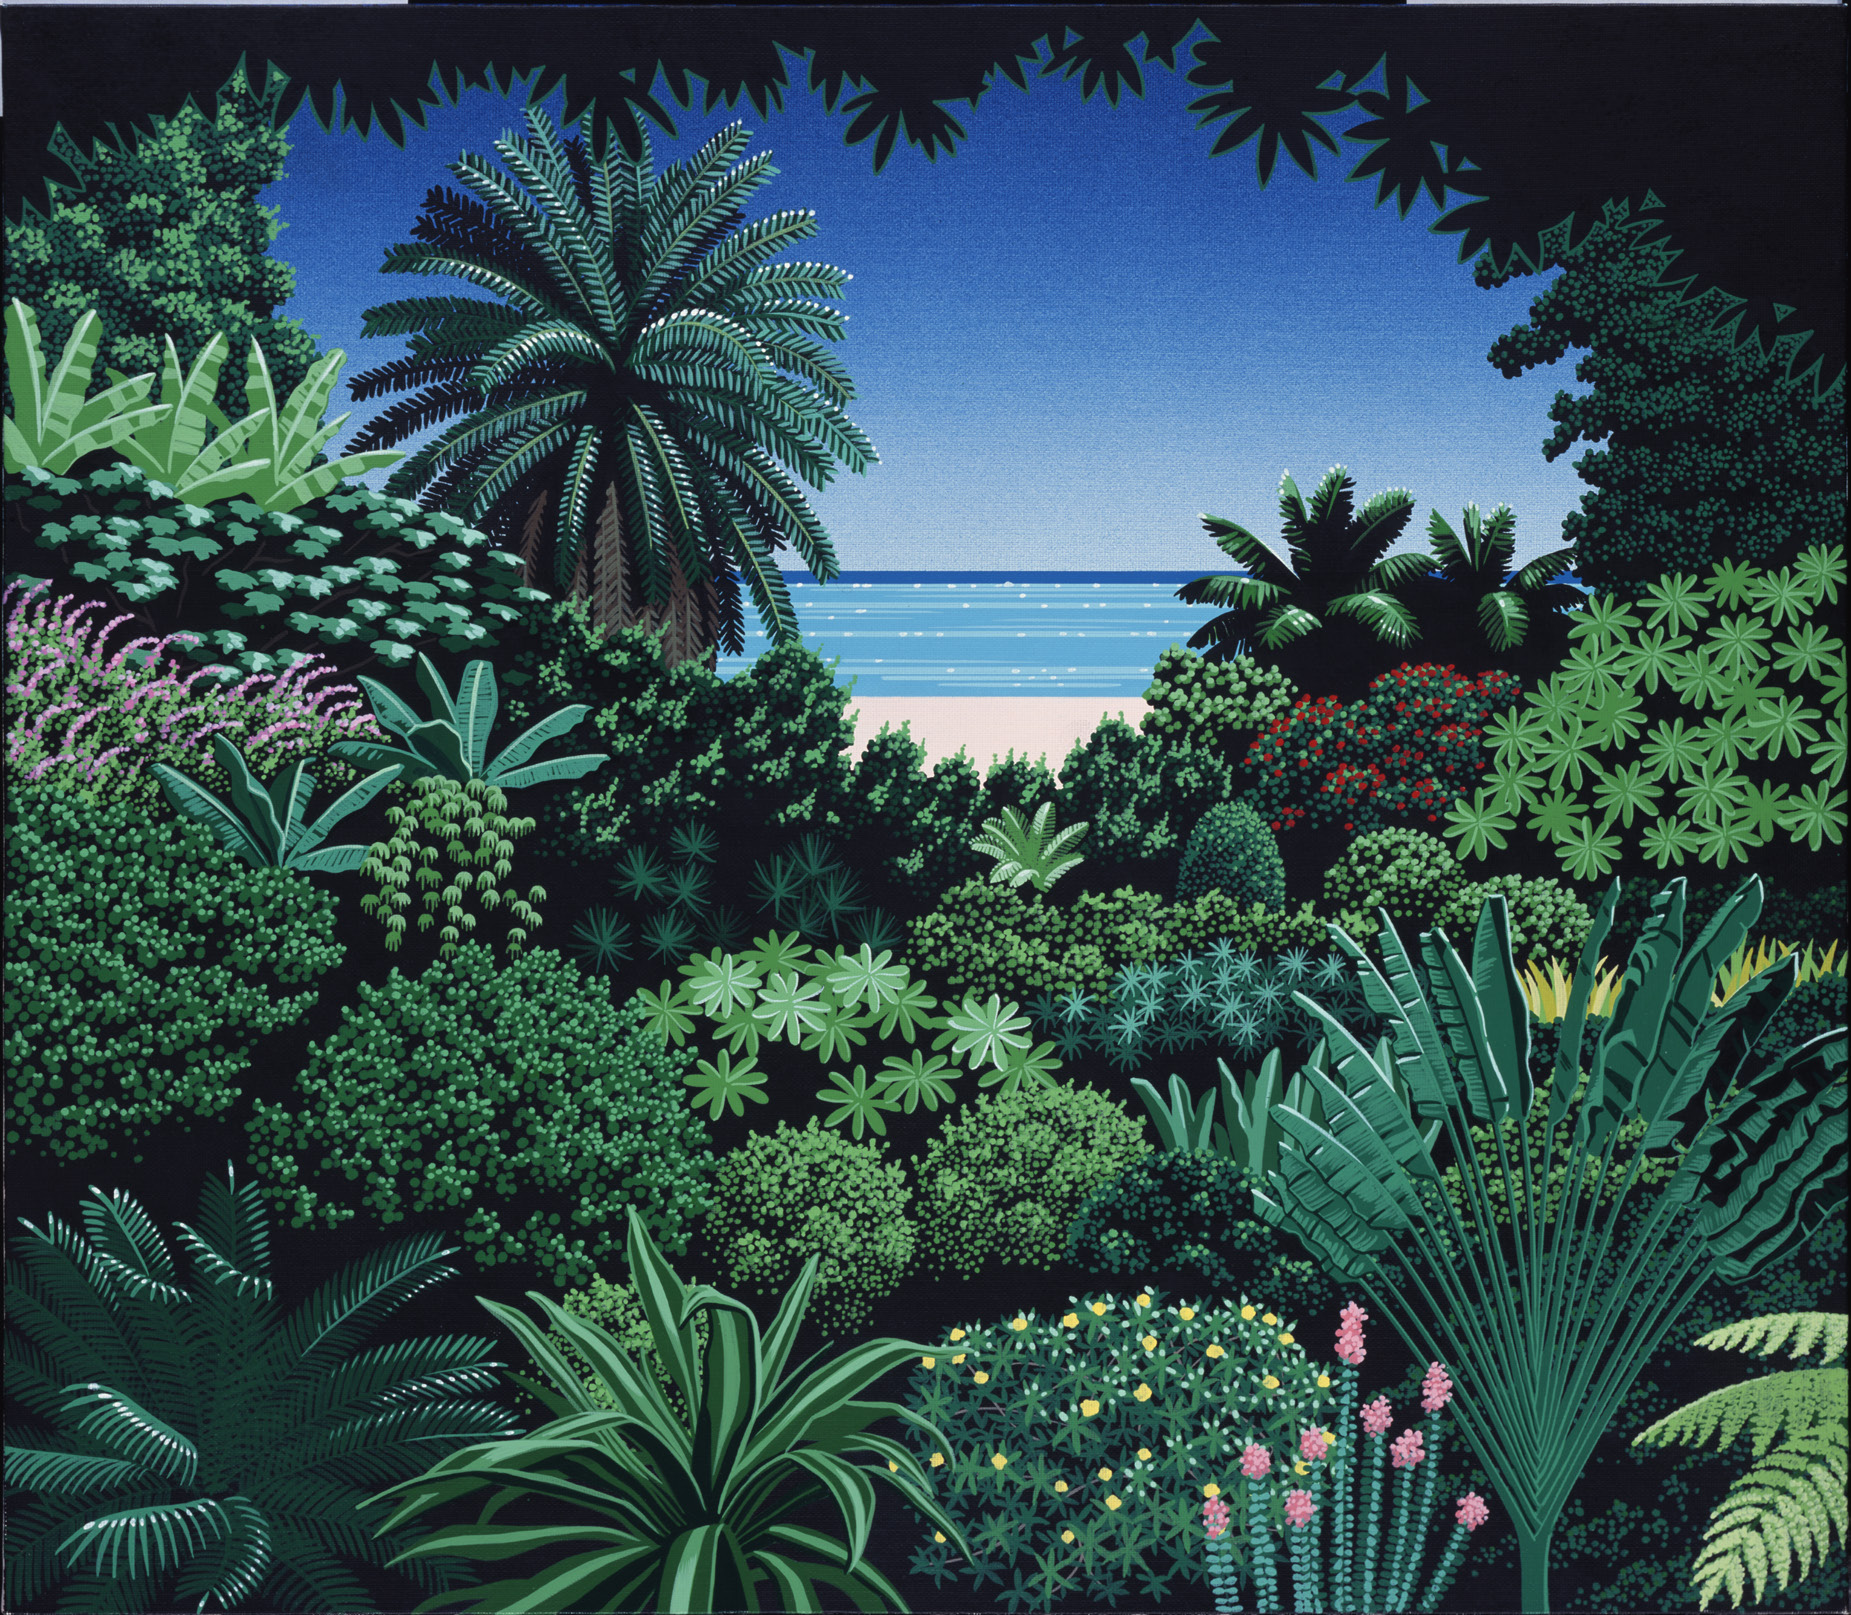
\includegraphics[width=0.52083in,height=\textheight,keepaspectratio]{img/jpf/22.jpg}
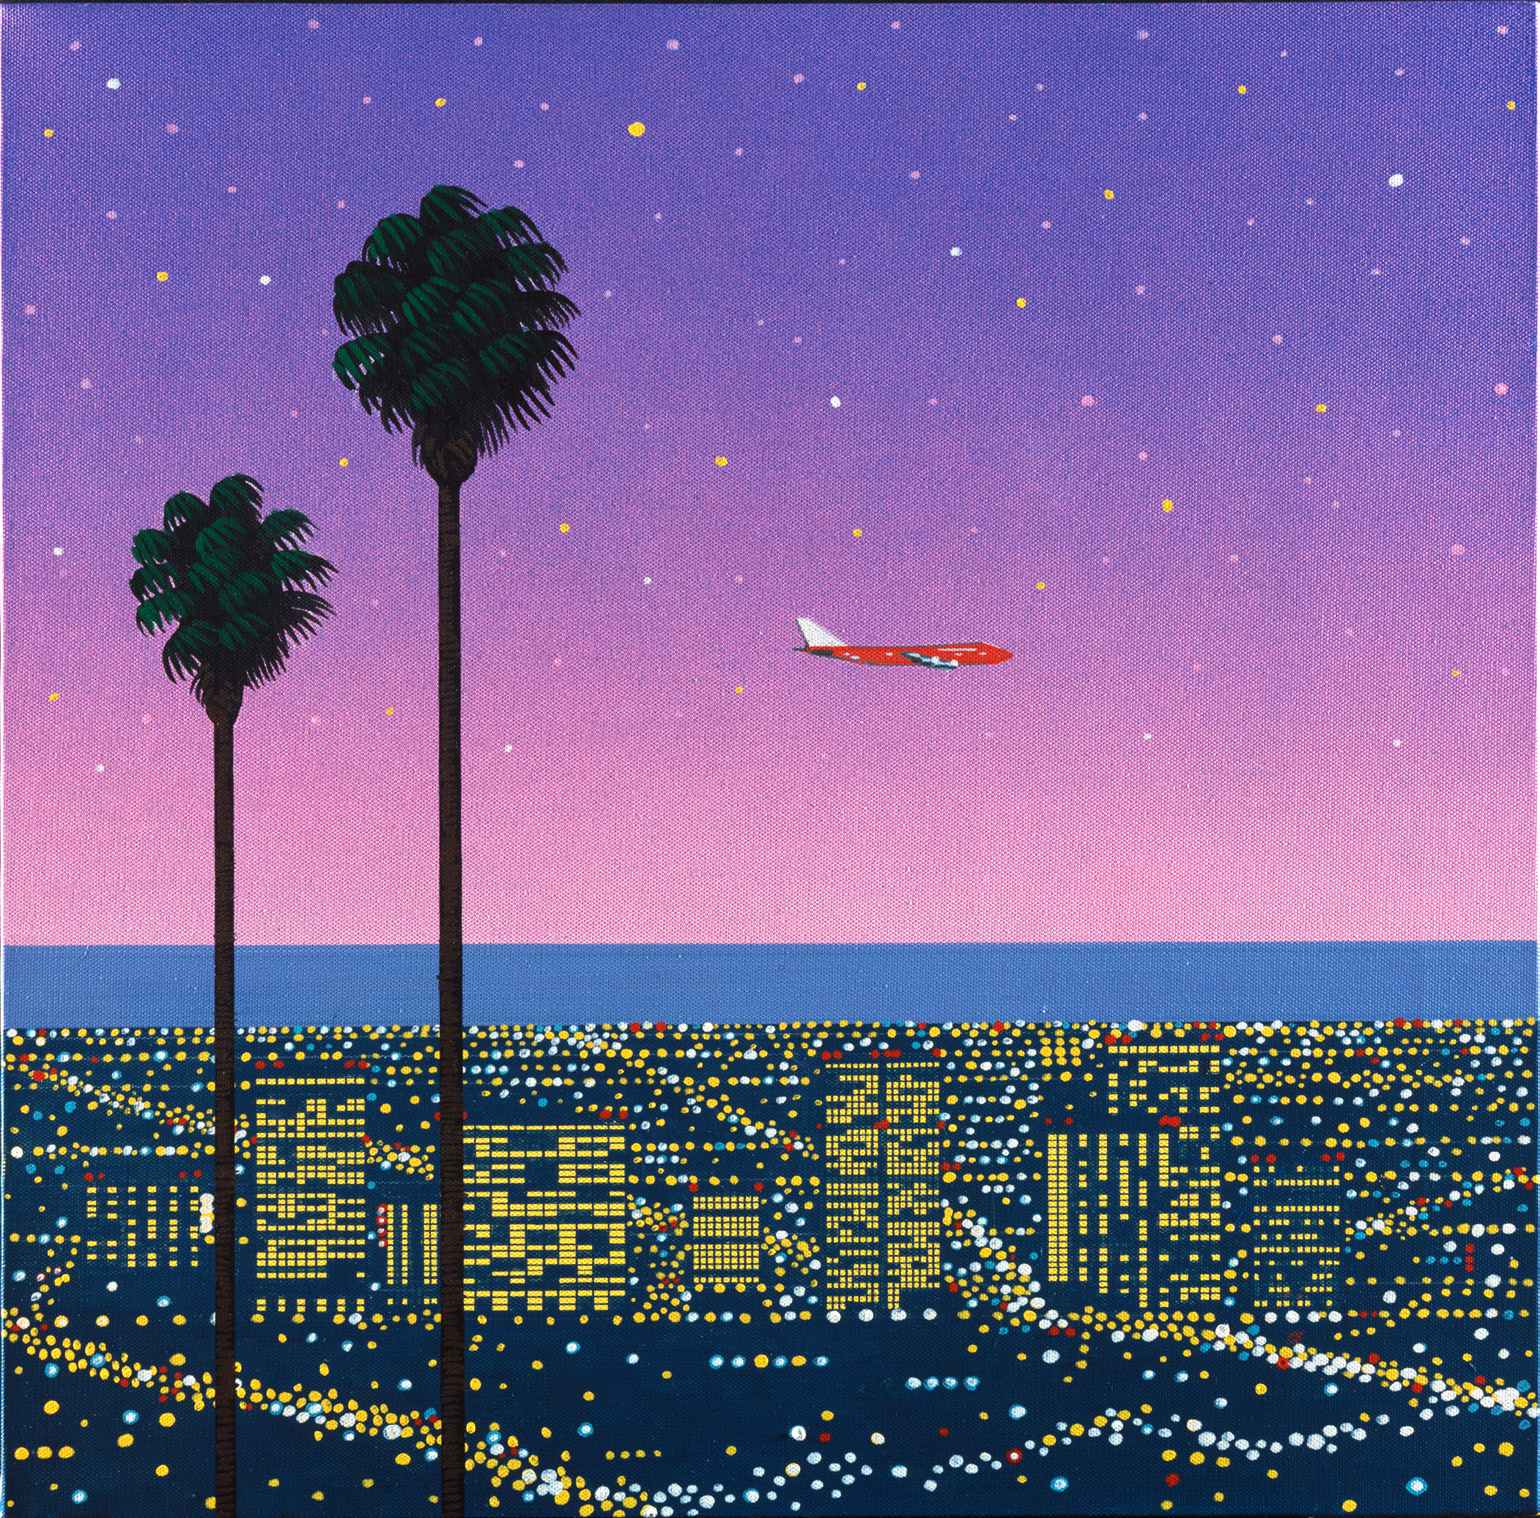
\includegraphics[width=0.52083in,height=\textheight,keepaspectratio]{img/jpf/23.jpg}
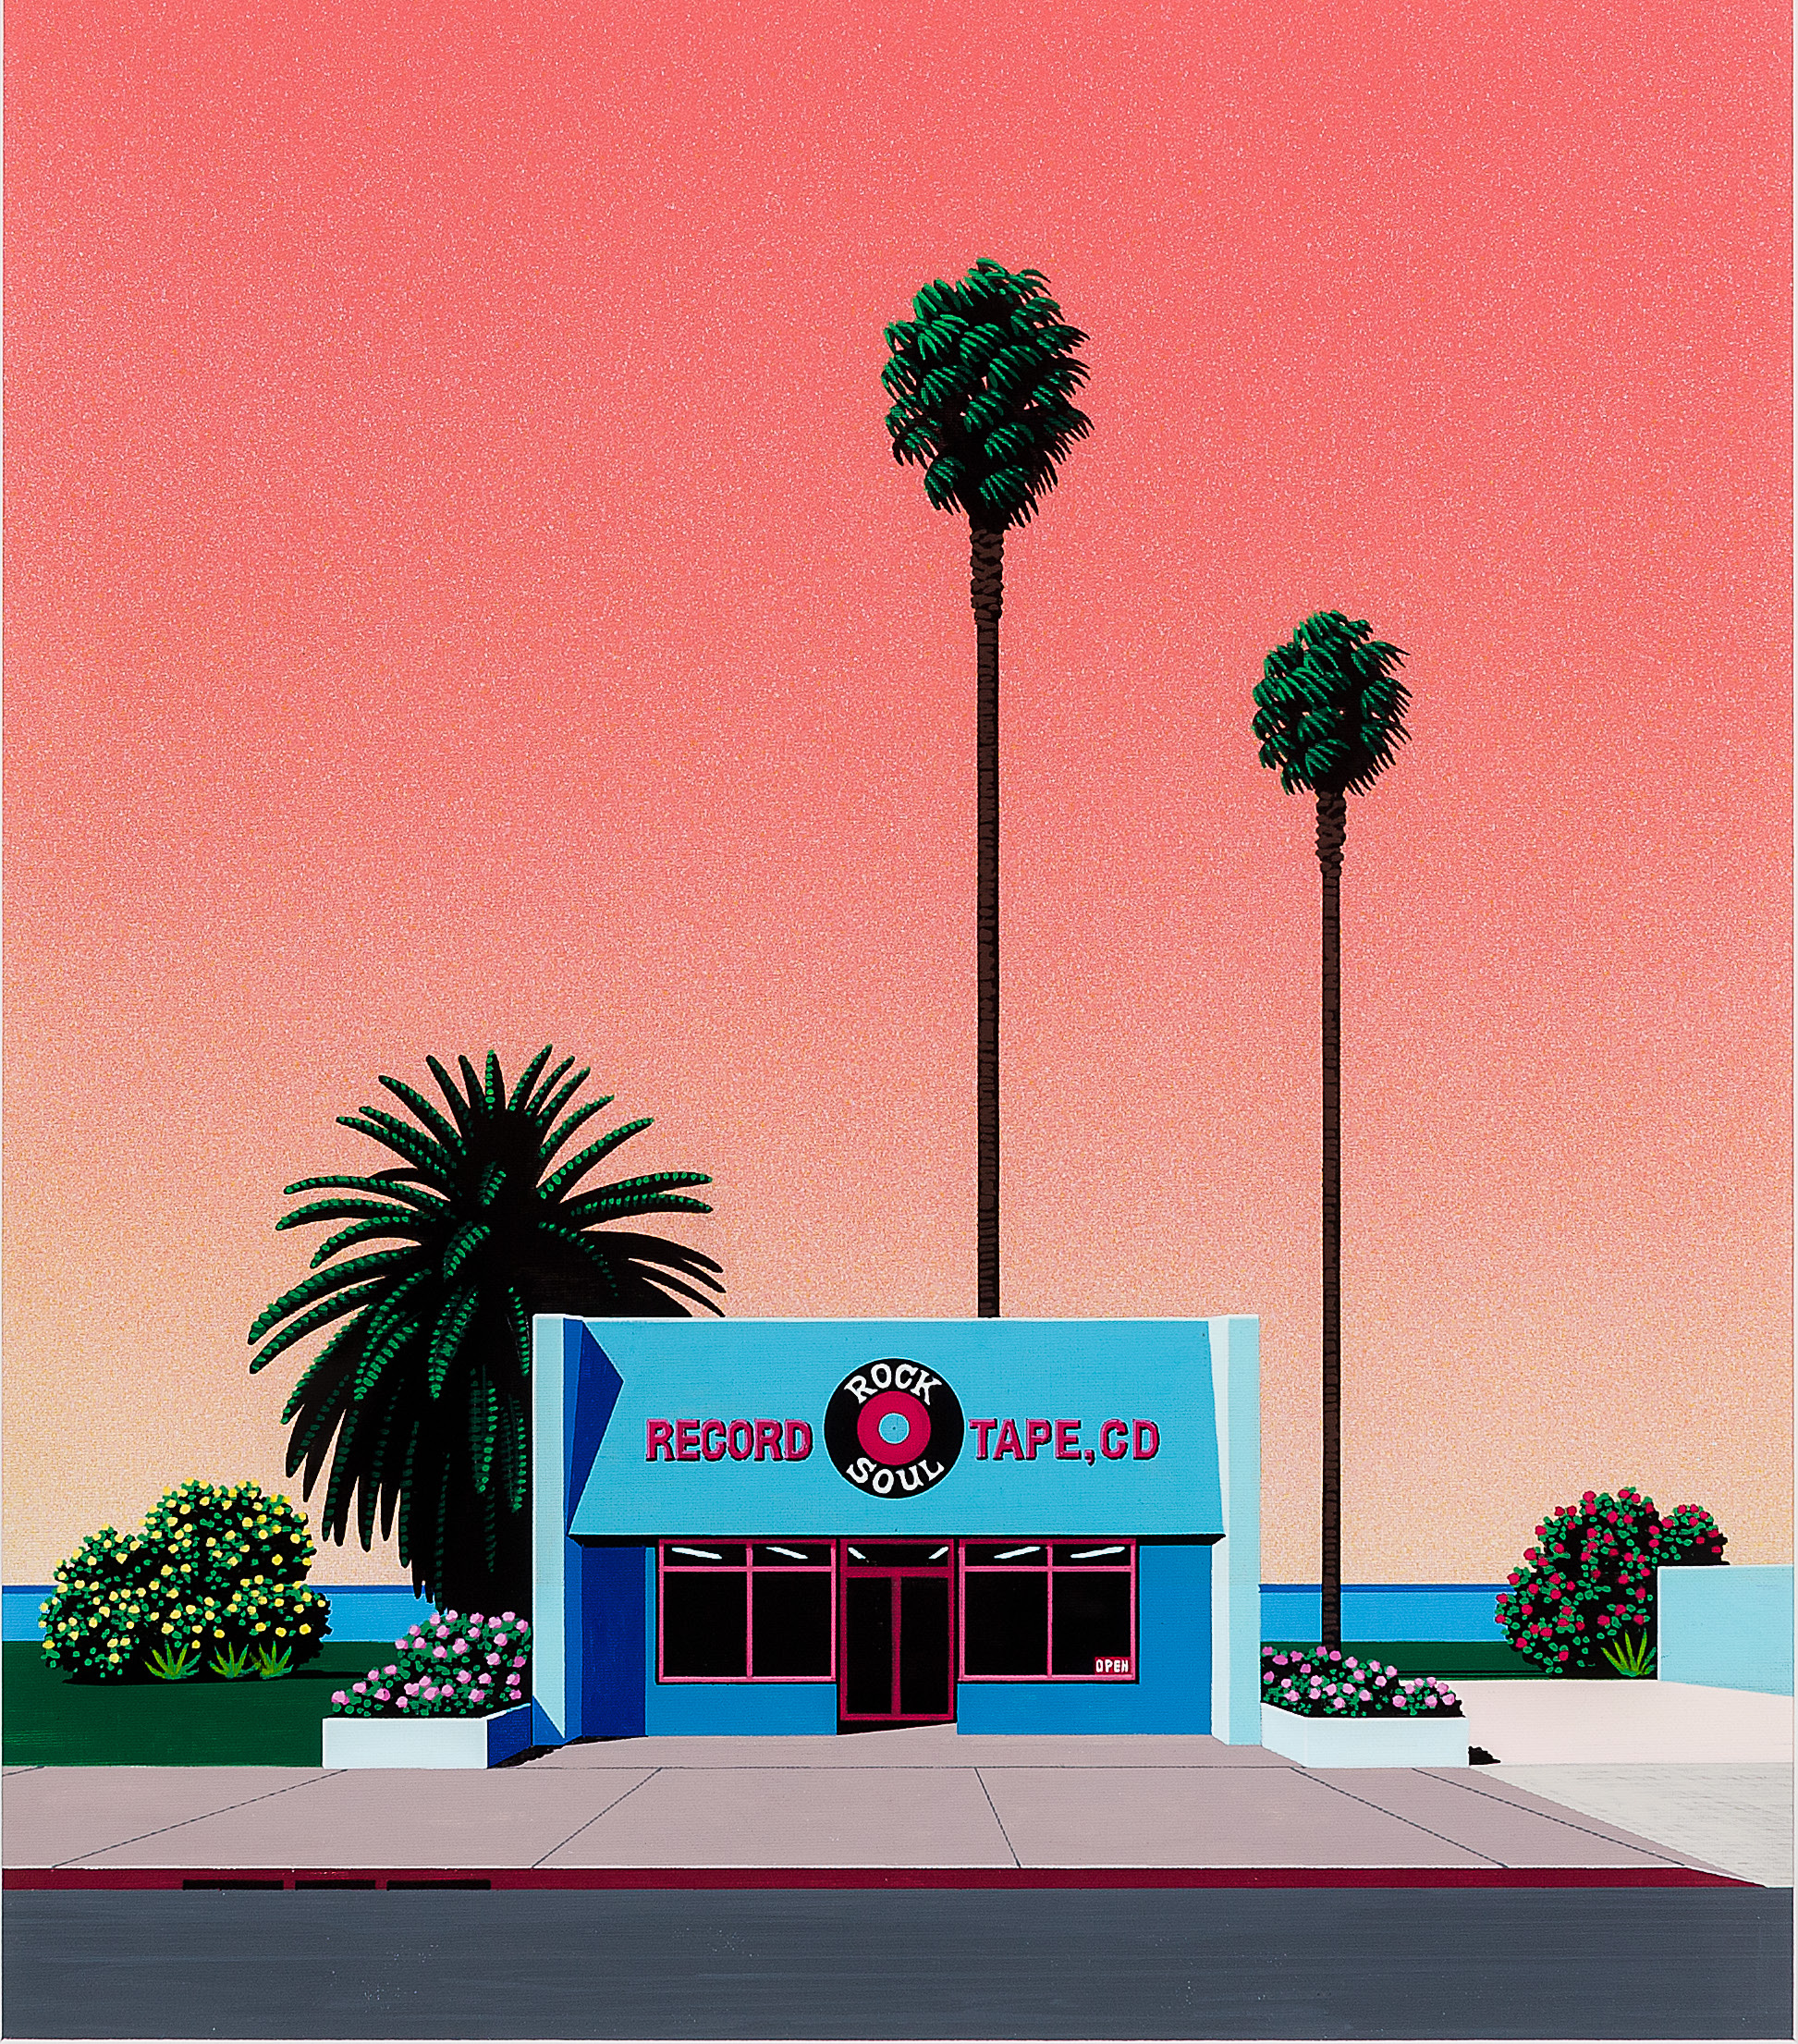
\includegraphics[width=0.52083in,height=\textheight,keepaspectratio]{img/jpf/24.jpg}
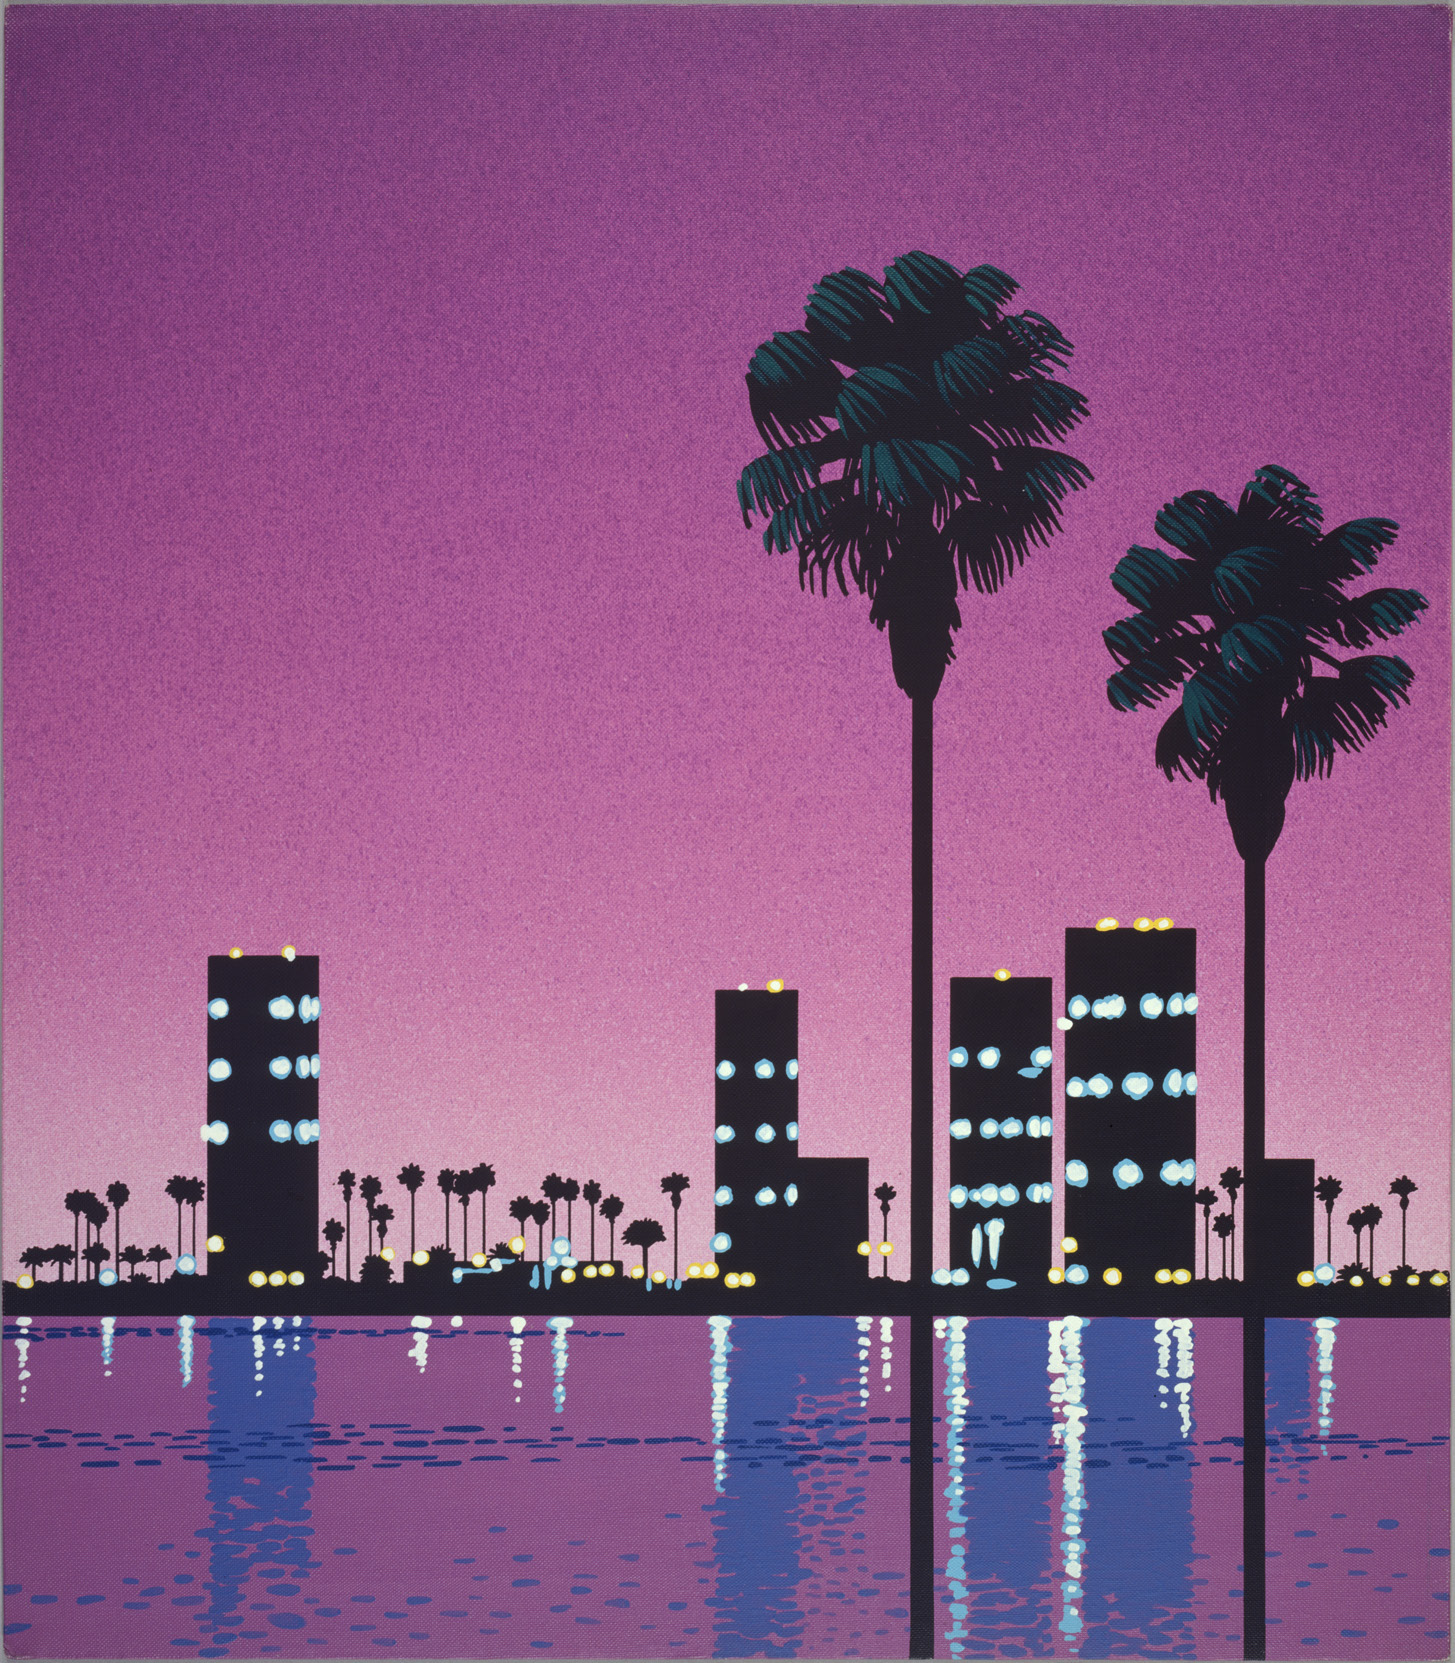
\includegraphics[width=0.52083in,height=\textheight,keepaspectratio]{img/jpf/25.jpg}
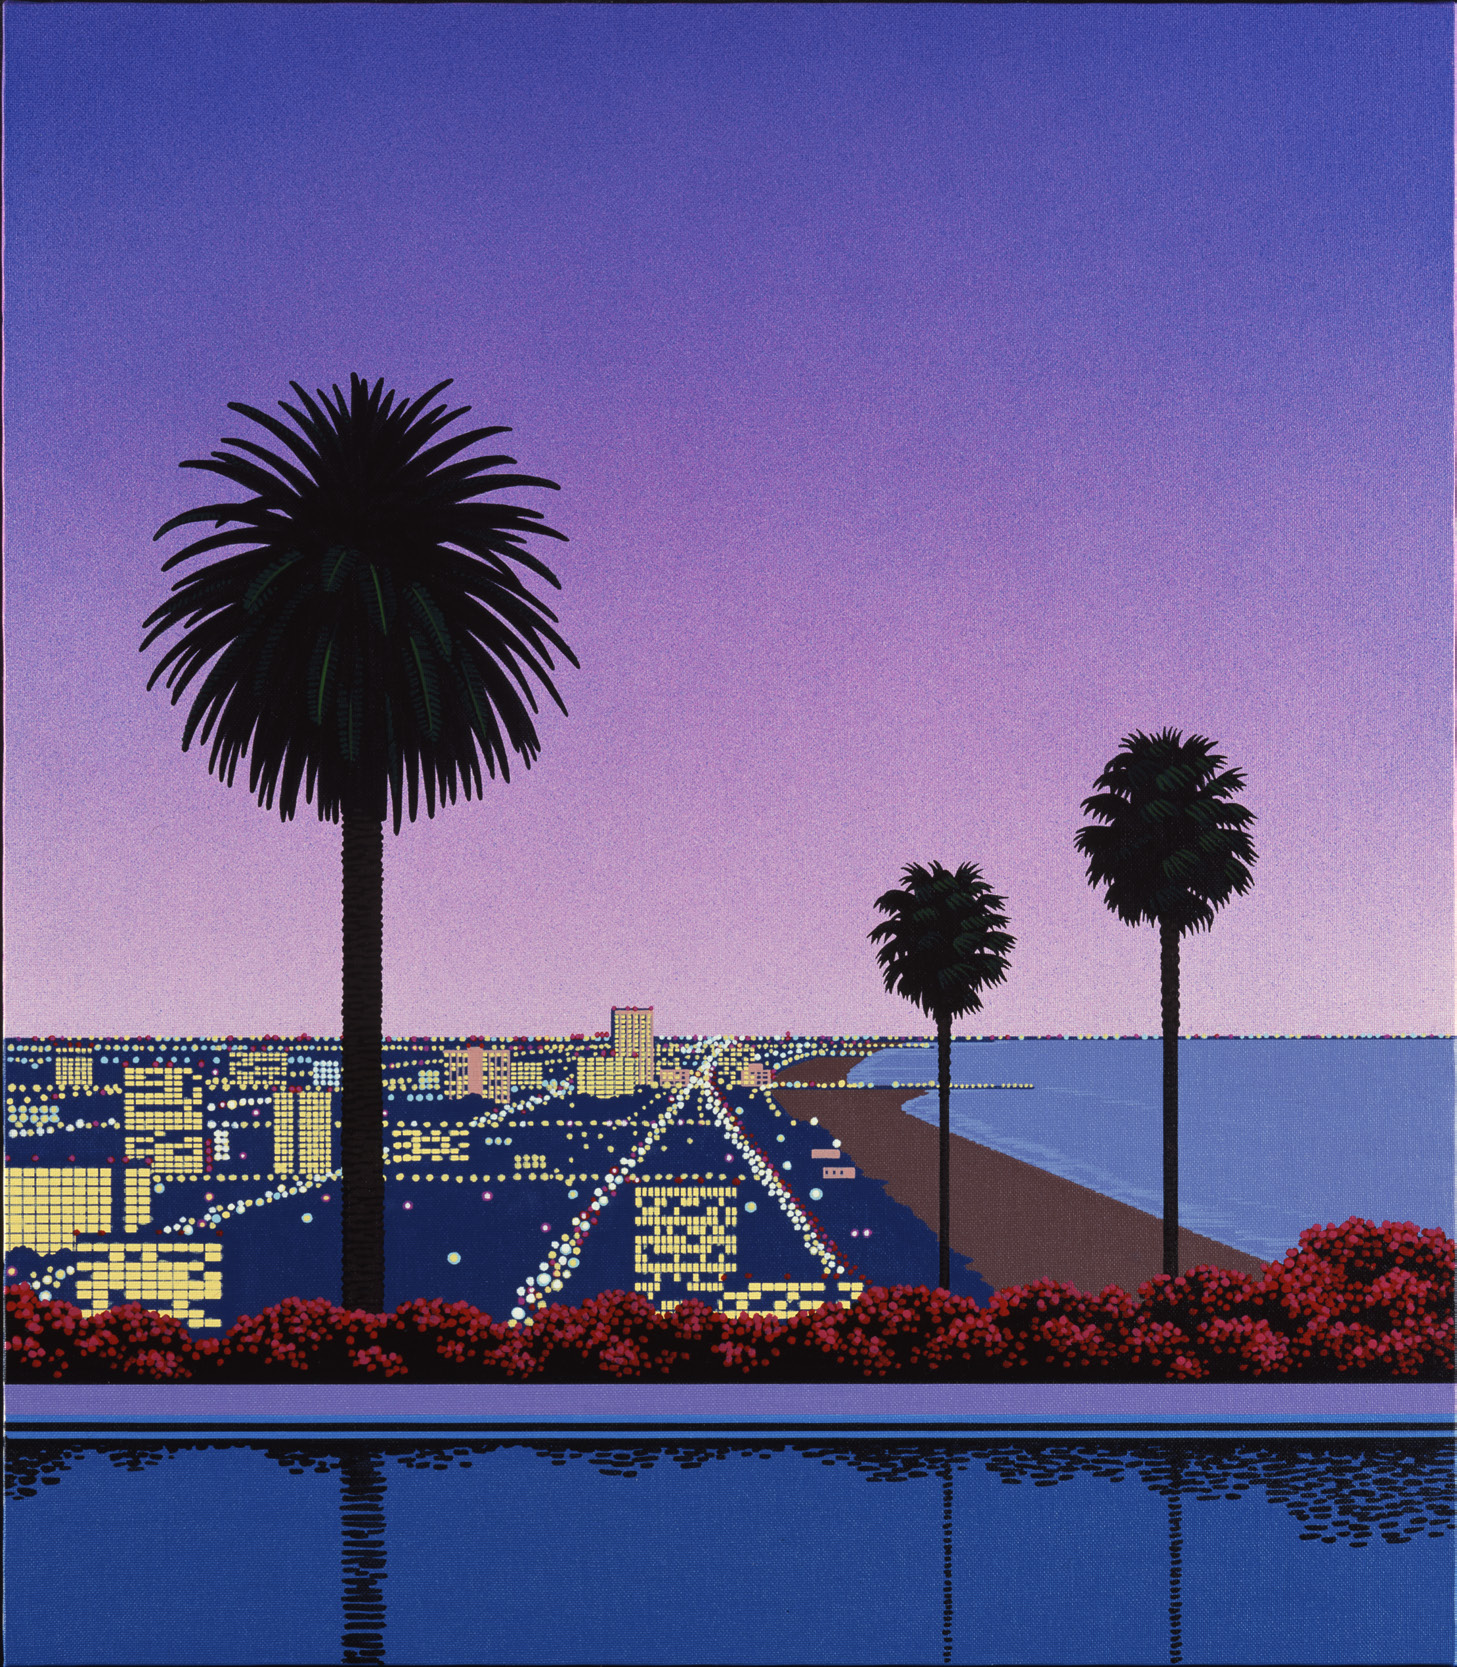
\includegraphics[width=0.52083in,height=\textheight,keepaspectratio]{img/jpf/26.jpg}
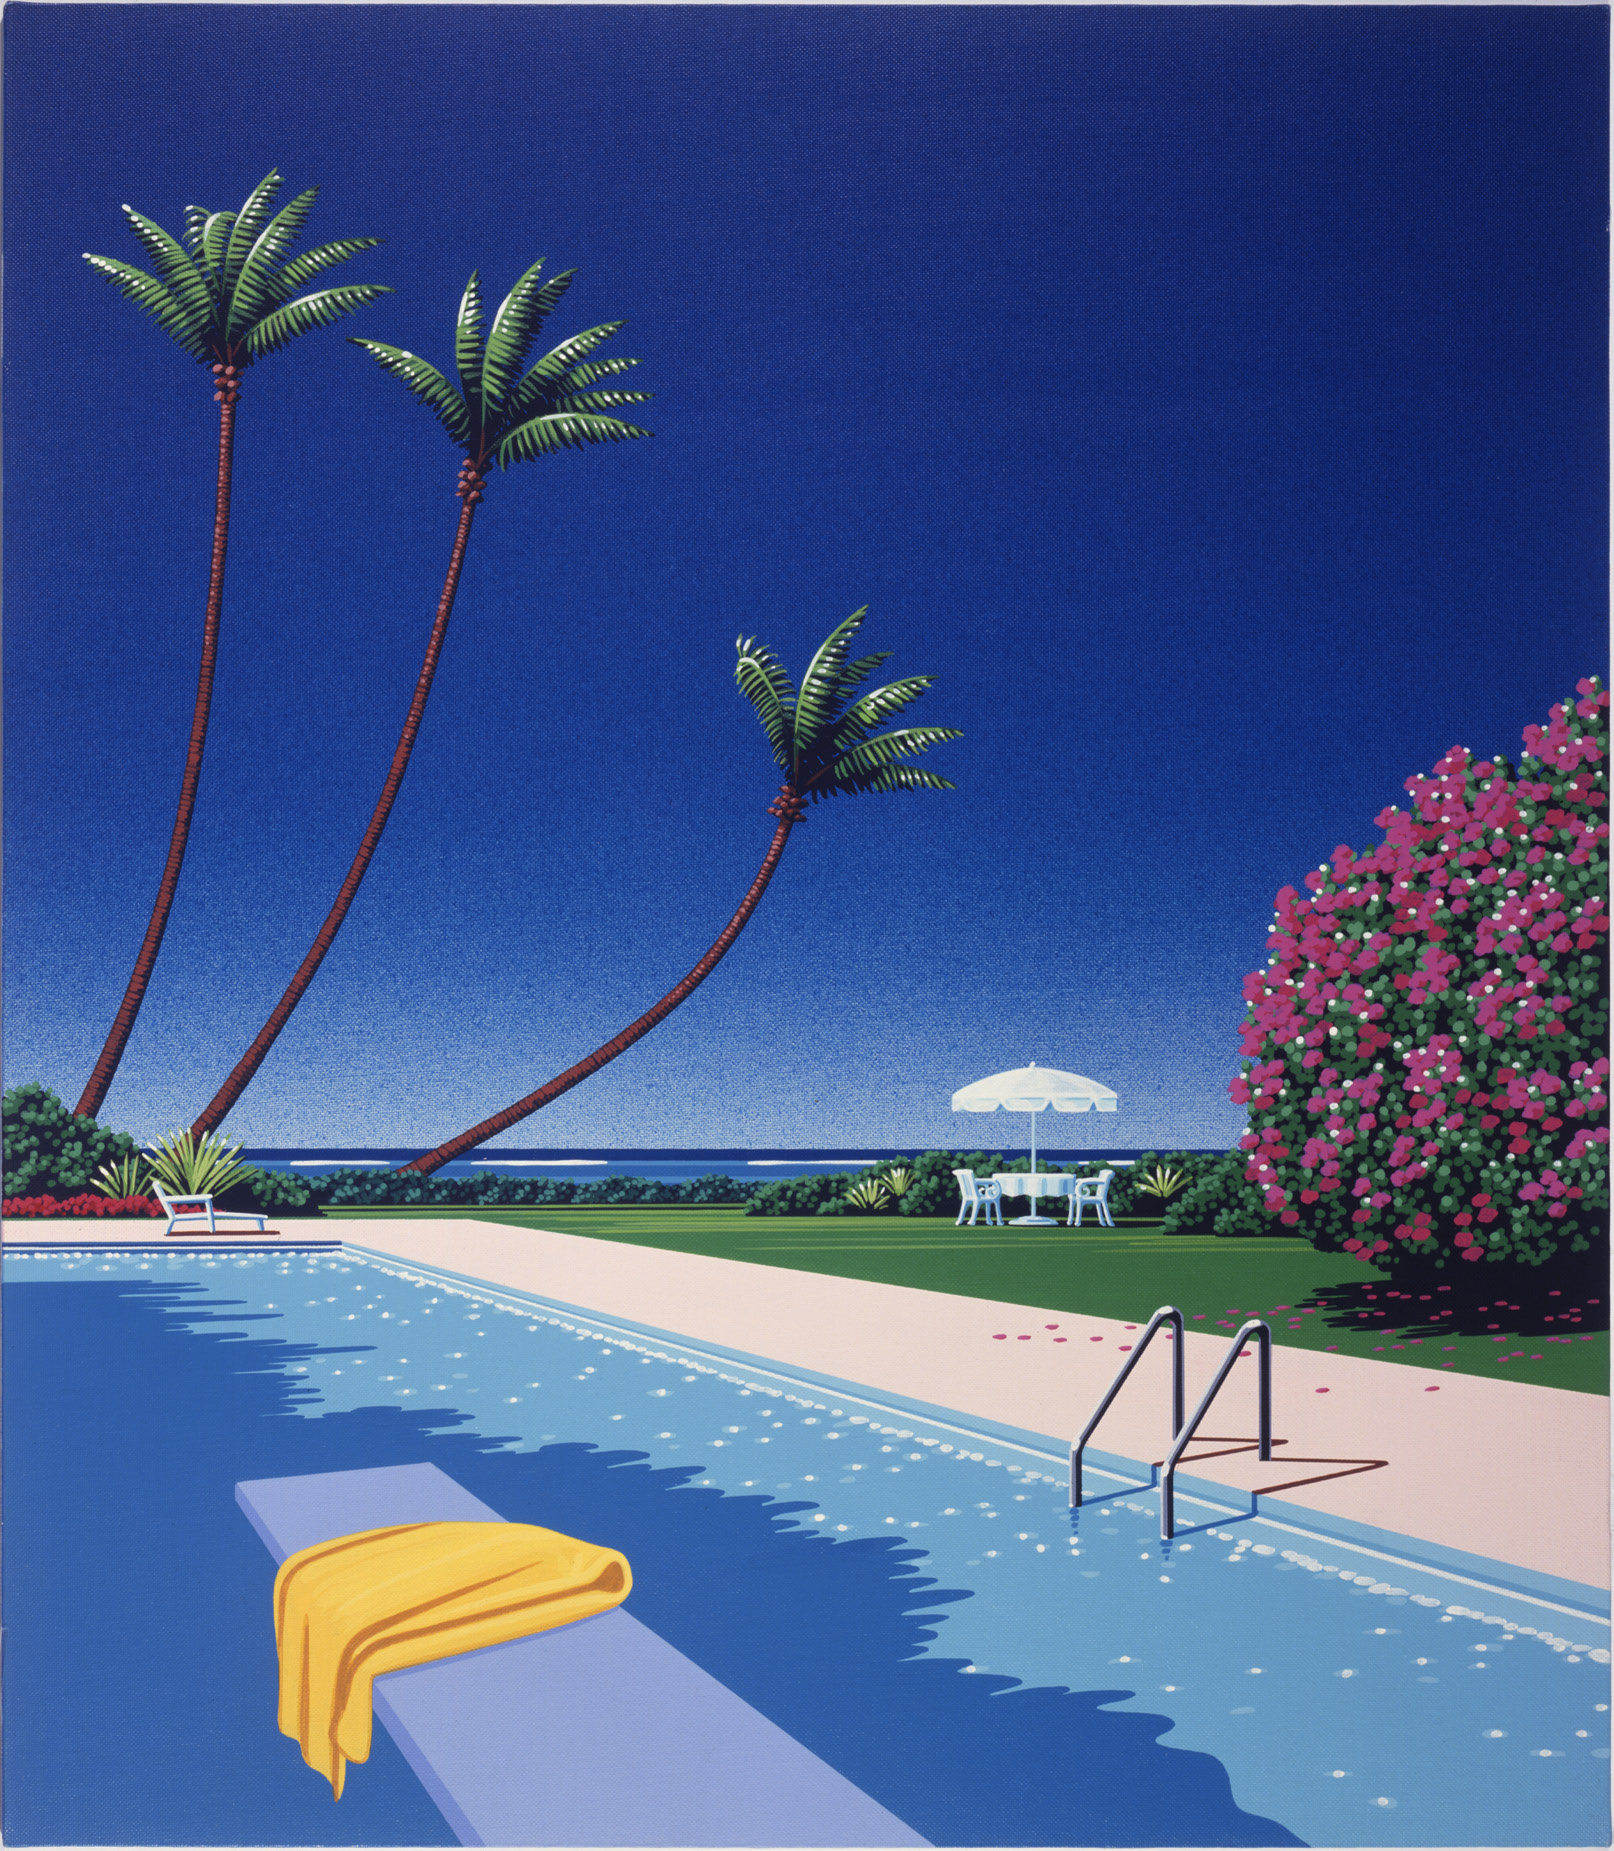
\includegraphics[width=0.52083in,height=\textheight,keepaspectratio]{img/jpf/27.jpg}
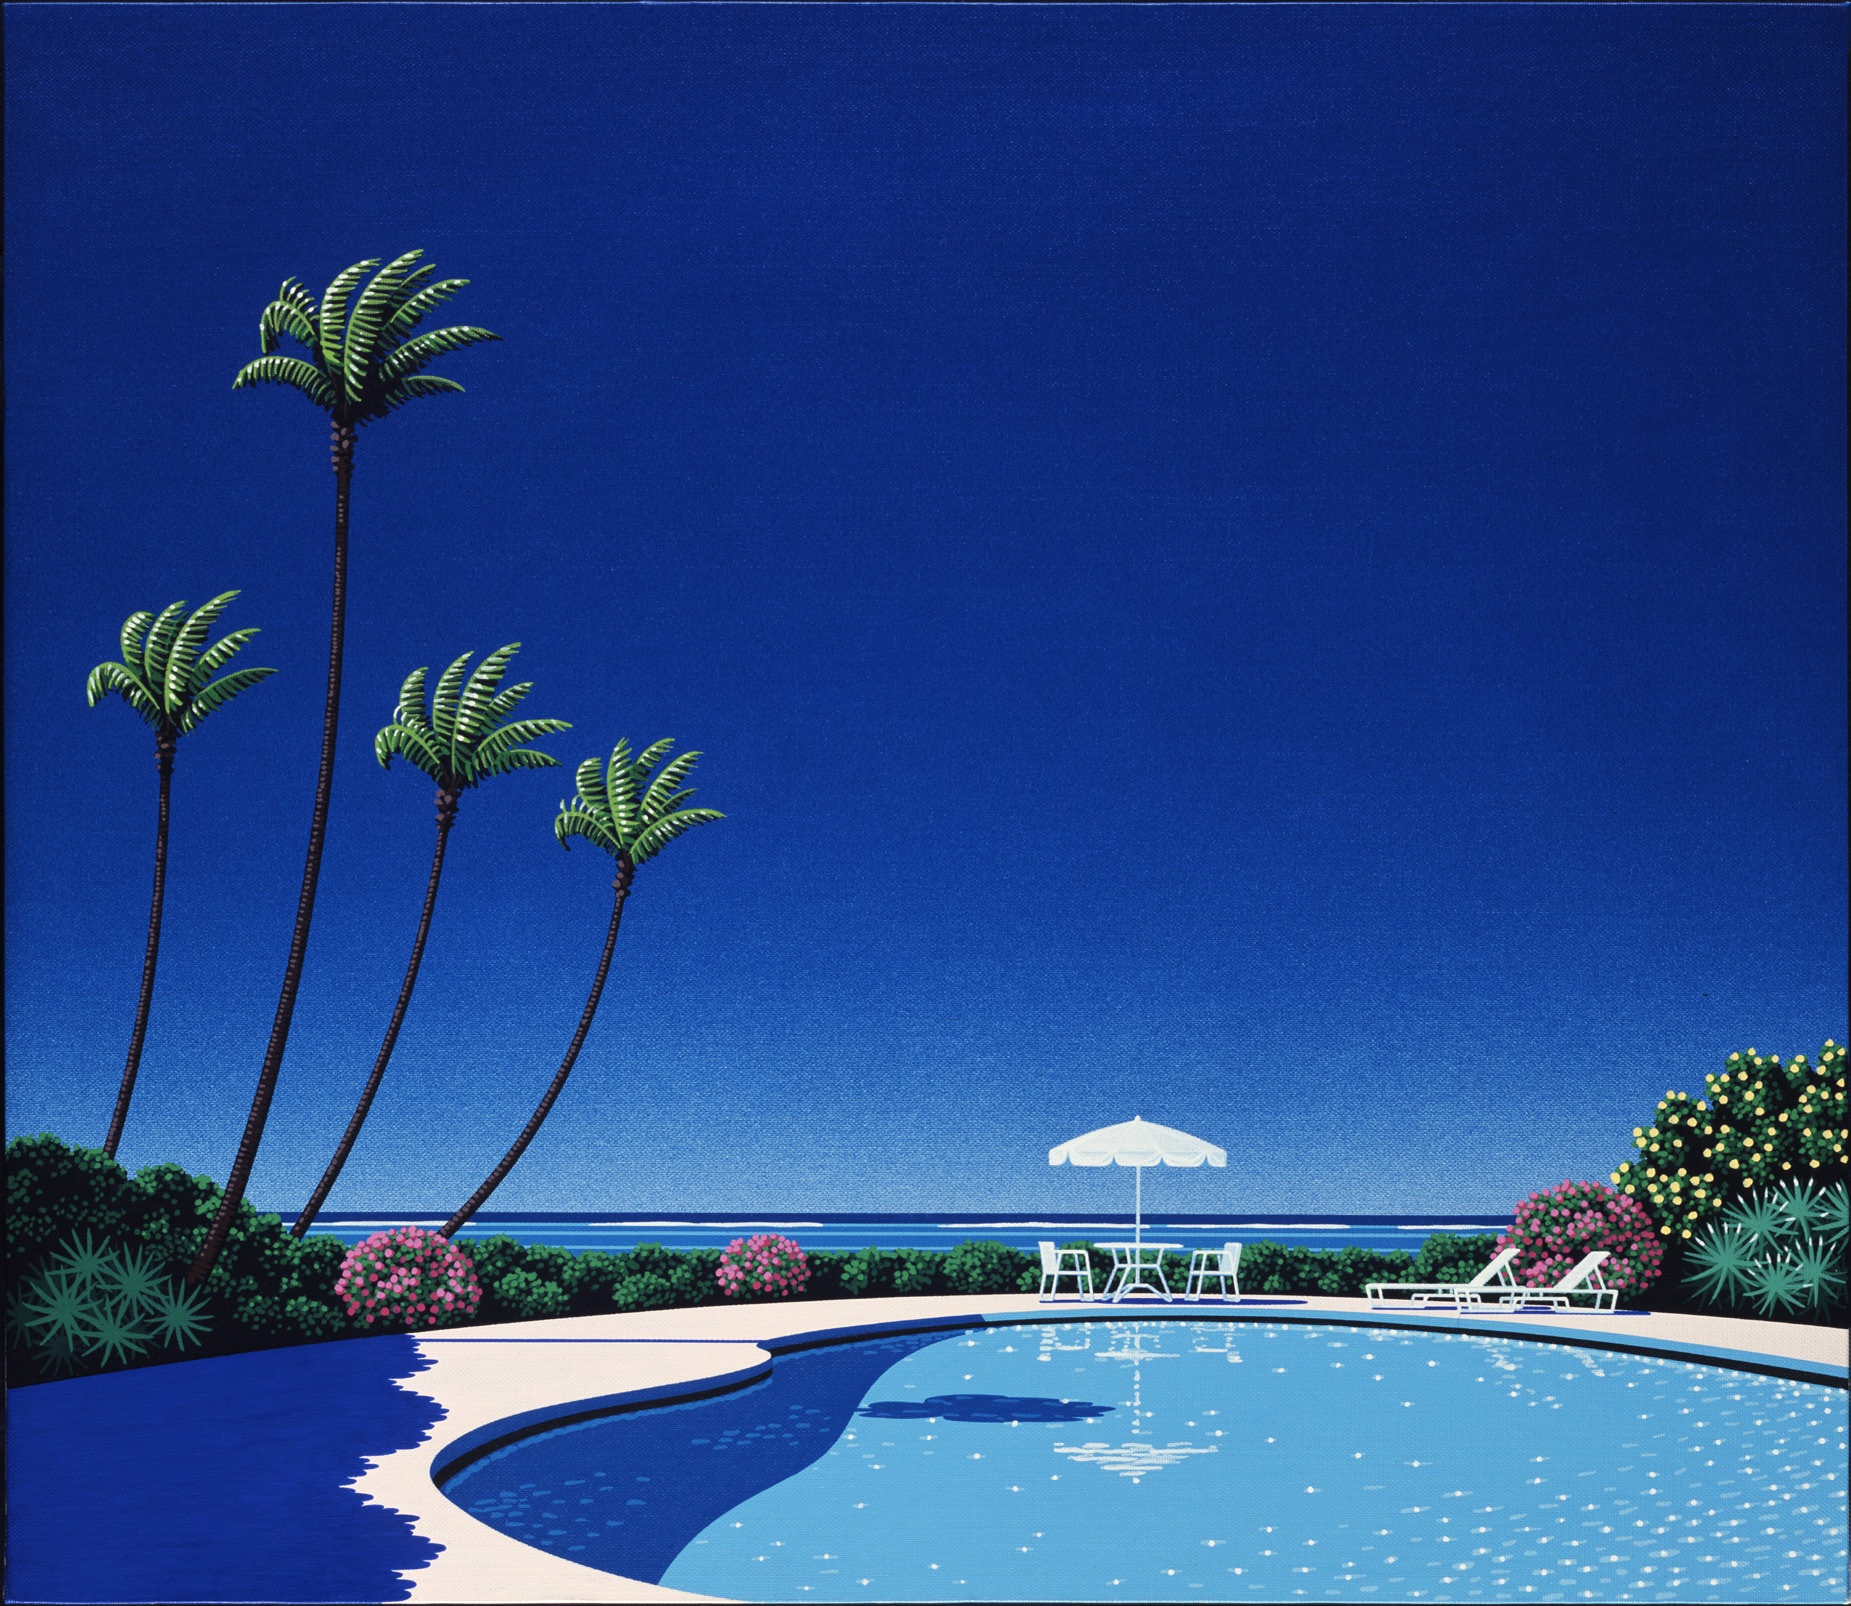
\includegraphics[width=0.52083in,height=\textheight,keepaspectratio]{img/jpf/28.jpg}
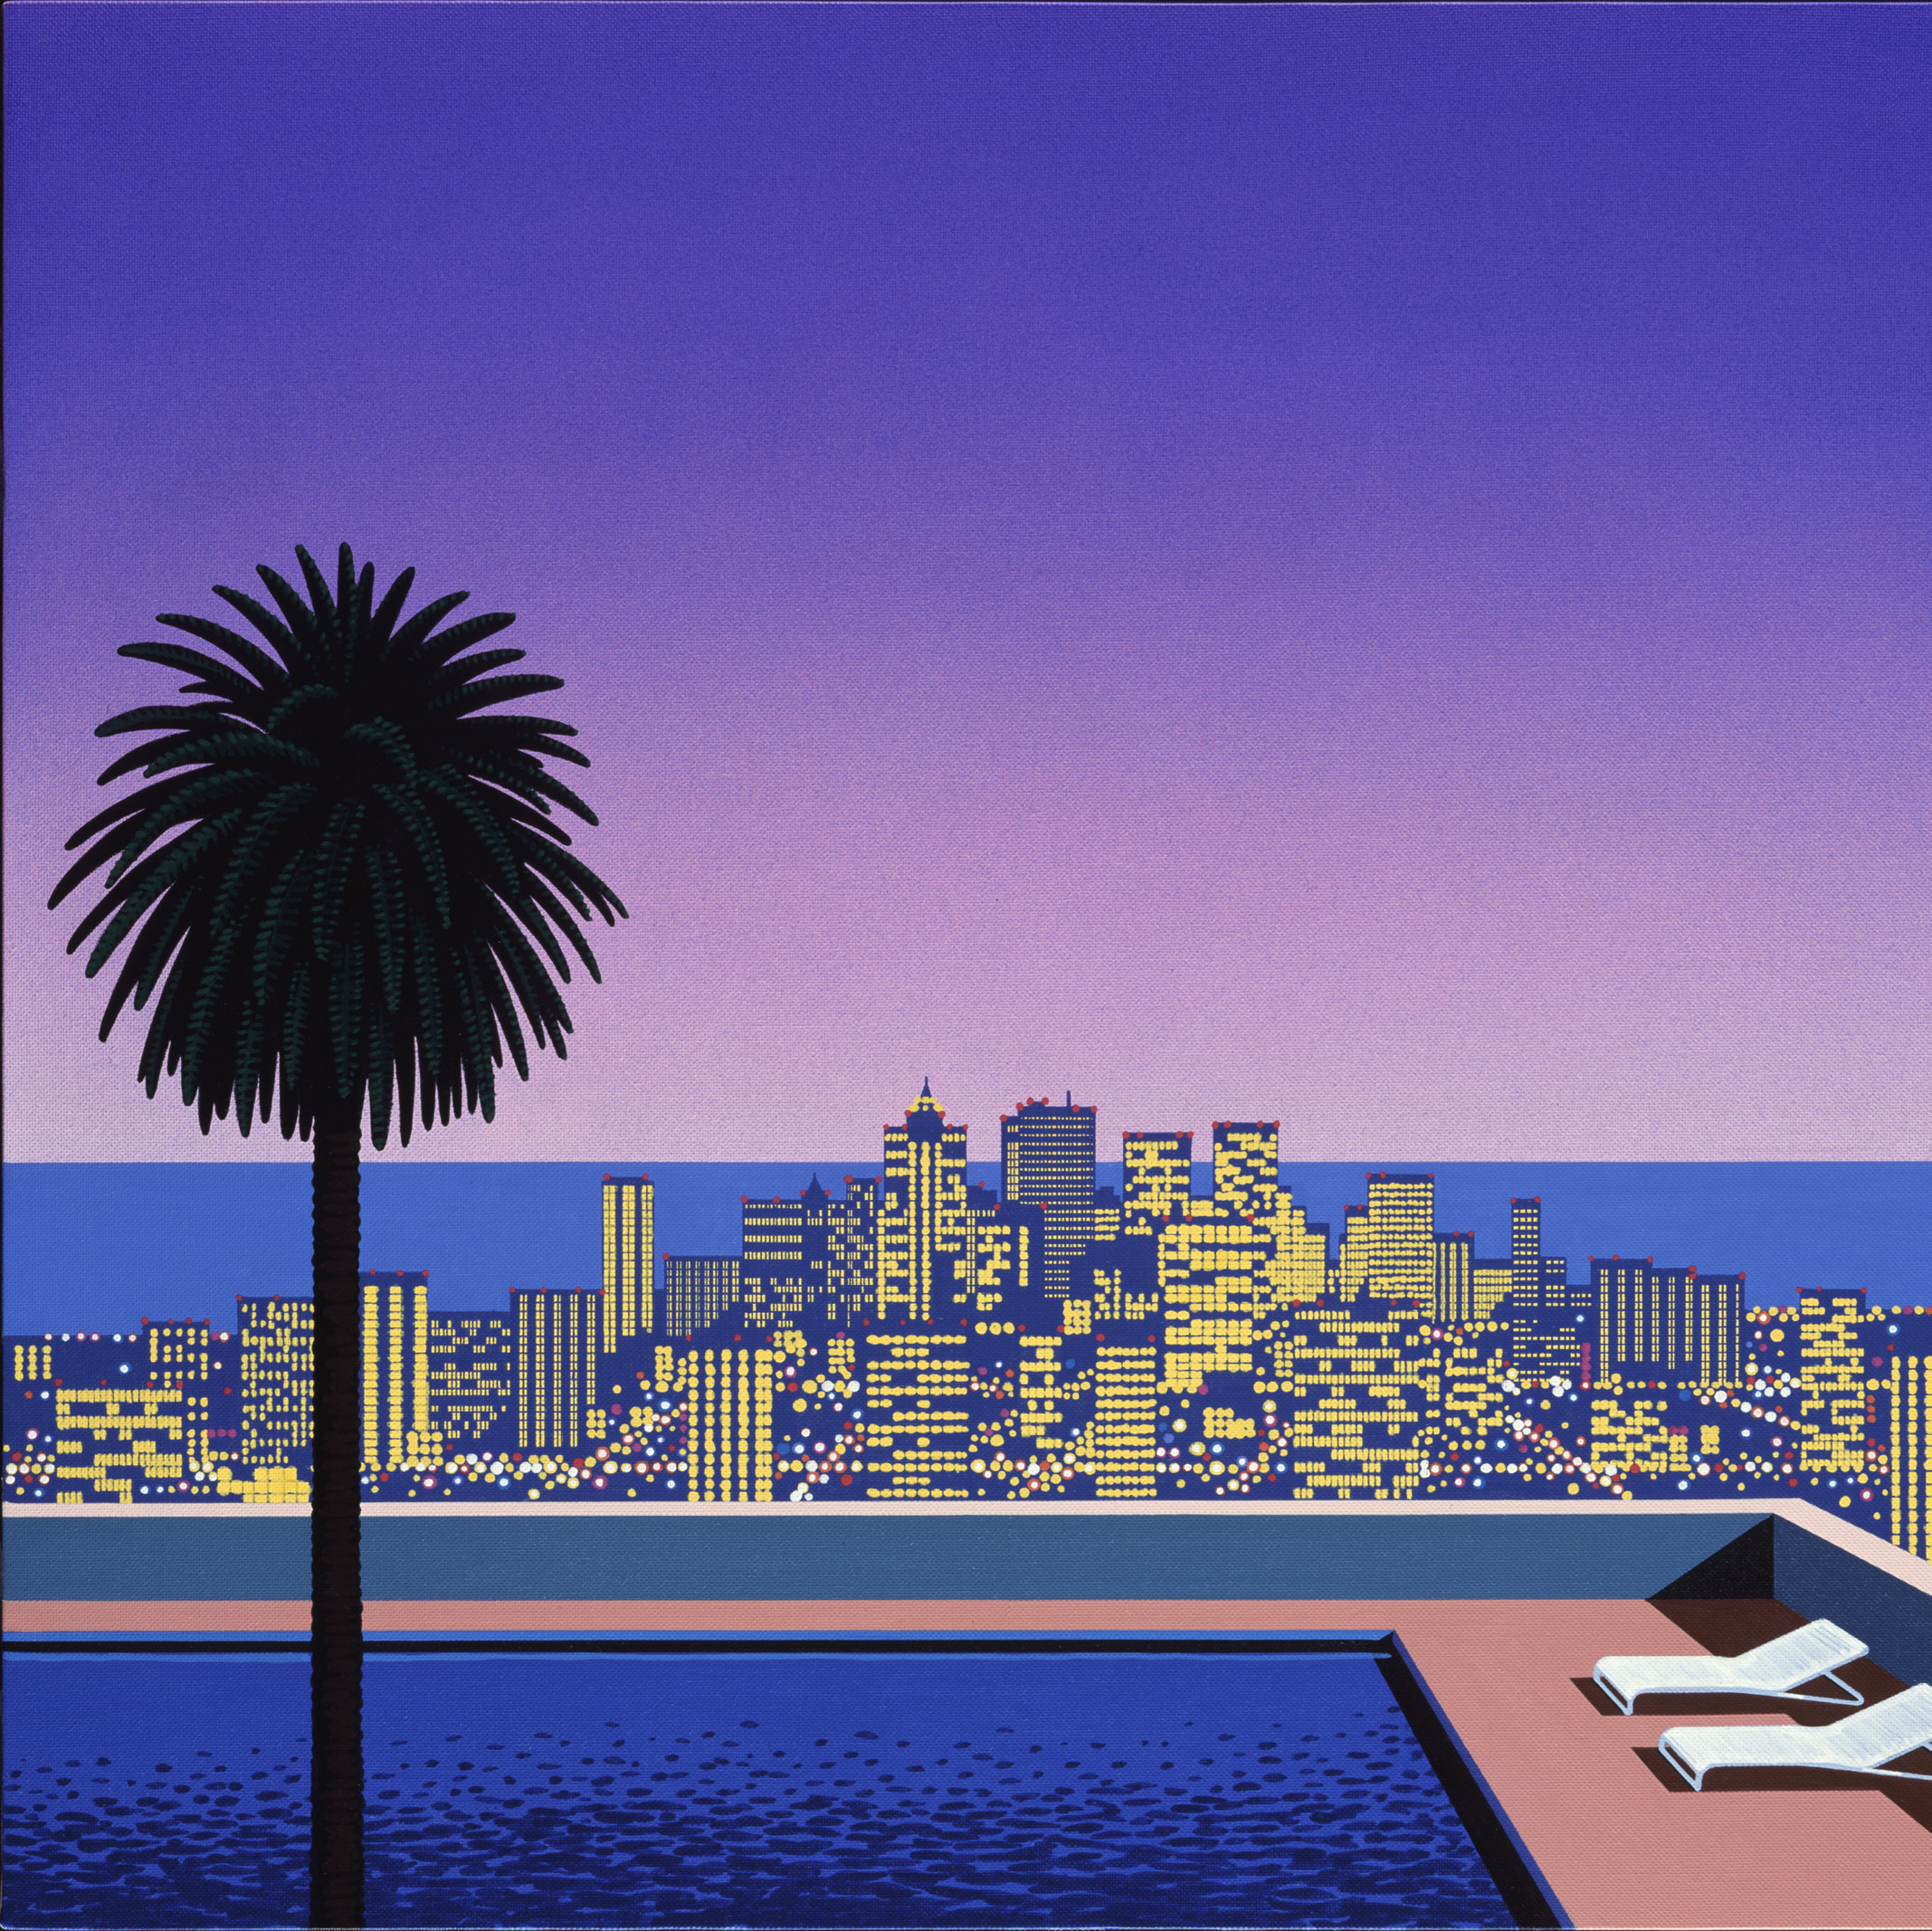
\includegraphics[width=0.52083in,height=\textheight,keepaspectratio]{img/jpf/29.jpg}
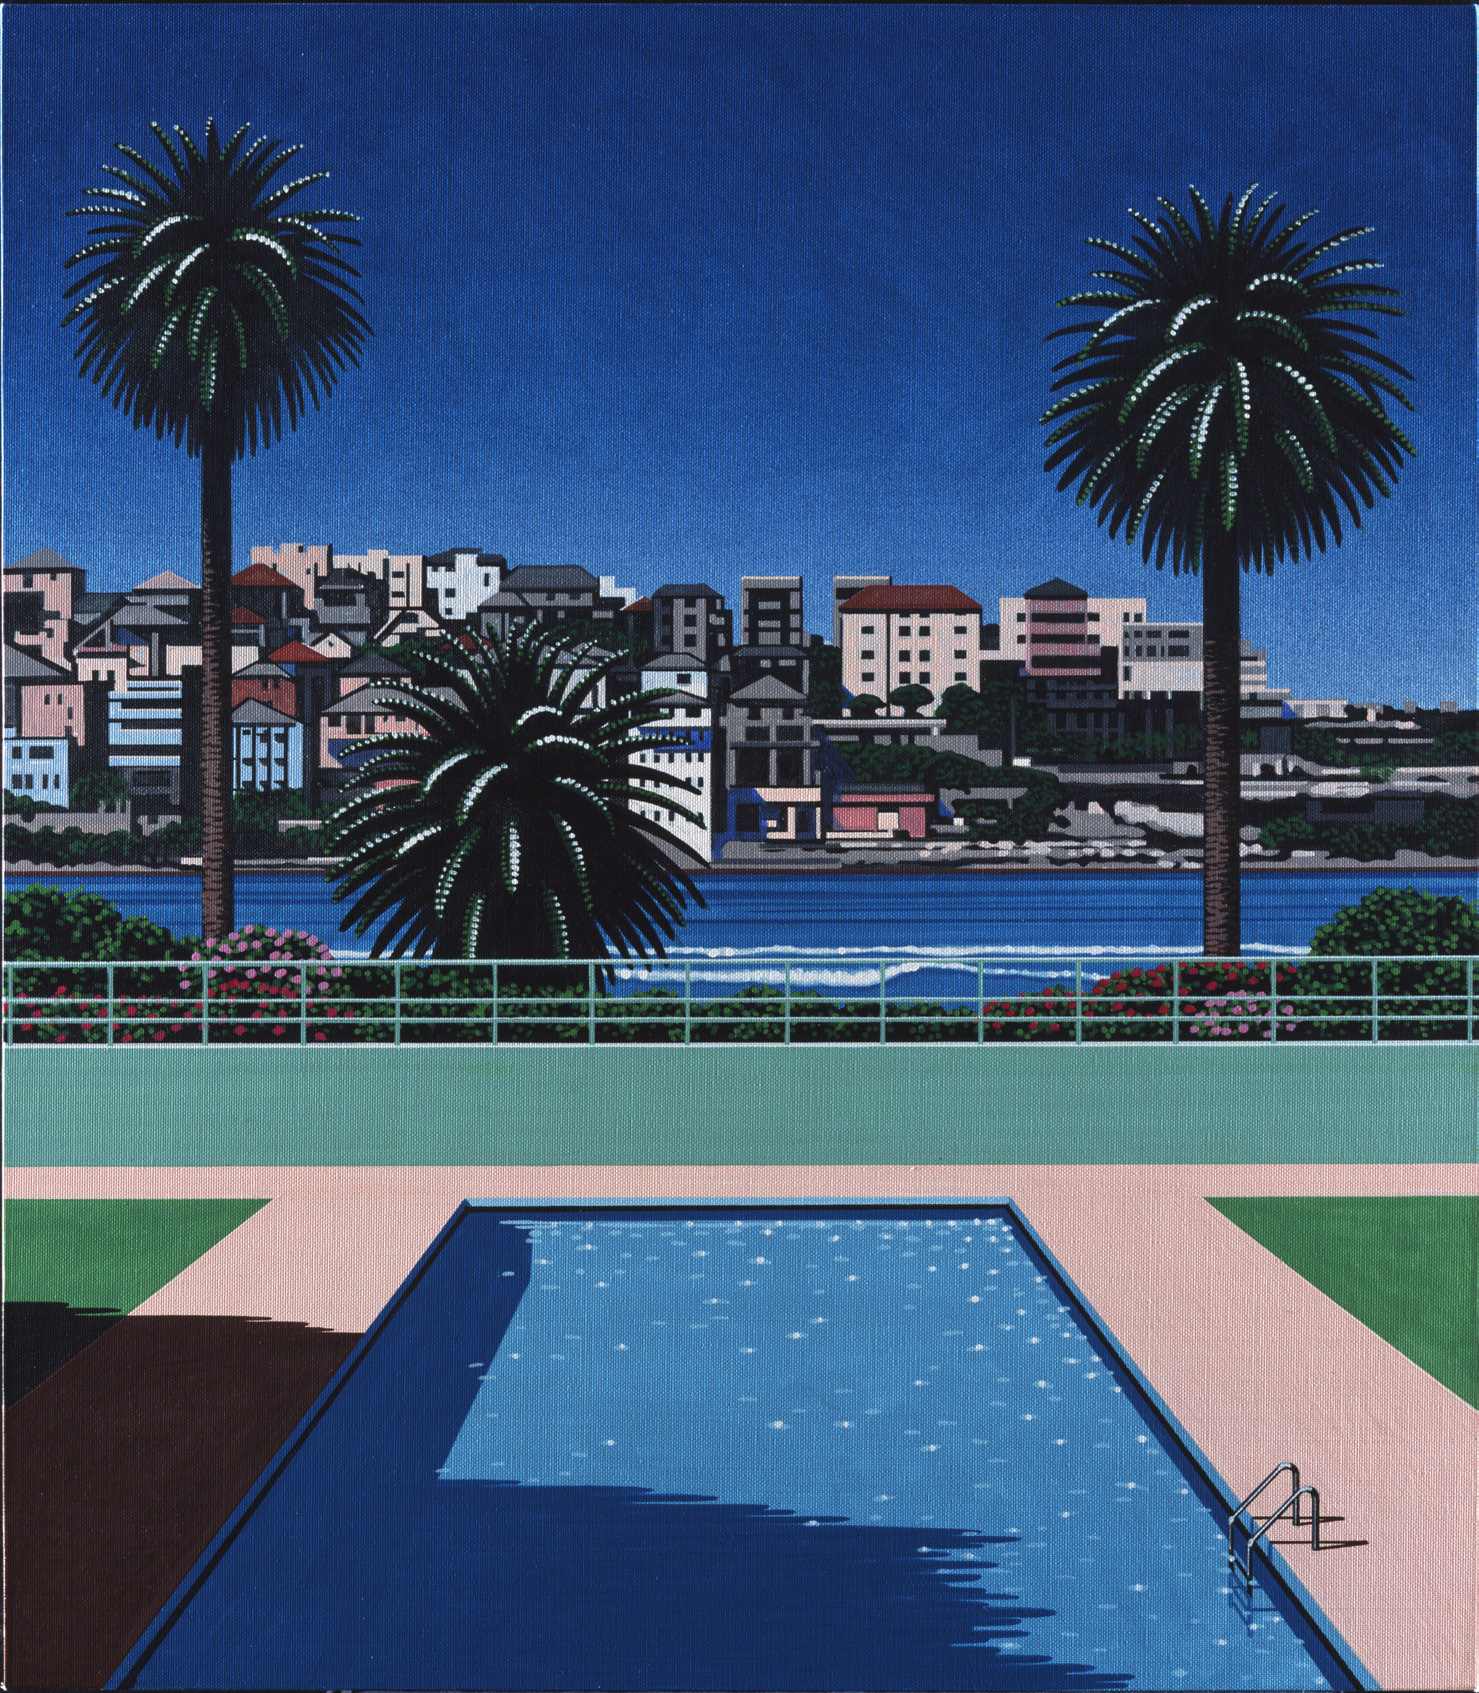
\includegraphics[width=0.52083in,height=\textheight,keepaspectratio]{img/jpf/31.jpg}
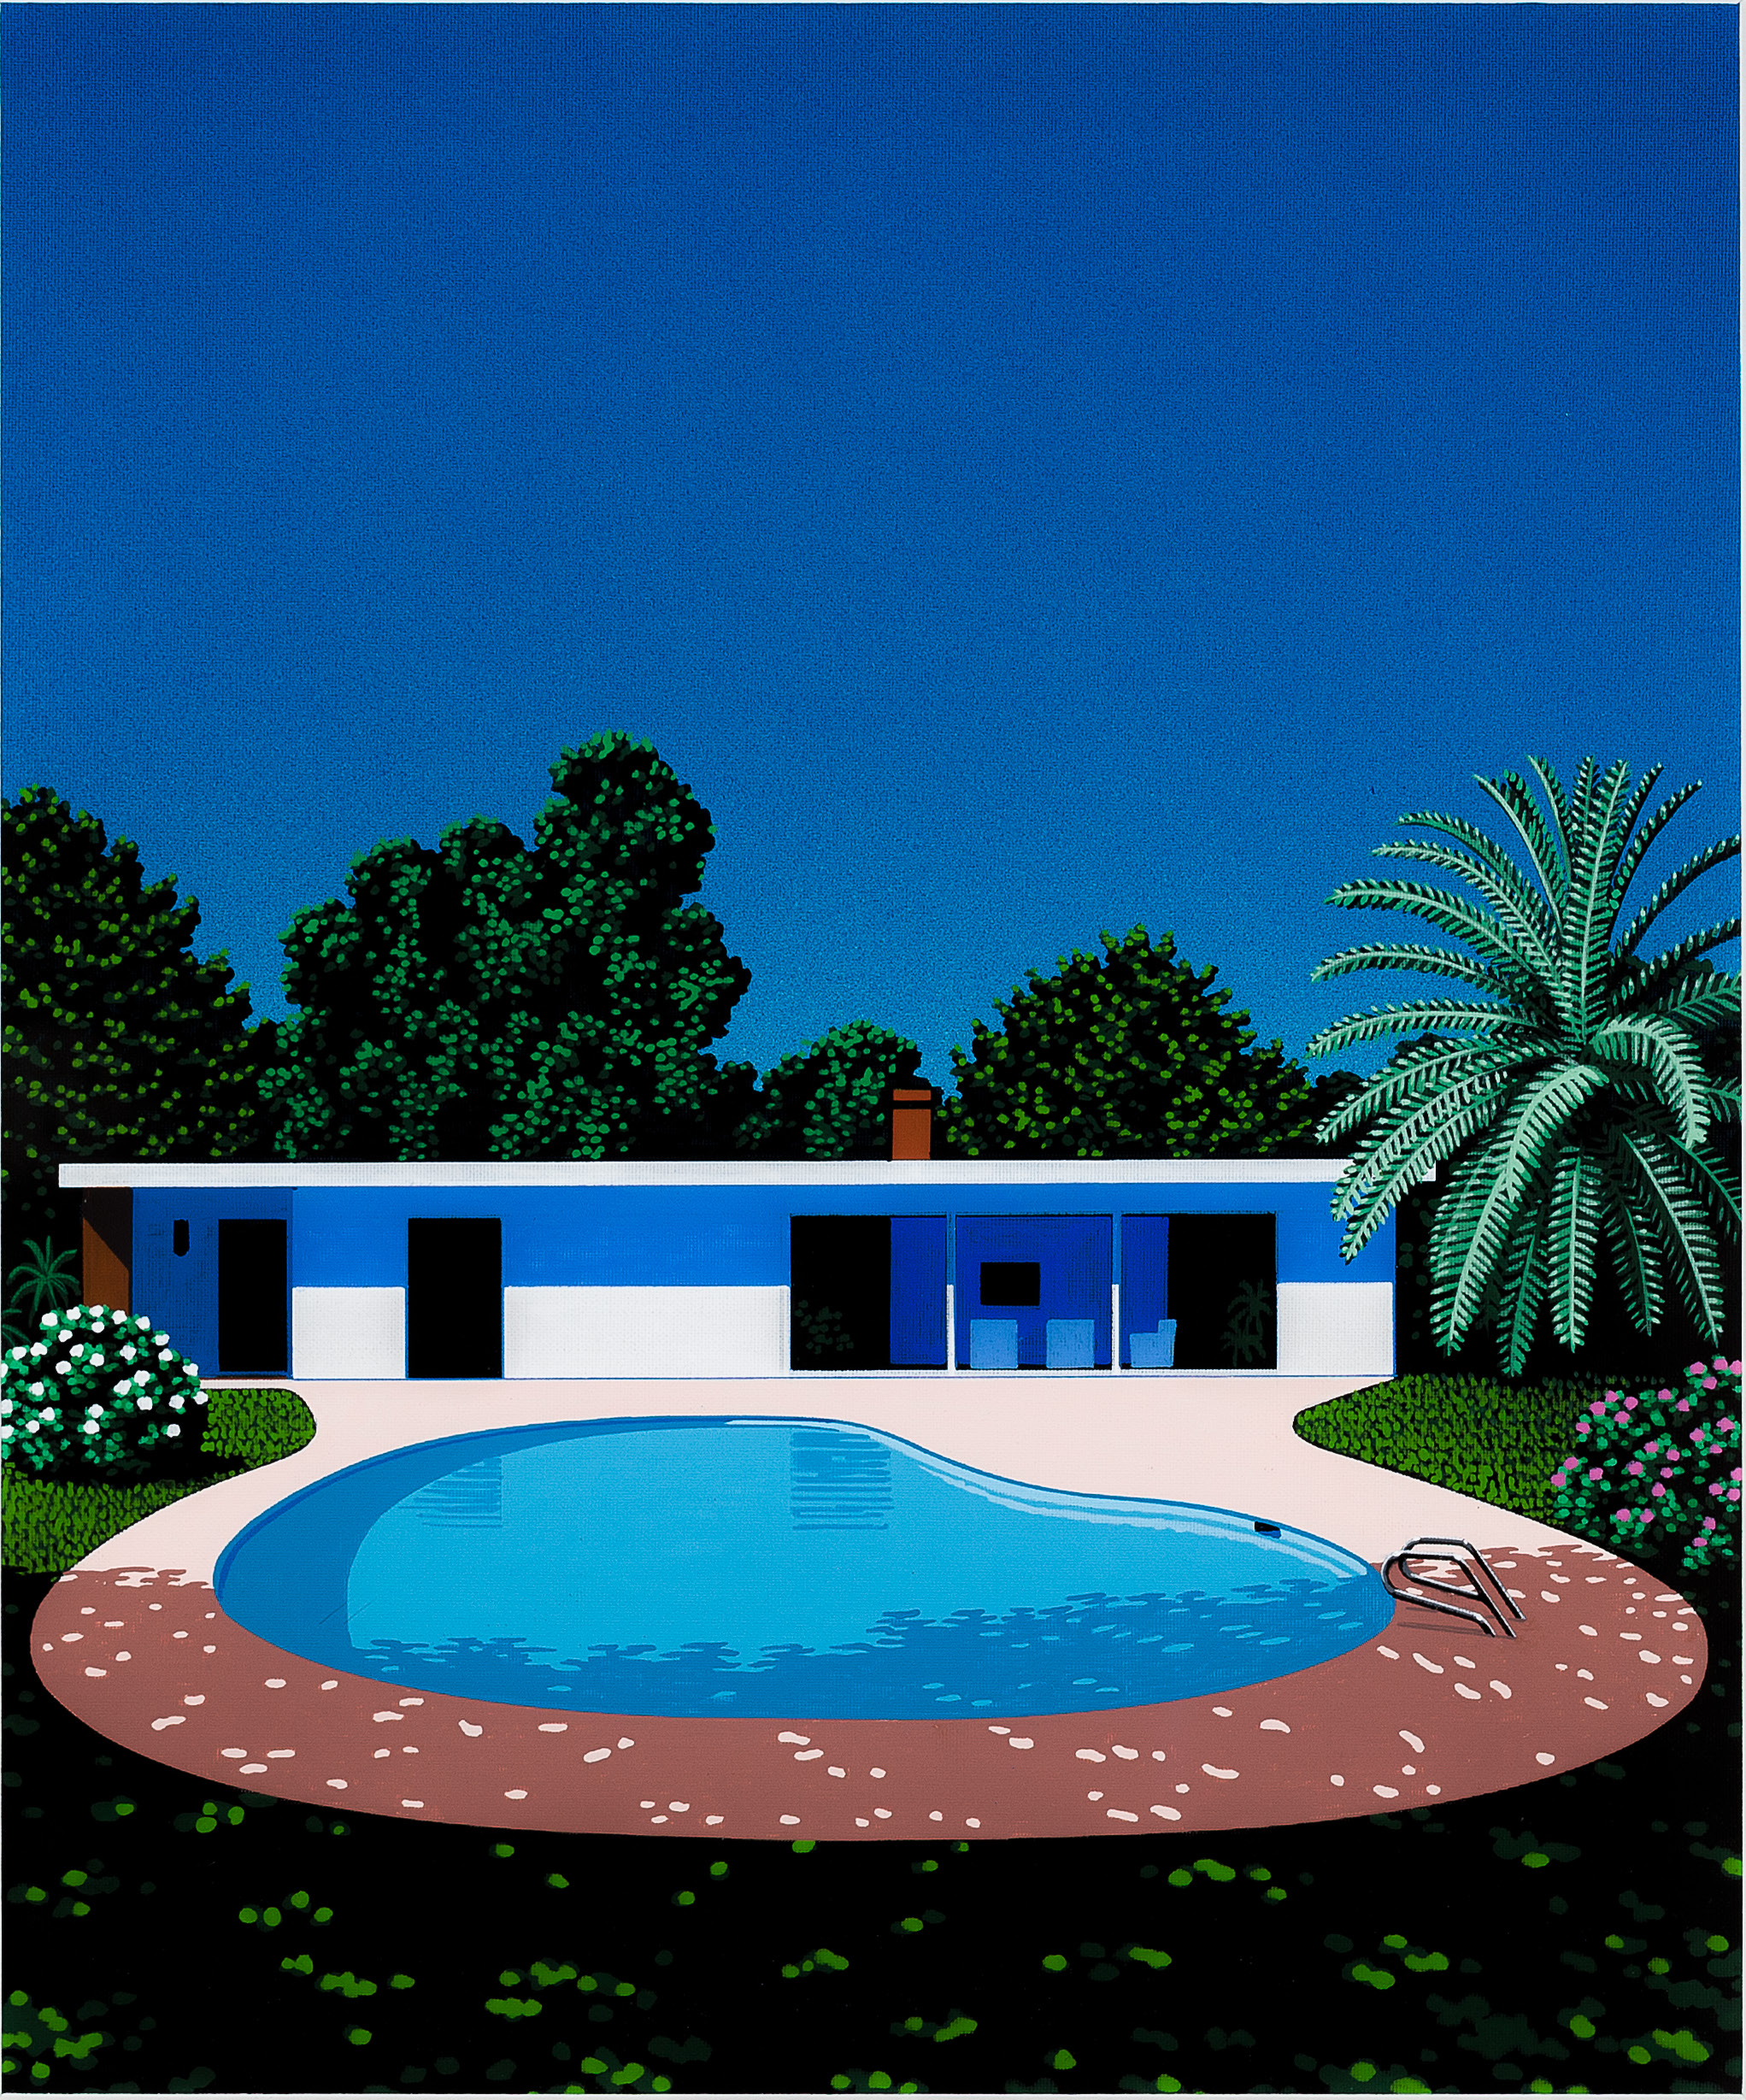
\includegraphics[width=0.52083in,height=\textheight,keepaspectratio]{img/jpf/32.jpg}
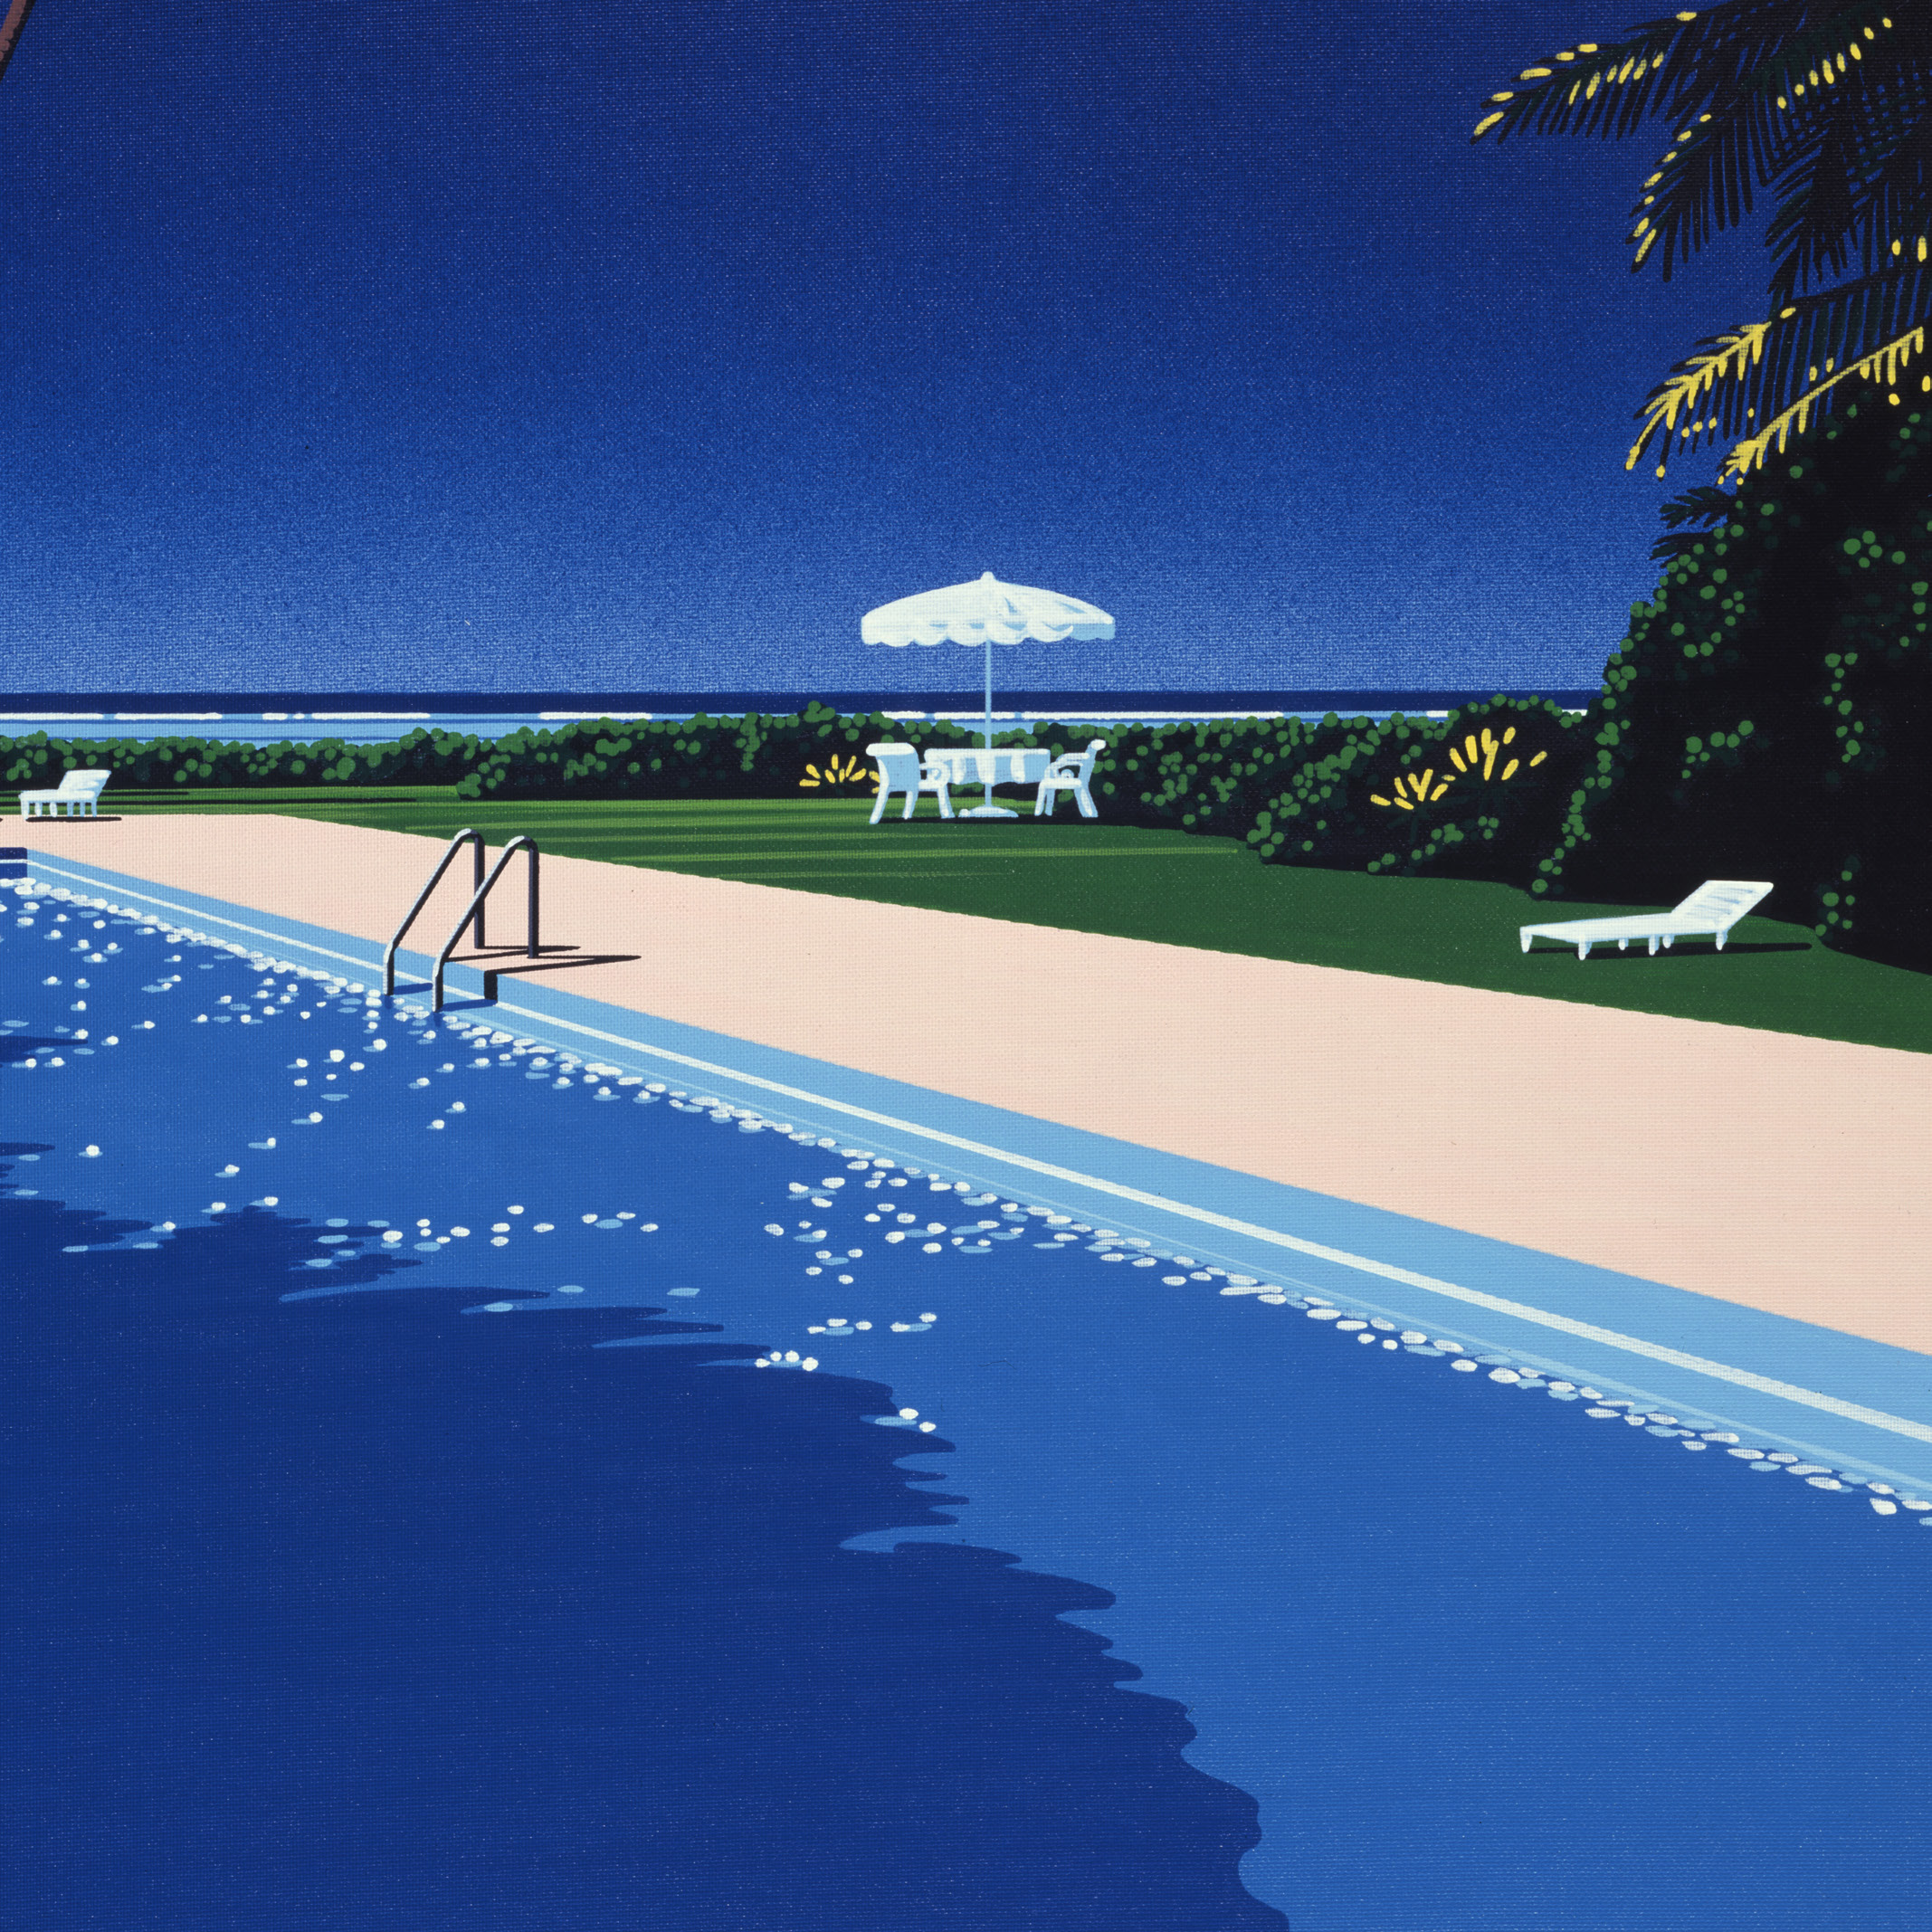
\includegraphics[width=0.52083in,height=\textheight,keepaspectratio]{img/jpf/34.jpg}
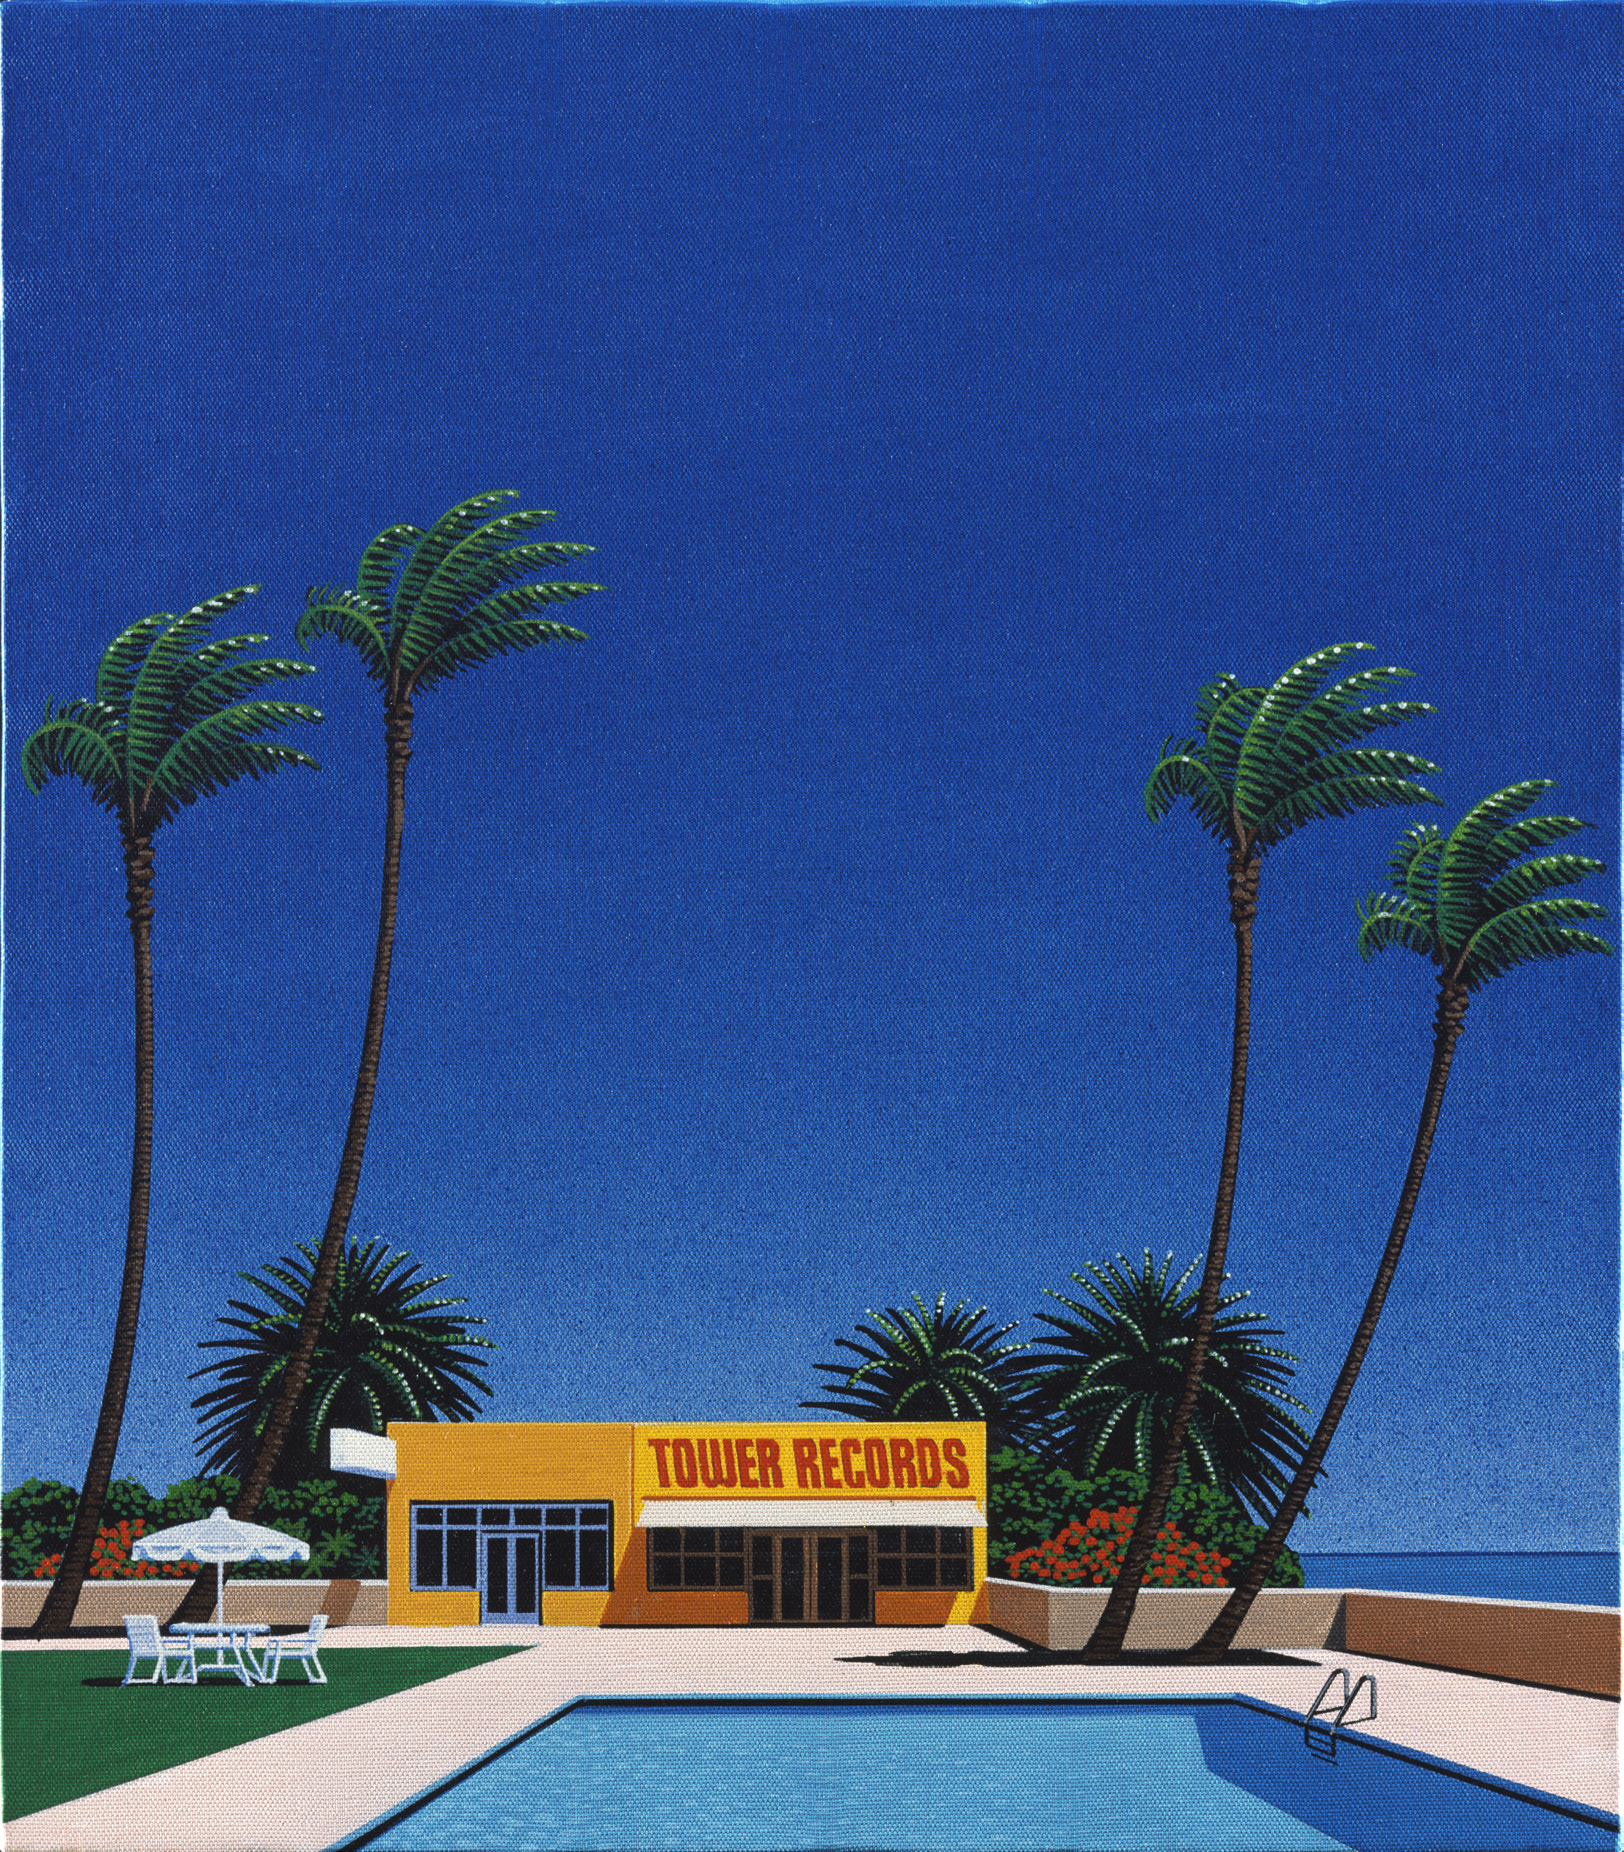
\includegraphics[width=0.52083in,height=\textheight,keepaspectratio]{img/jpf/35.jpg}
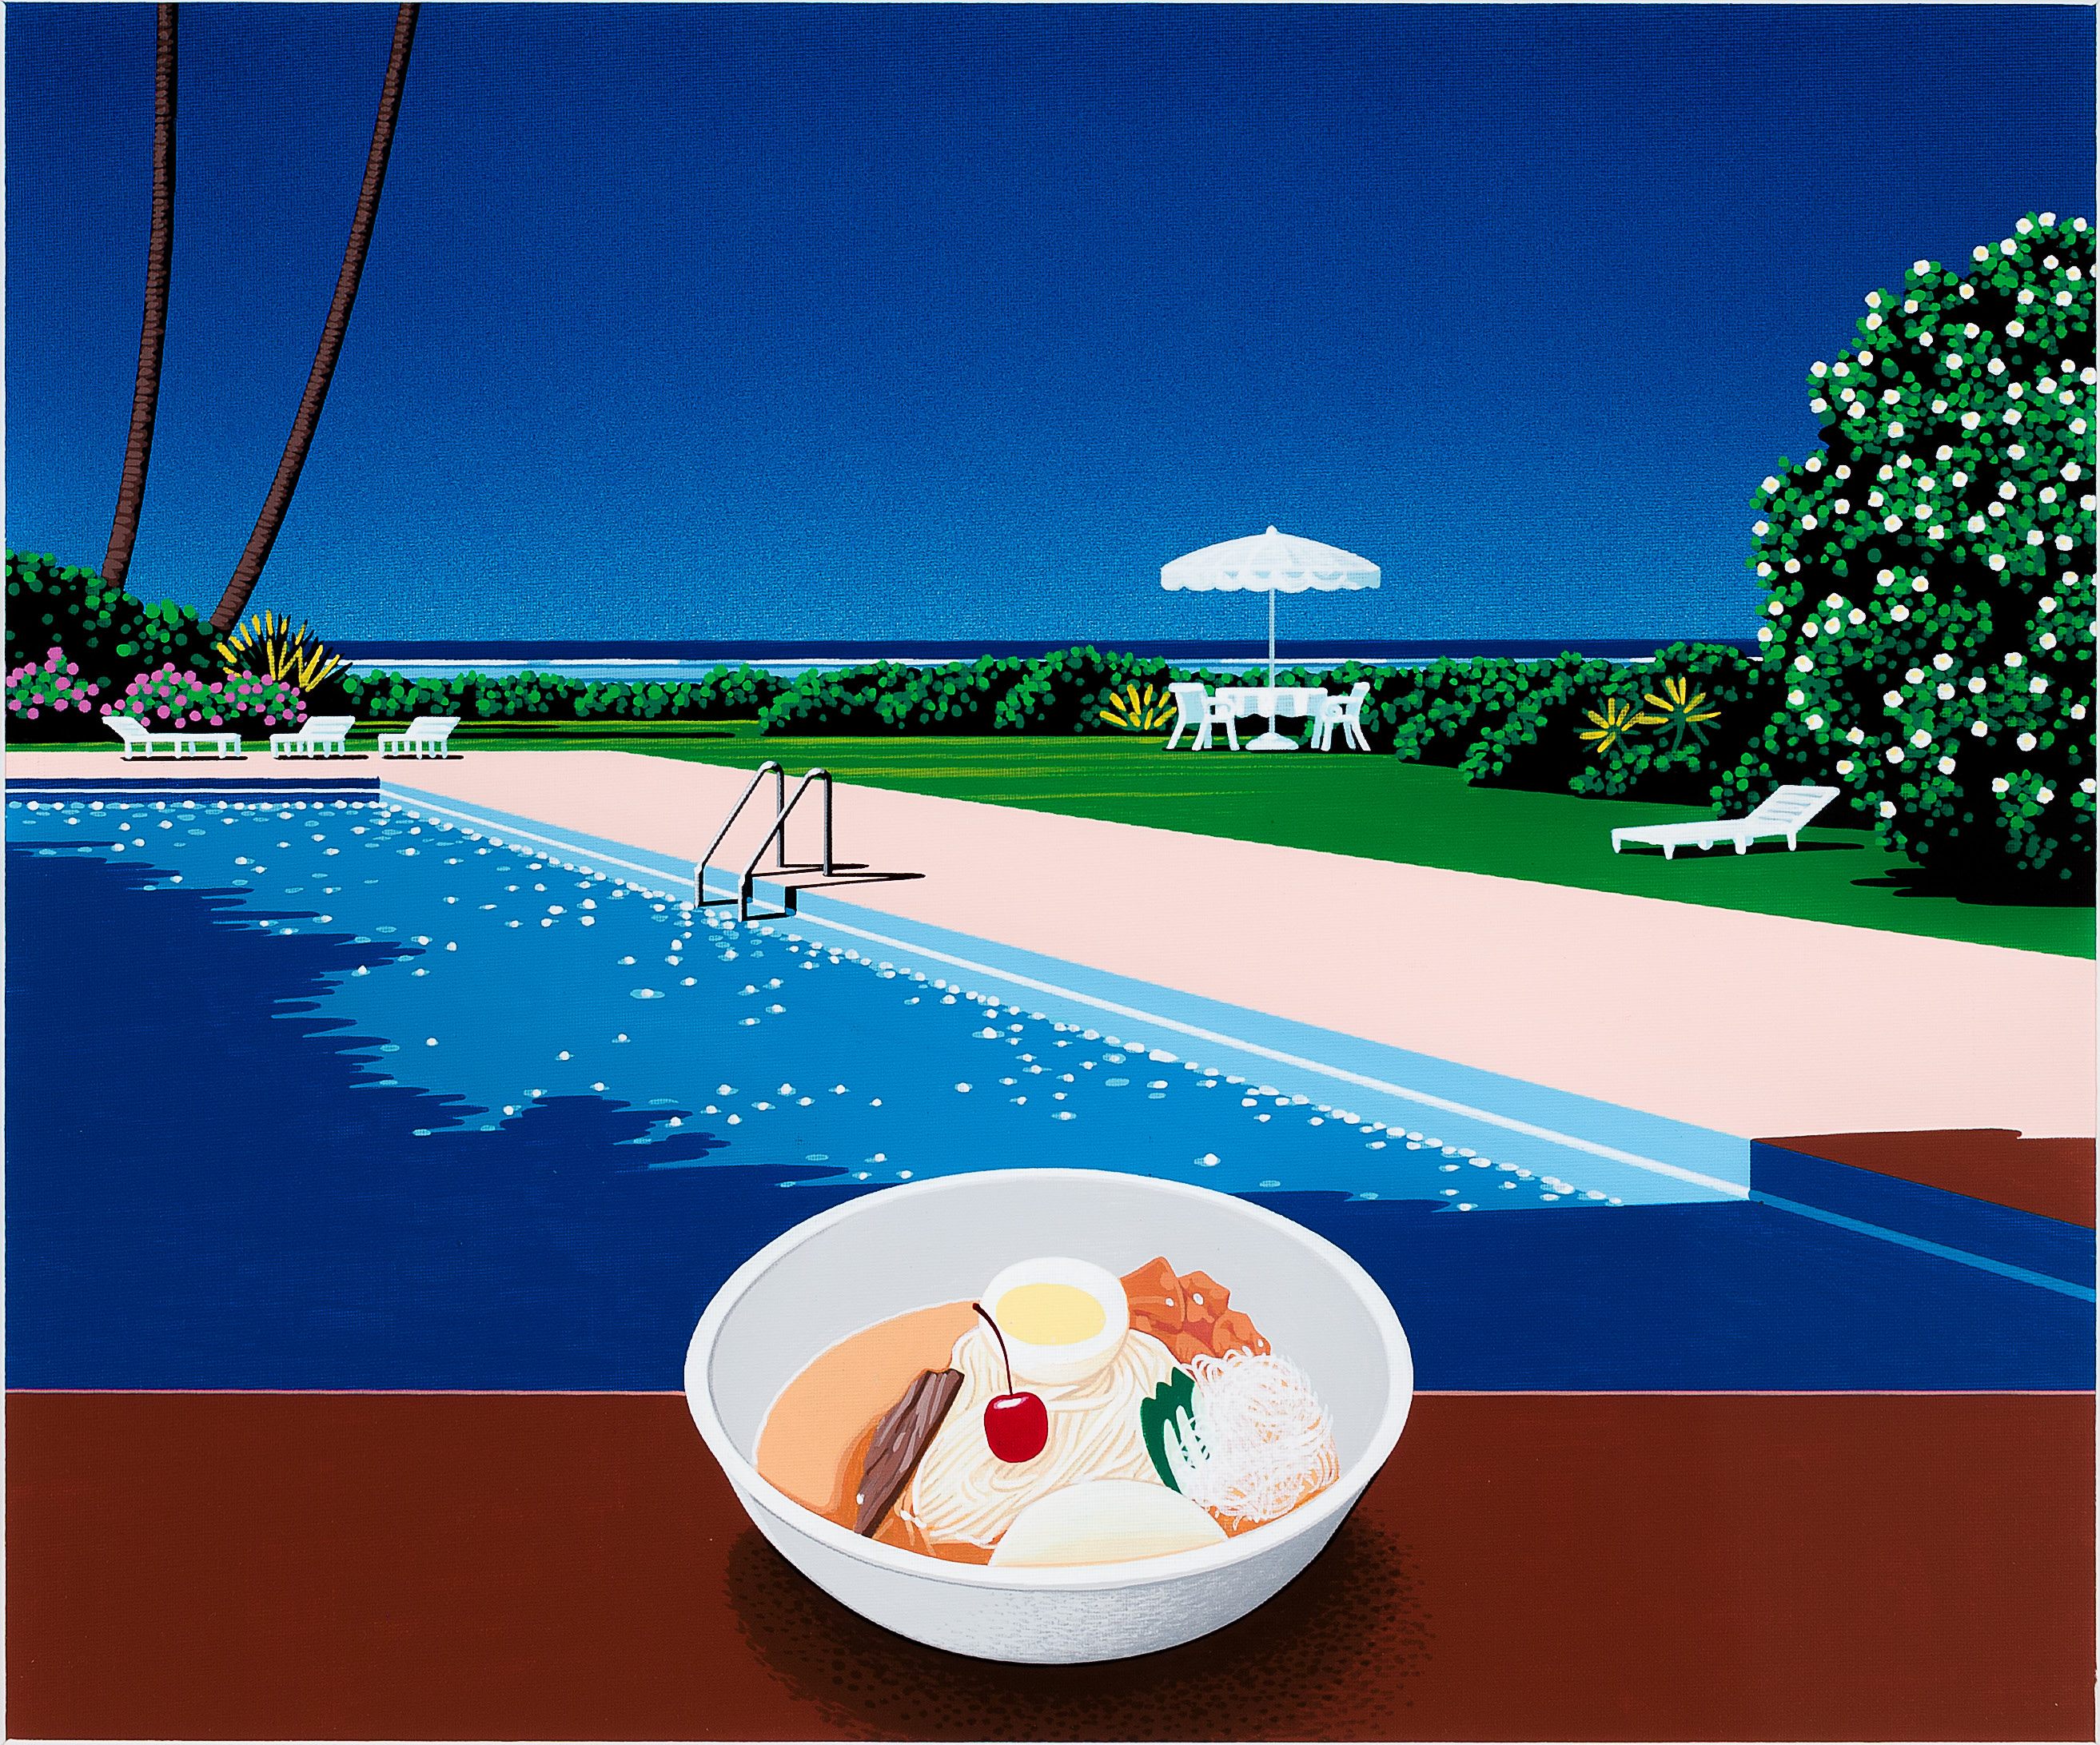
\includegraphics[width=0.52083in,height=\textheight,keepaspectratio]{img/jpf/36.jpg}
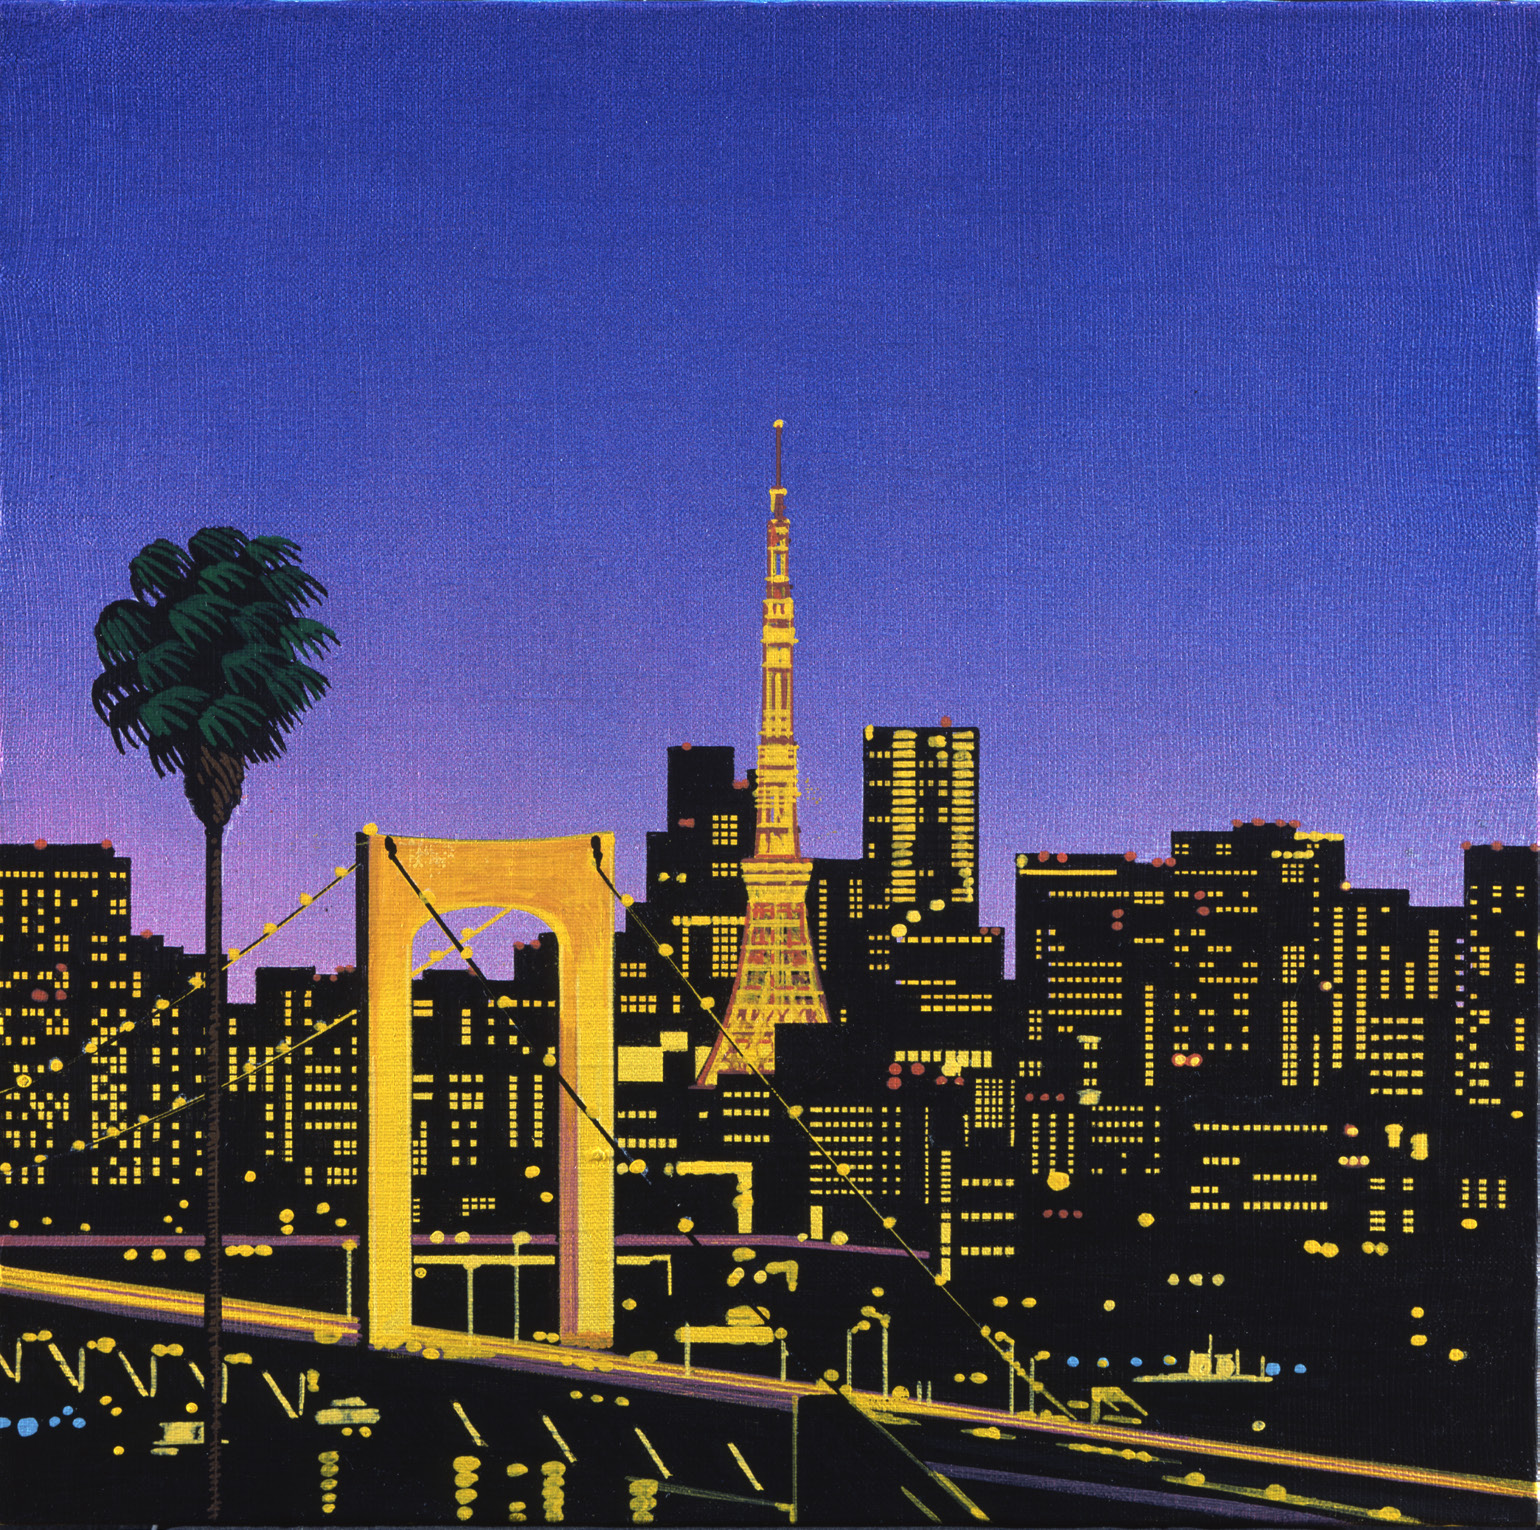
\includegraphics[width=0.52083in,height=\textheight,keepaspectratio]{img/jpf/37.jpg}
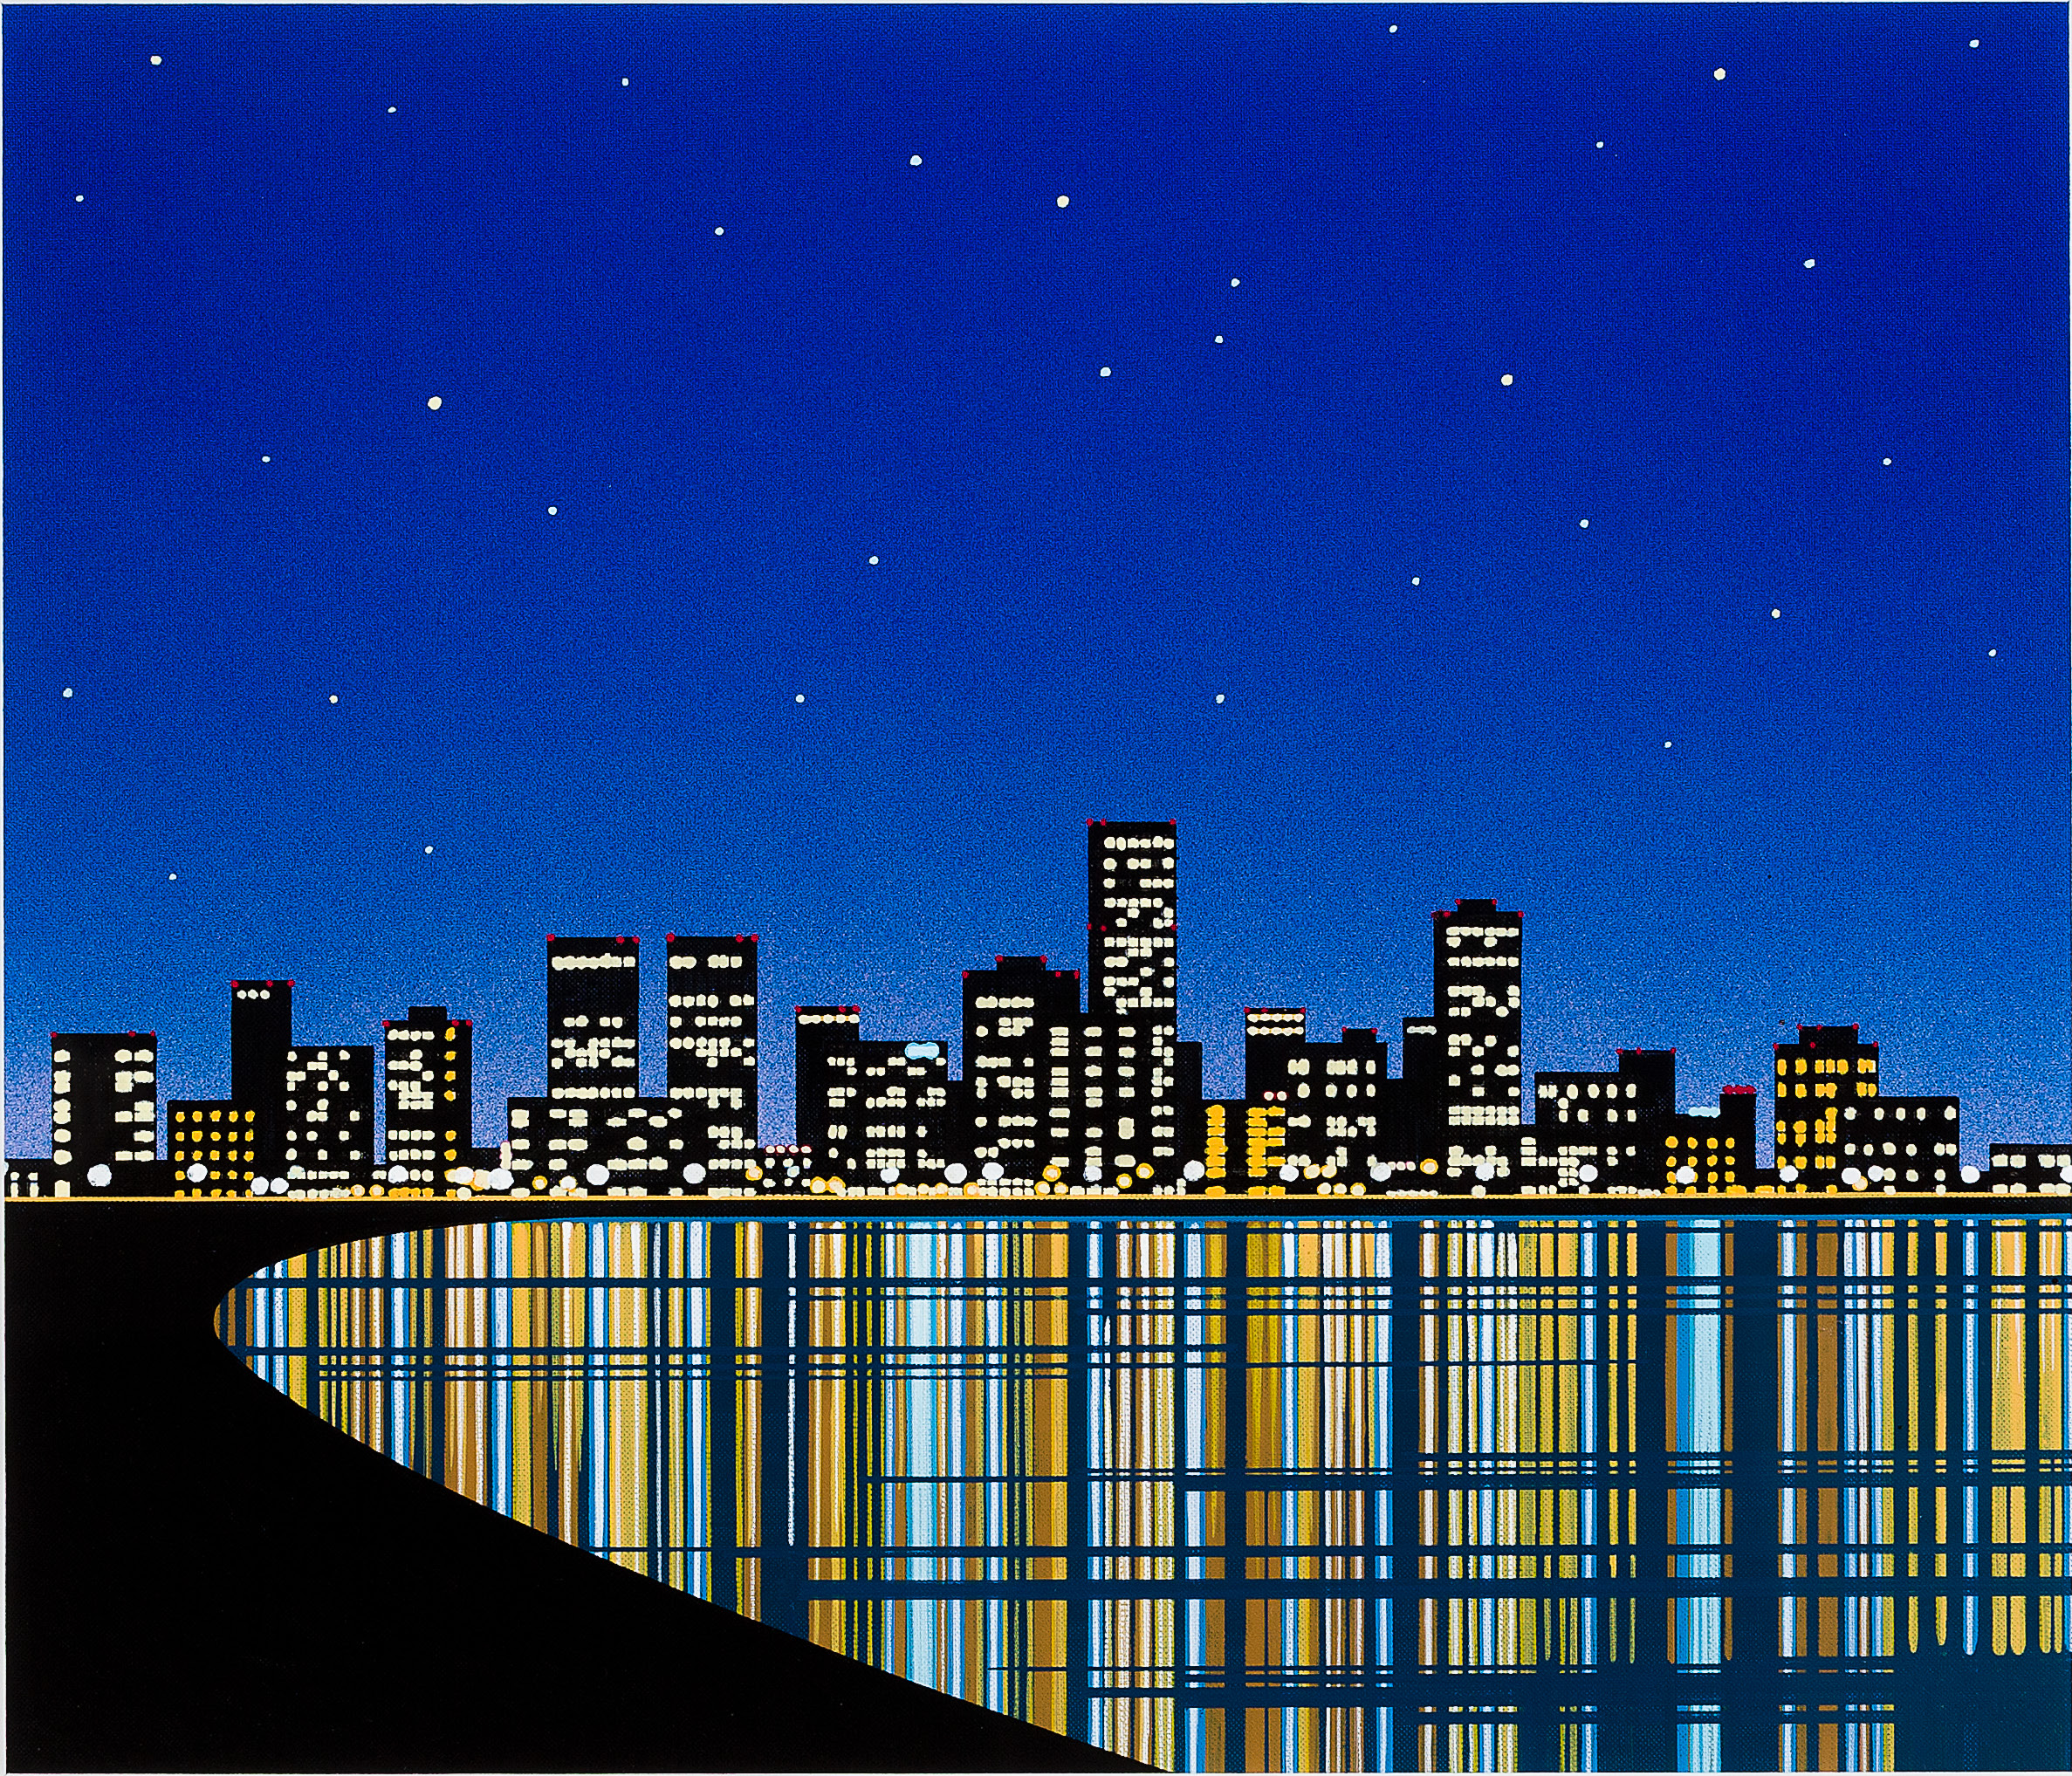
\includegraphics[width=0.52083in,height=\textheight,keepaspectratio]{img/jpf/38.jpg}
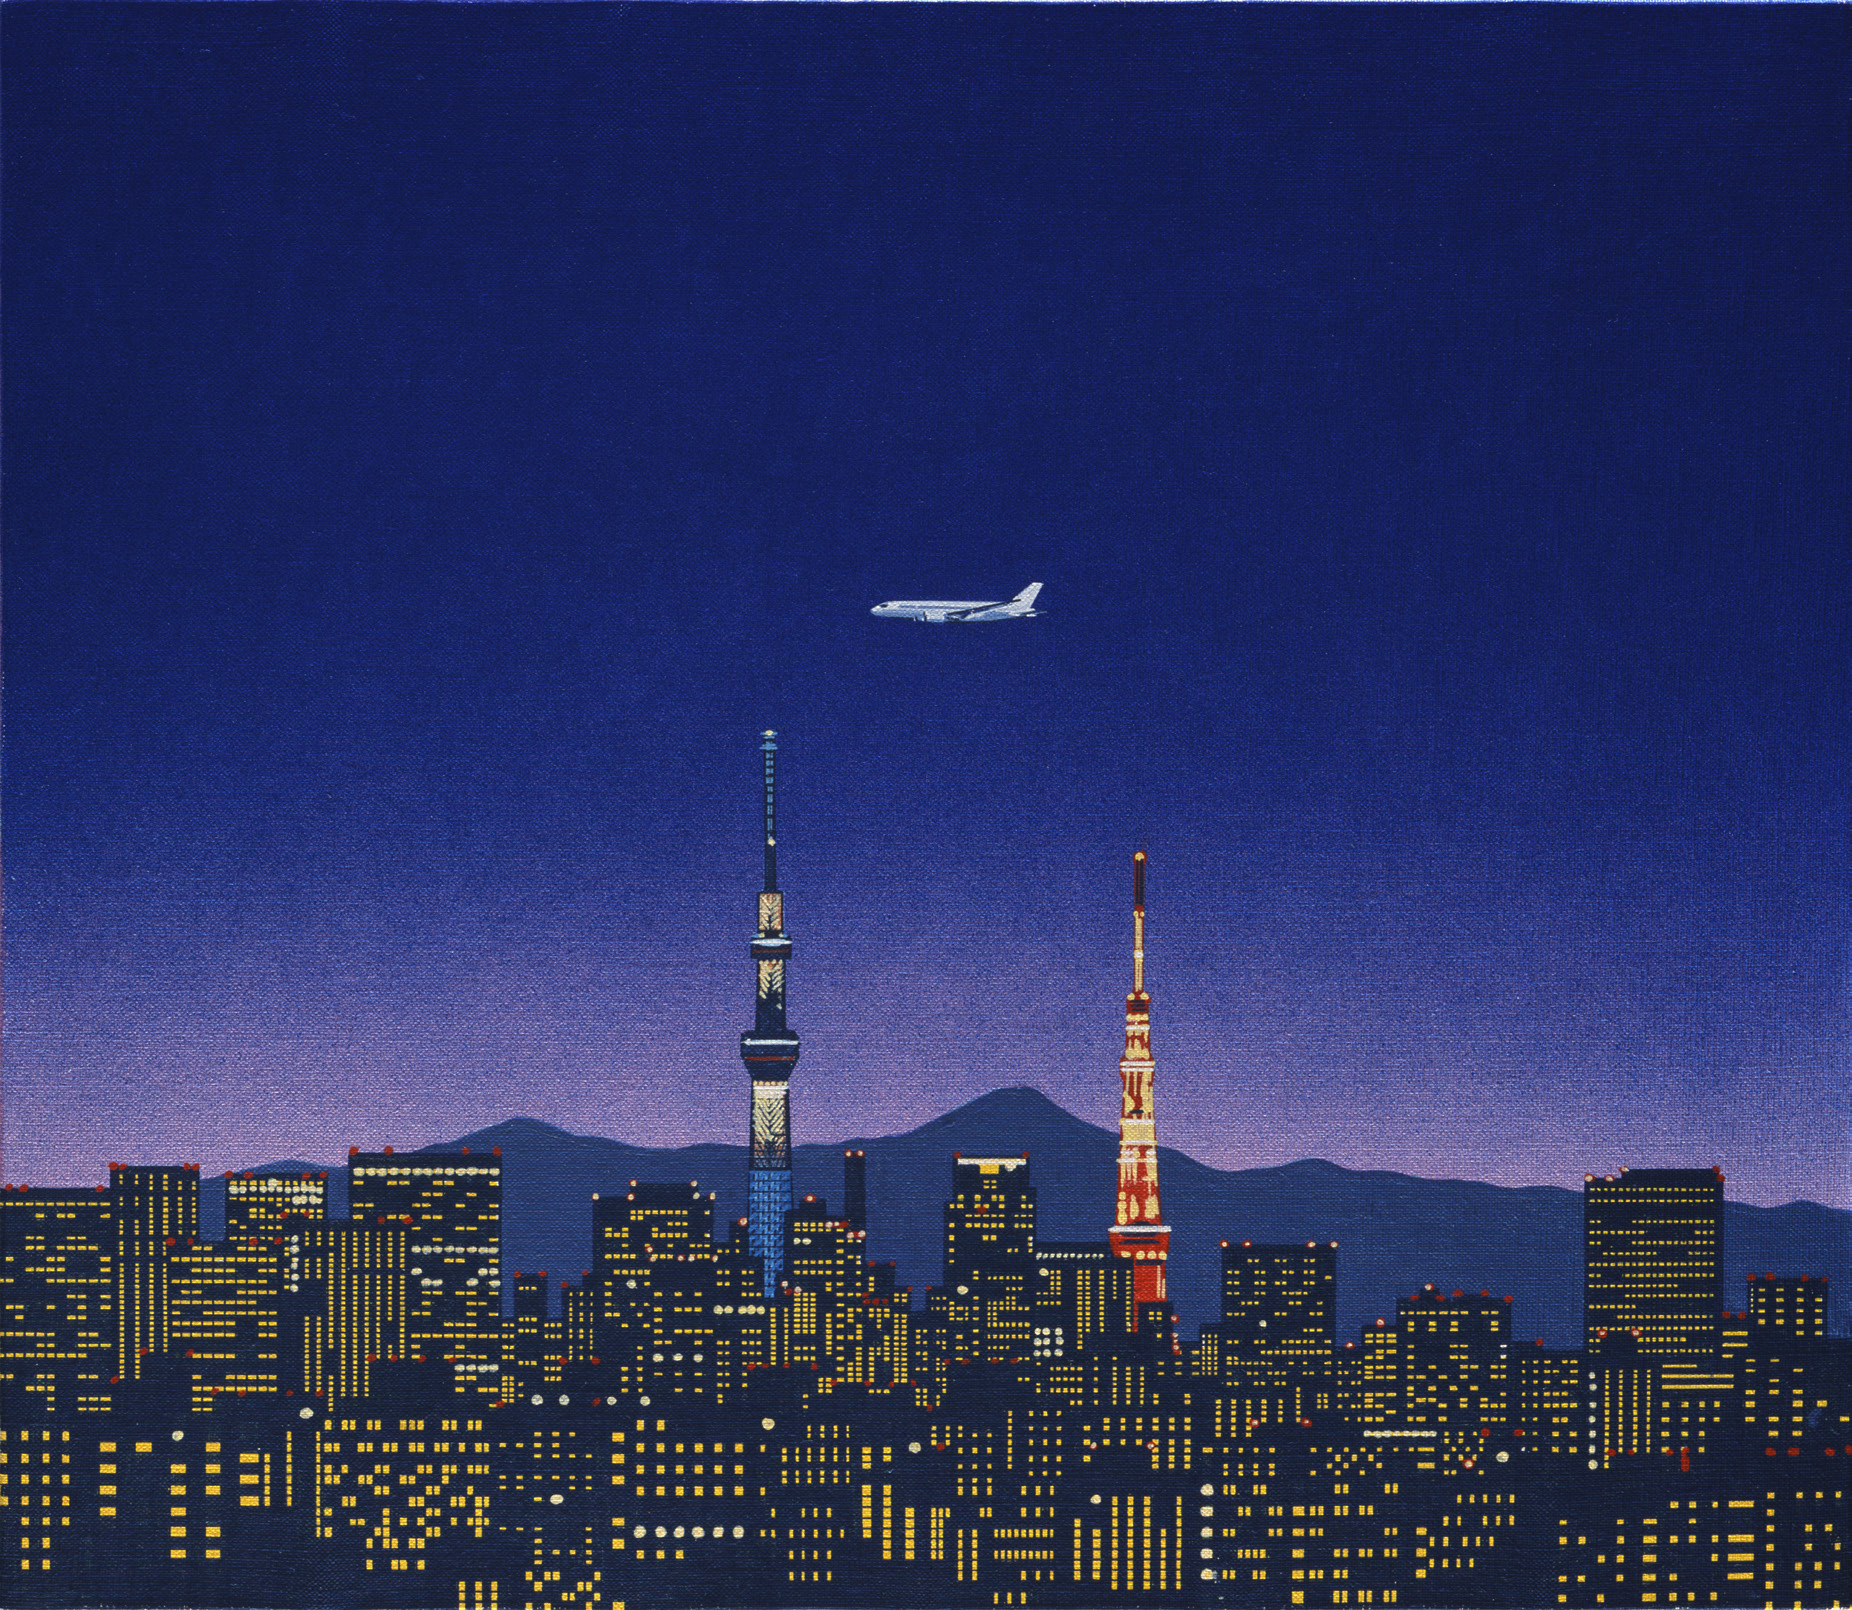
\includegraphics[width=0.52083in,height=\textheight,keepaspectratio]{img/jpf/39.jpg}
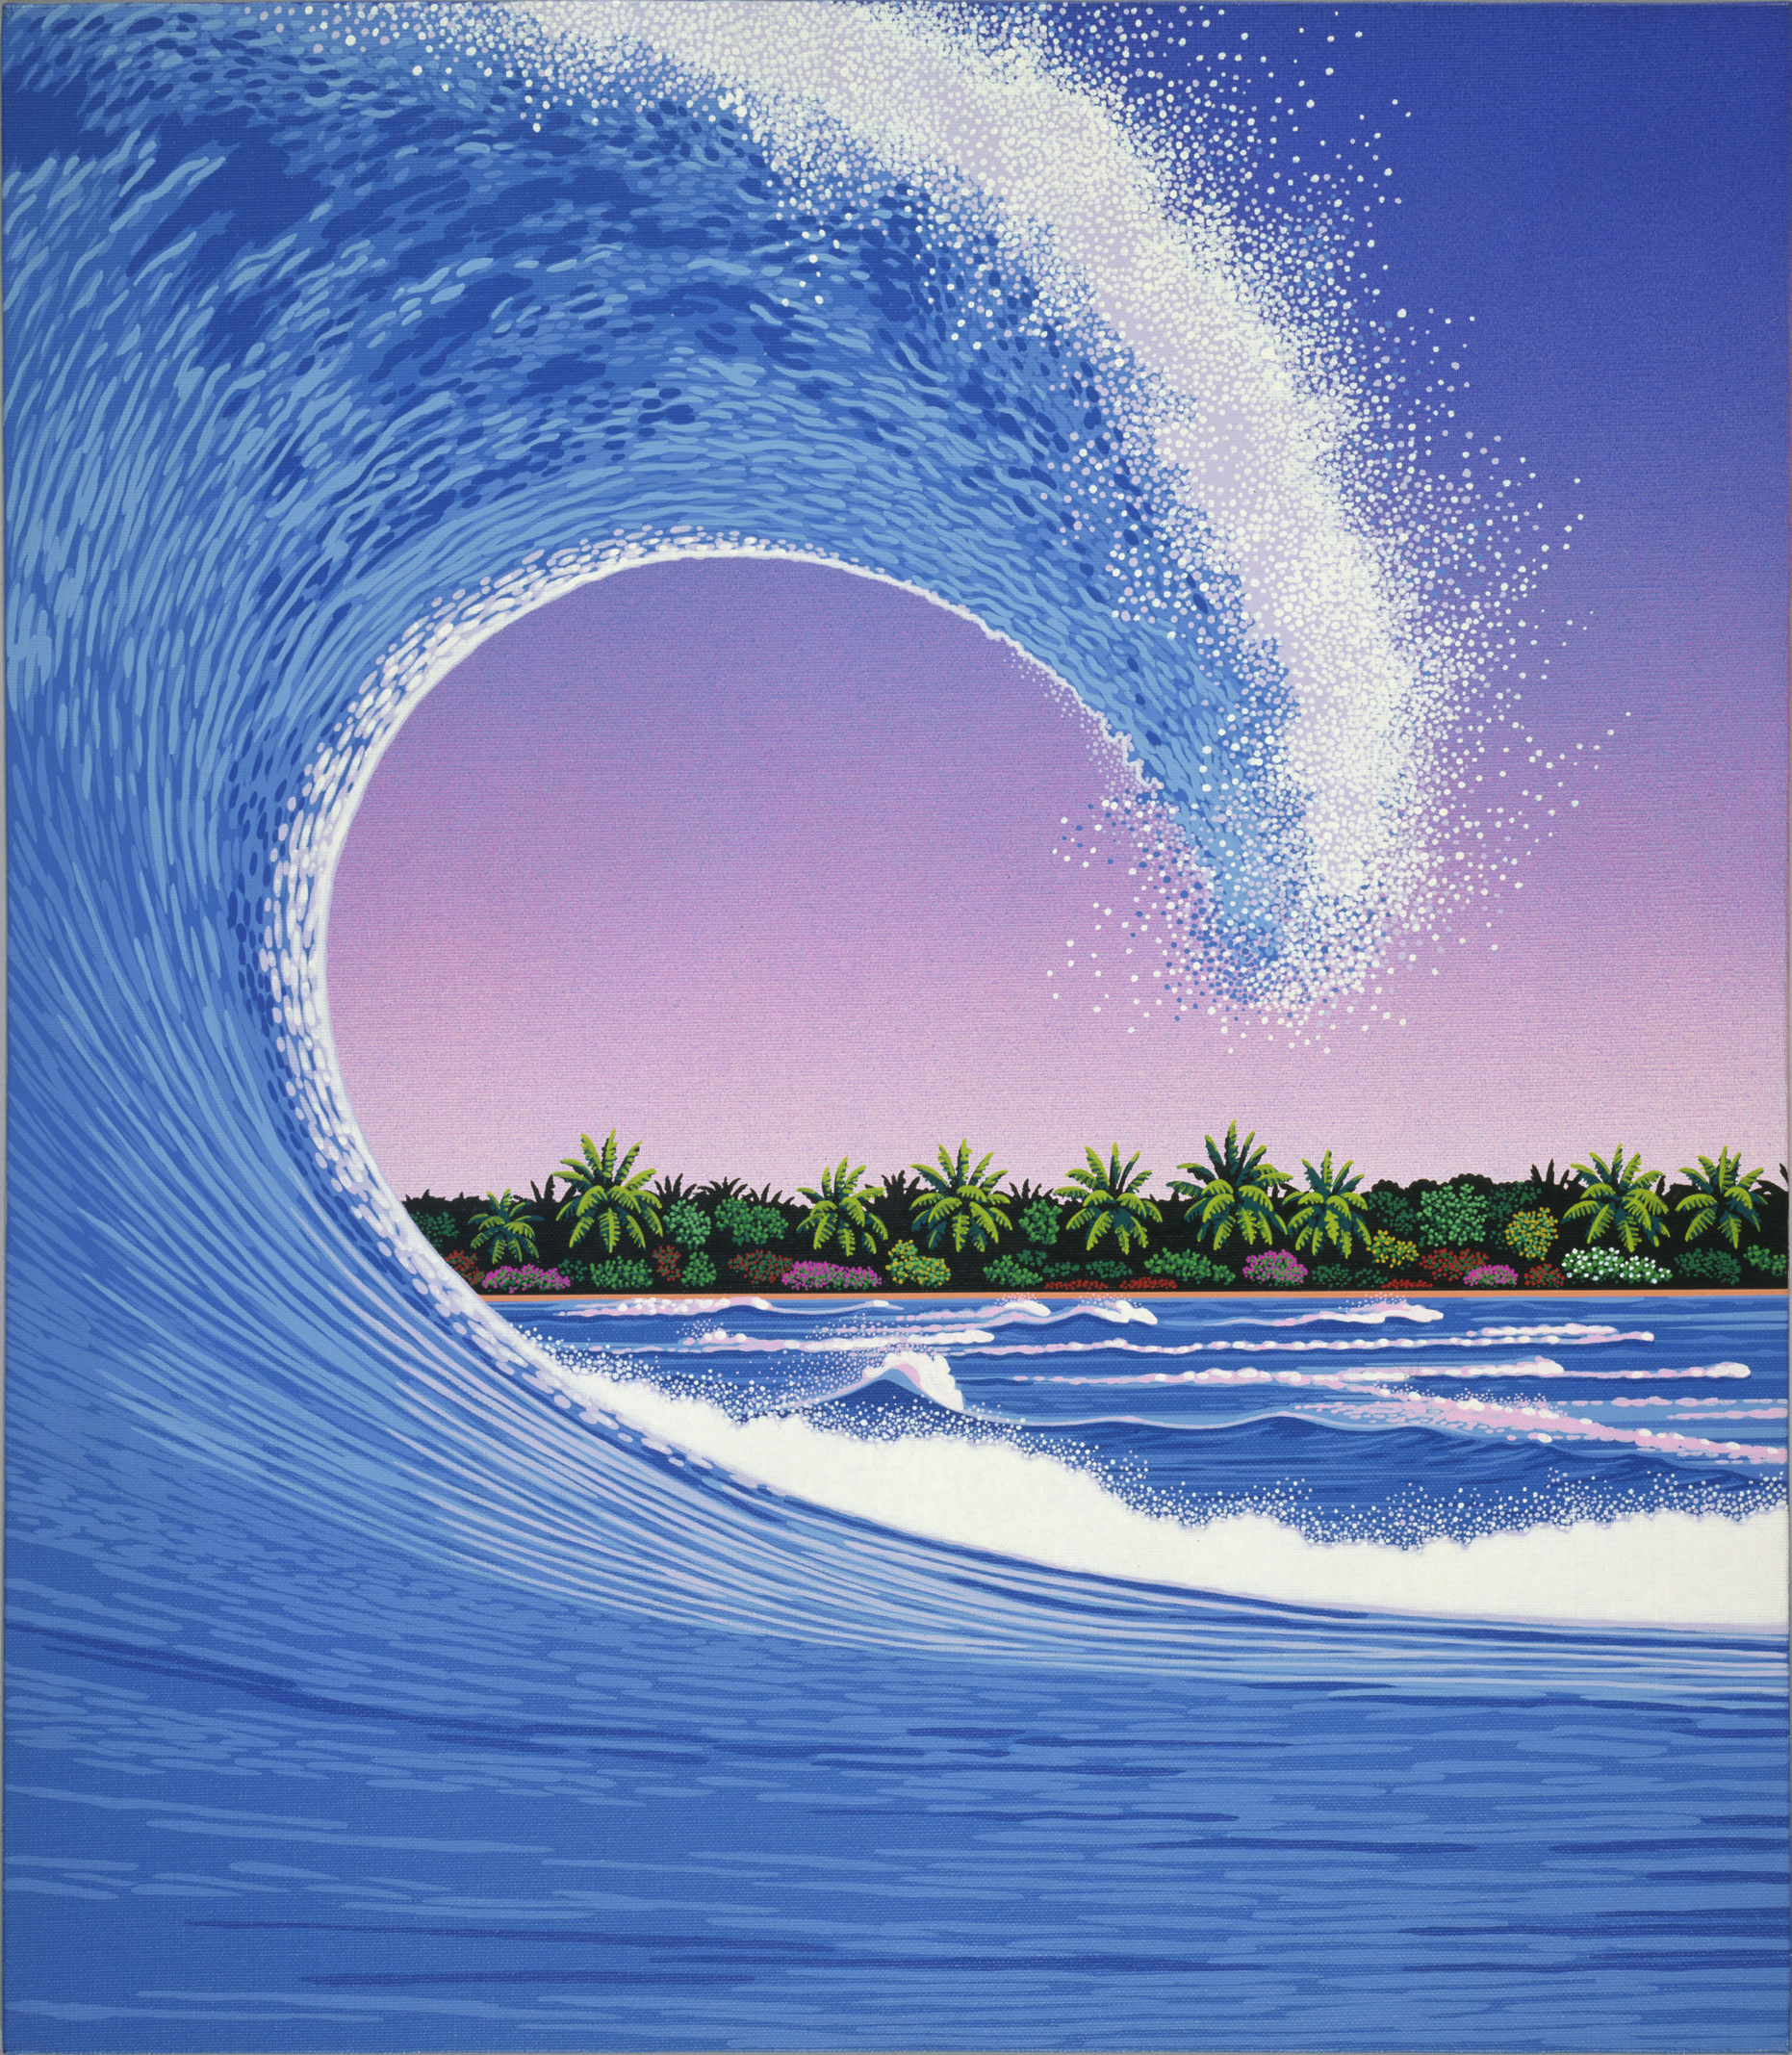
\includegraphics[width=0.52083in,height=\textheight,keepaspectratio]{img/jpf/40.jpg}
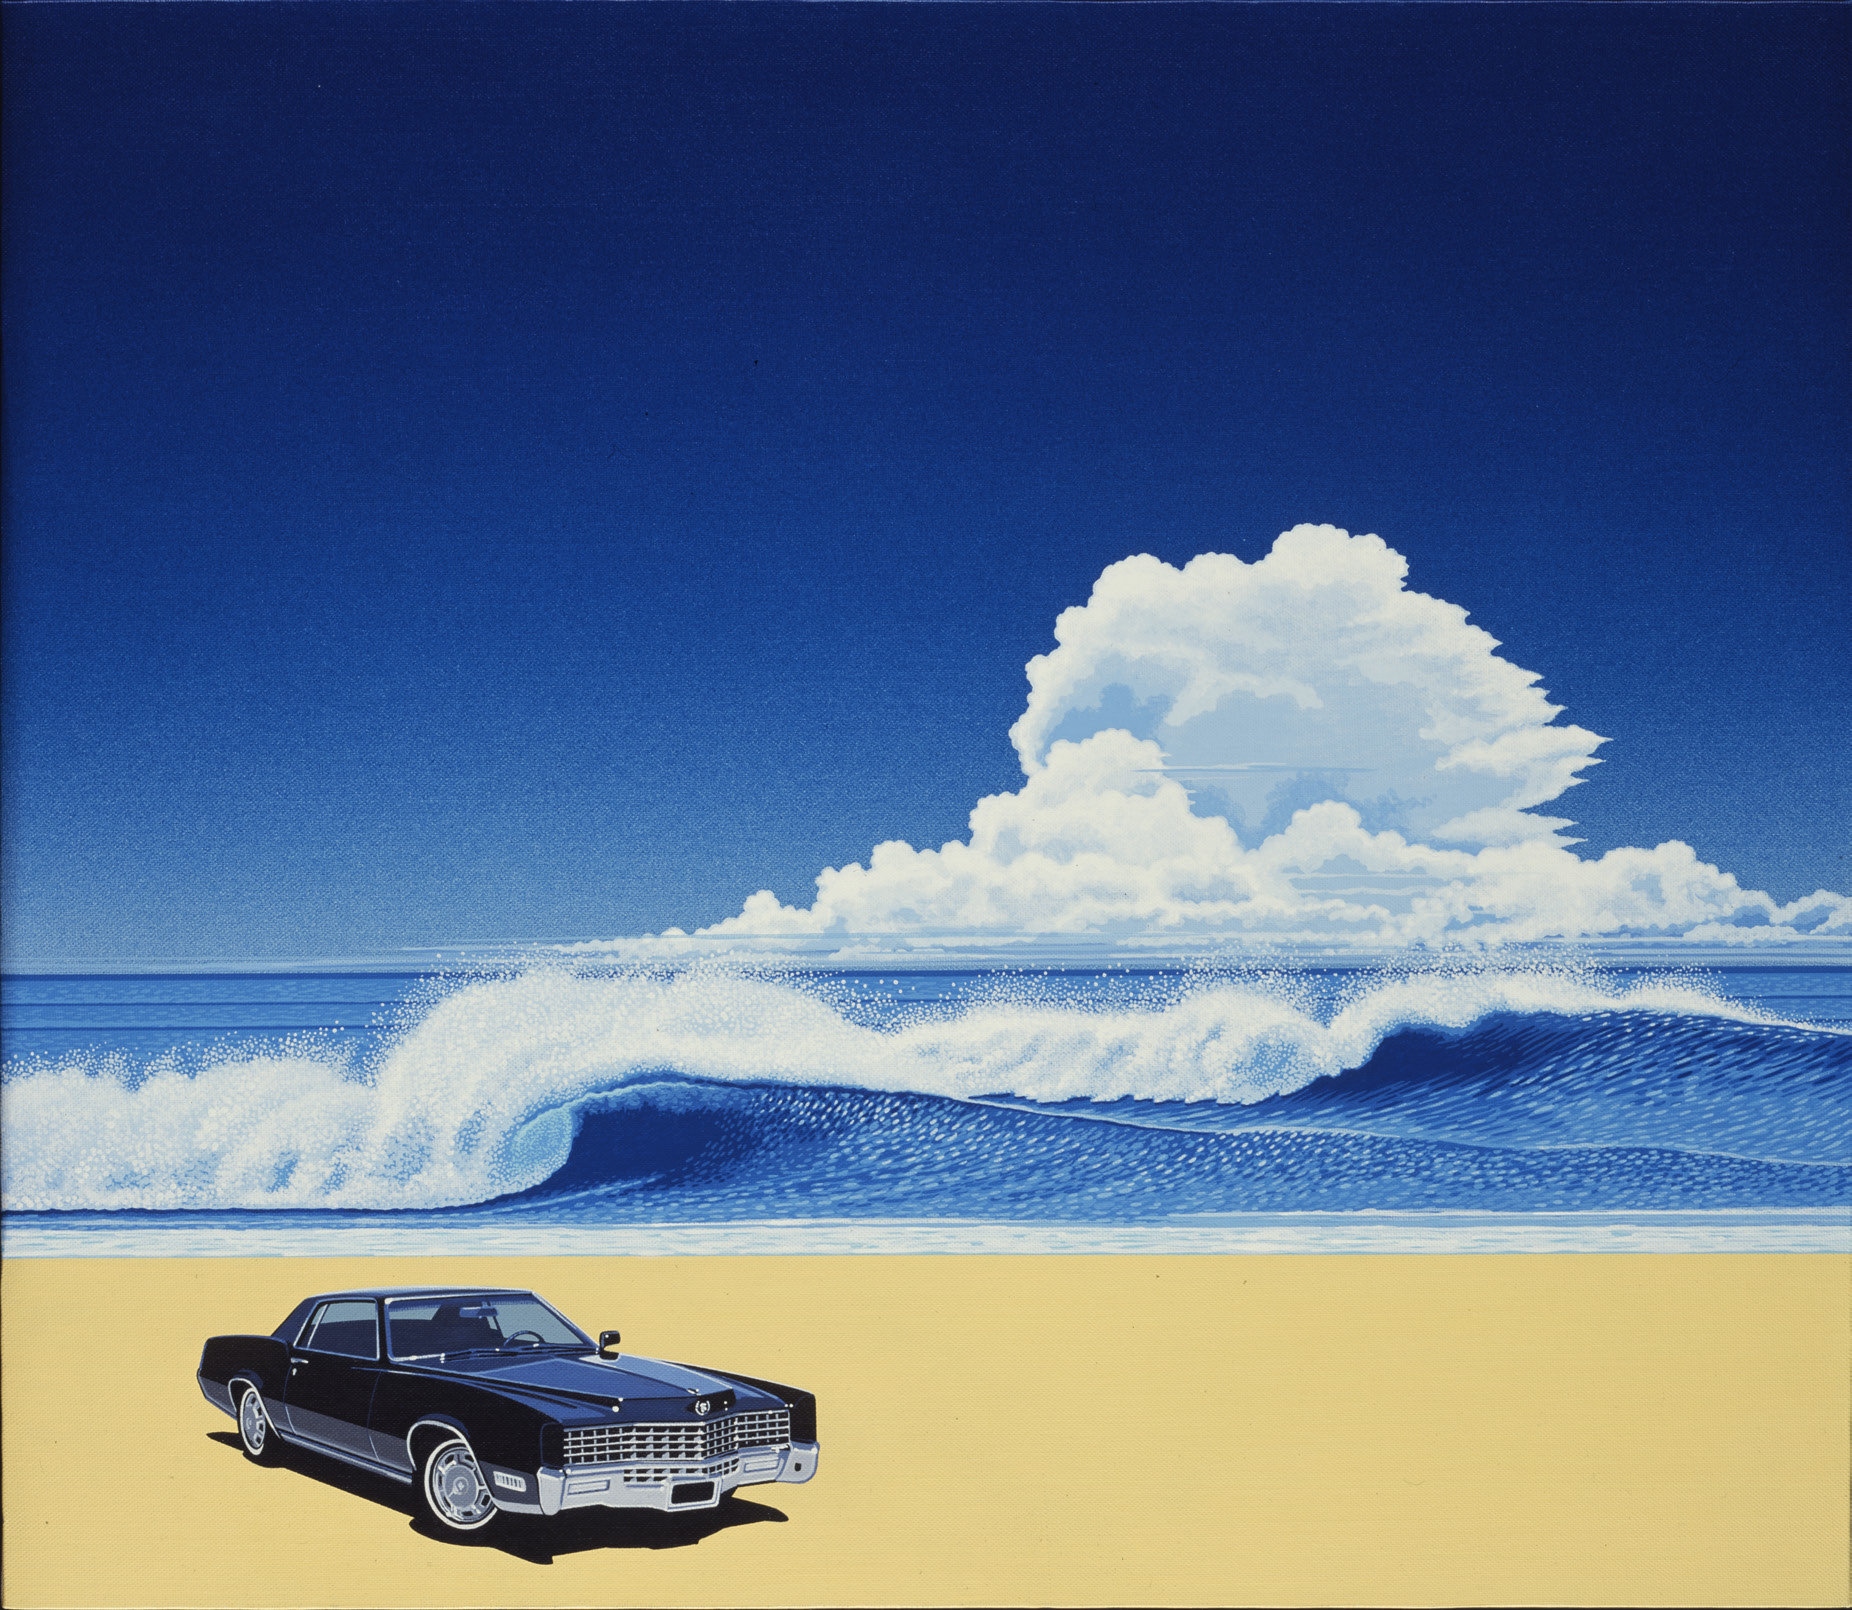
\includegraphics[width=0.52083in,height=\textheight,keepaspectratio]{img/jpf/41.jpg}
\includegraphics[width=0.52083in,height=\textheight,keepaspectratio]{img/jpf/42.jpg}

\end{footnotesize}}

\pandocbounded{\includegraphics[keepaspectratio]{img/plastic-love.webp}}

\begin{center}\rule{0.5\linewidth}{0.5pt}\end{center}

\subsubsection{References}\label{references}

https://www.japantimes.co.jp/culture/2018/11/17/music/mariya-takeuchi-pop-genius-behind-2018s-surprise-online-smash-hit-japan/




\end{document}
